%
% The first command in your LaTeX source must be the \documentclass command.
\documentclass[sigchi]{acmart}
\usepackage{graphicx}
%
% defining the \BibTeX command - from Oren Patashnik's original BibTeX documentation.
\def\BibTeX{{\rm B\kern-.05em{\sc i\kern-.025em b}\kern-.08emT\kern-.1667em\lower.7ex\hbox{E}\kern-.125emX}}
    
% Rights management information. 
% This information is sent to you when you complete the rights form.
% These commands have SAMPLE values in them; it is your responsibility as an author to replace
% the commands and values with those provided to you when you complete the rights form.
%
% These commands are for a PROCEEDINGS abstract or paper.
\copyrightyear{2019}
\acmYear{2019}
\setcopyright{acmlicensed}
\acmConference[SNA '22]{Social Network Analysis '22}{2021/22}{University of Pisa, Italy}
\acmBooktitle{Social Network Analysis '22}
\acmPrice{0.00}
%\acmDOI{10.1145/1122445.1122456}
%\acmISBN{978-1-4503-9999-9/18/06}


% end of the preamble, start of the body of the document source.
\begin{document}

%
% The "title" command has an optional parameter, allowing the author to define a "short title" to be used in page headers.
\title{Networks of shares: SP500 from 1962 to 2022}

%
% The "author" command and its associated commands are used to define the authors and their affiliations.
% Of note is the shared affiliation of the first two authors, and the "authornote" and "authornotemark" commands
% used to denote shared contribution to the research.
\author{Manuel Luci}
\email{m.luci@studenti.unipi.it}
\affiliation{%
  \institution{Student ID: 581770}
}

\author{Ayushy Vijaykuma }
\email{a.vijaykumar@studenti.unipi.it}
\affiliation{%
  \institution{Student ID:626233}
}

\author{Alessandro Seccarelli}
\email{a.seccarellli@studenti.unipi.it}
\affiliation{%
  \institution{Student ID: 583814}
}




\renewcommand{\shortauthors}{One and Two, et al.}


% The abstract is a short summary of the work to be presented in the article.
\begin{abstract}
In this project, we aim to study the stock market with the tools of graph theory. 
In particular, we will study the static and dynamic properties of the graph obtained by considering as nodes the individual stocks included in the SP500 index, and as adjacency relation being strongly correlated. 
After a quick statistical study of the general topological characteristics of the graph obtained by considering the entire temporal span (1962-2022), we will devote attention to community discovery, both in the dynamic and static case, attempting to make identifications with the ground truth offered to us by the sectoral affiliation of the various firms. 
The results on this issue tend to be negative, as it is not possible to draw conclusions that support the initial hypothesis of coincidence between communities and sectoral grouping.
Finally, we will investigate whether and how the major events disrupting the world's stock exchanges can be traced in our data: above all, the two most recent financial crushes ( subprime mortgage crisis and the global pandemic).

\footnote{
{\bf Project Repositories}\\
\noindent Data Collection: \url{https://github.com/sna-unipi/sna-project-2022_luci_seccarelli_ayushi/tree/main/data_collection}\\
\noindent Analytical Tasks: \url{https://github.com/sna-unipi/analytical-tasks}\\
\noindent Report: \url{https://github.com/sna-unipi/sna-project-2022_luci_seccarelli_ayushi/tree/main/report}}
\end{abstract}


%
% Keywords. The author(s) should pick words that accurately describe the work being
% presented. Separate the keywords with commas.
\keywords{Social Network Analysis, Stock market network, Financial crushes, Speculative bubble, Communities}

%
% This command processes the author and affiliation and title information and builds
% the first part of the formatted document.
\maketitle

\section{Introduction}
Social Network analysis is a useful tool to analyse the stock market: the graph has firm as nodes and "strength" of correlation as edge. In the following project we have considered only strong correlation (Pearson correlation $> 0.8$) and negative one (Pearson correlation $< -0.5$).
\section{Data Collection}
As source we have considered Yahoo Finance and through the package \textsc{yfinance} we get annual historic data for each firm of S\&P 500 since 1962, we saved it in a dictionary where each key is a stock (\textbf{dataset\_building.py}). We build a  yearly correlation matrix (evaluate pearson correlation of adjusted closed price) and saved them in a dictionary, each key is the considered year, we cleaned them (deleting NaN values and 0 values),
(\textbf{correlation\_building, cleaning\_correlation, correlation\_building\_aggregate)}.\\
As last step we built graph using this data (node: stocks, edge: correlation, label : sector): \texttt{list\_pos\_graph\_label.npy} is a dictionary of strongly correlated stocks,\\ \texttt{list\_neg\_graph\_label.npy} is a dictionary of inversely correlated stocks, each key is a year; \texttt{pos\_graph\_tot.gpickle} and \texttt{neg\_graph\_tot.gpickle} are graph strongly and negatively correlated obtained considering the entire timeline (\textbf{graph\_building, graph\_splitting, label\_graph)}. 
\section{Network Analysis}
\subsection{Static Network}
First of all we analyzed statistical behaviour of static network (we call positive = strongly correlated network, negative = weakly correlated network); both positive and negative have 494 nodes, but positive has 70567 edges, negative 1026, the average degree of positive is 285.70 while negative is 4.15. \\ Studying the distribution of degree gives useful information about graph's topology: plotting both distribution in loglog scale shows a power law behaviour for the negative one:
\begin{figure}[h]
	\centering
	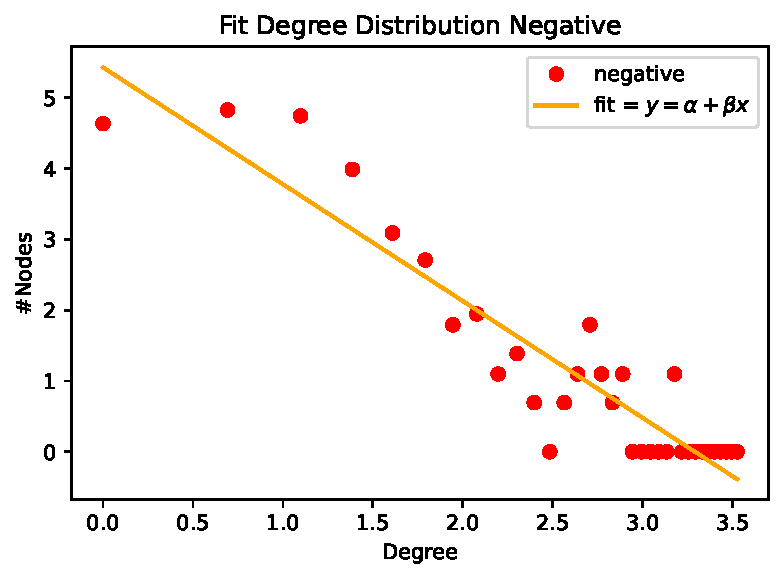
\includegraphics[width=\linewidth]{plot/degree_distribution_negative_fit.pdf}
	\caption{Degree Distribution negative graph fit}
\end{figure}
\begin{figure}[h]
	\centering
	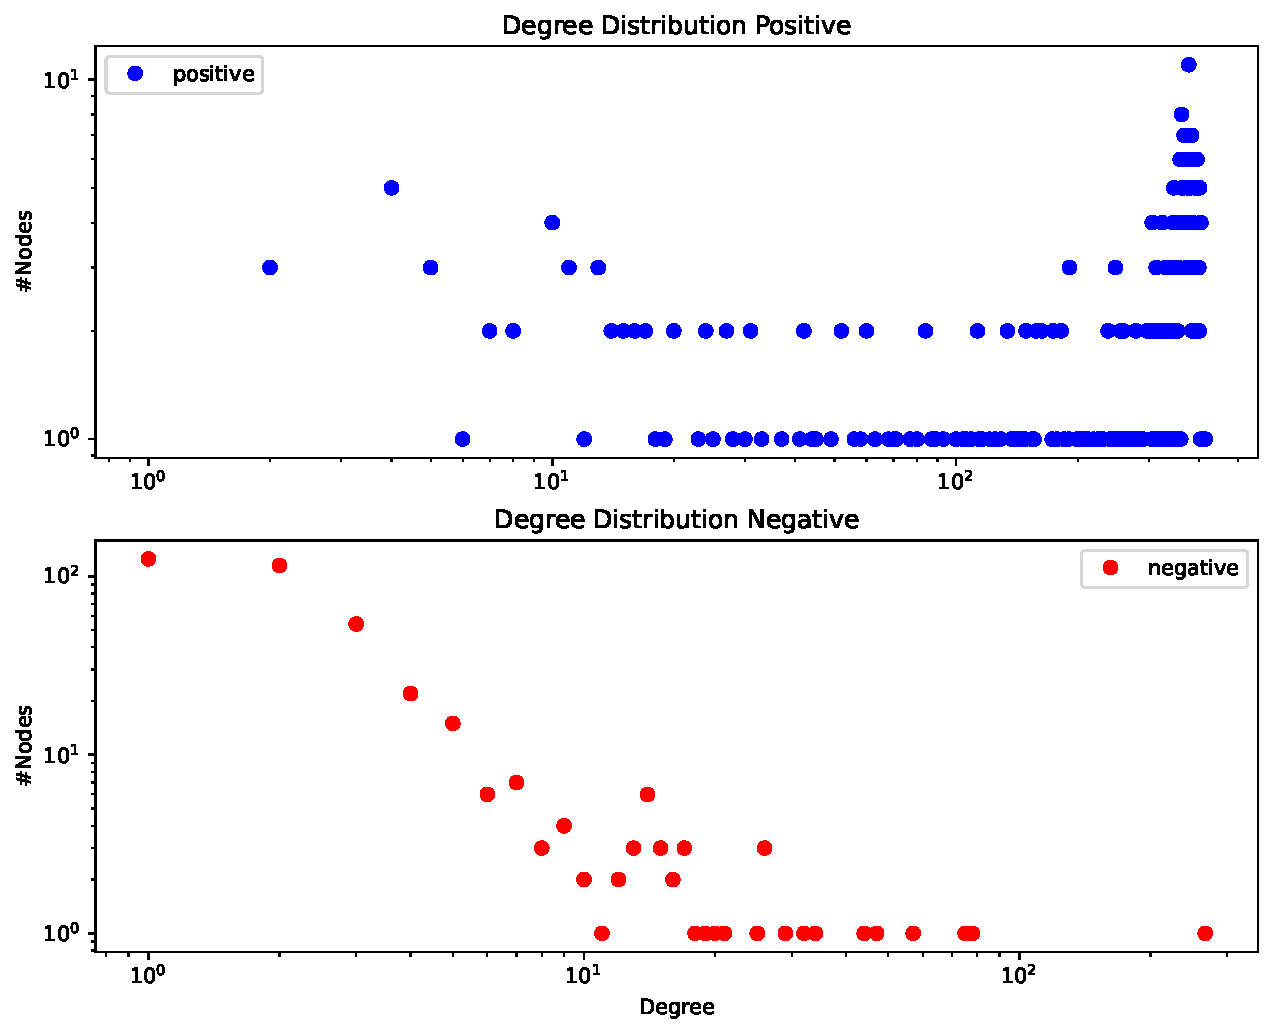
\includegraphics[width=\linewidth]{plot/degree_distribution.pdf}
	\caption{Degree Distribution positive and negative graph}
\end{figure}
Fitting a powerlaw distribution $y= \alpha + \beta x$ ($y$ = number of nodes, $x = \log$(degree)), we obtain: $\alpha = 5.43 \pm 0.30, \beta = -1.65 \pm 0.11, R2 = 0.87, \chi^2 = 0.99$, this result is in agreement with general financial theory.\\
Diameter of biggest component of positive is 5, for negative 6 and avarage shortest path are respectively 1.47 and 2.74.\\
Plotting average shortest path distribution for positive, shows powerlaw behaviour, fitting this distribution with $y = Cx^{-\alpha}$ we obtained: $C = 6.01 \pm 0.55, \alpha = 2.71 \pm 0.29, R2 = 0.36, \chi^2 = 172.81$
\begin{figure}[h]
	\centering
	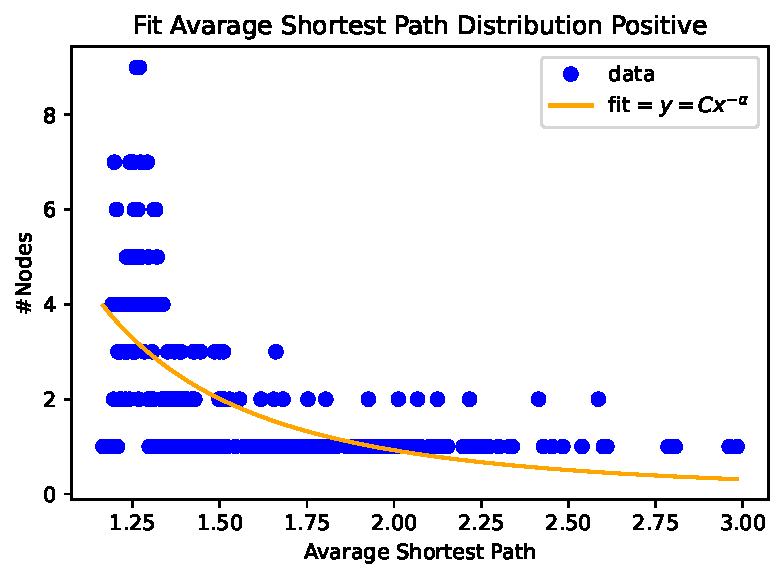
\includegraphics[width=\linewidth]{plot/avarage_shortest_path_distribution_positive_fit.pdf}
	\caption{Average Shortest Path Distribution for Positive }
\end{figure}
Density of positive and negative is 0.58 and 0.01, while global clustering coefficient is 0.834 and 0.001. 
\subsubsection{Comparision with ER}
A ER graph having same edges and nodes of our positive and negative graph need $p = 0.58$ for positive and 0.01 for negative, positive is in  connected regime, negative in supercritical; plotting positive and negative degree distribution we can notice as ER graph is not a good model for our graphs.
\begin{figure}[h]
	\centering
	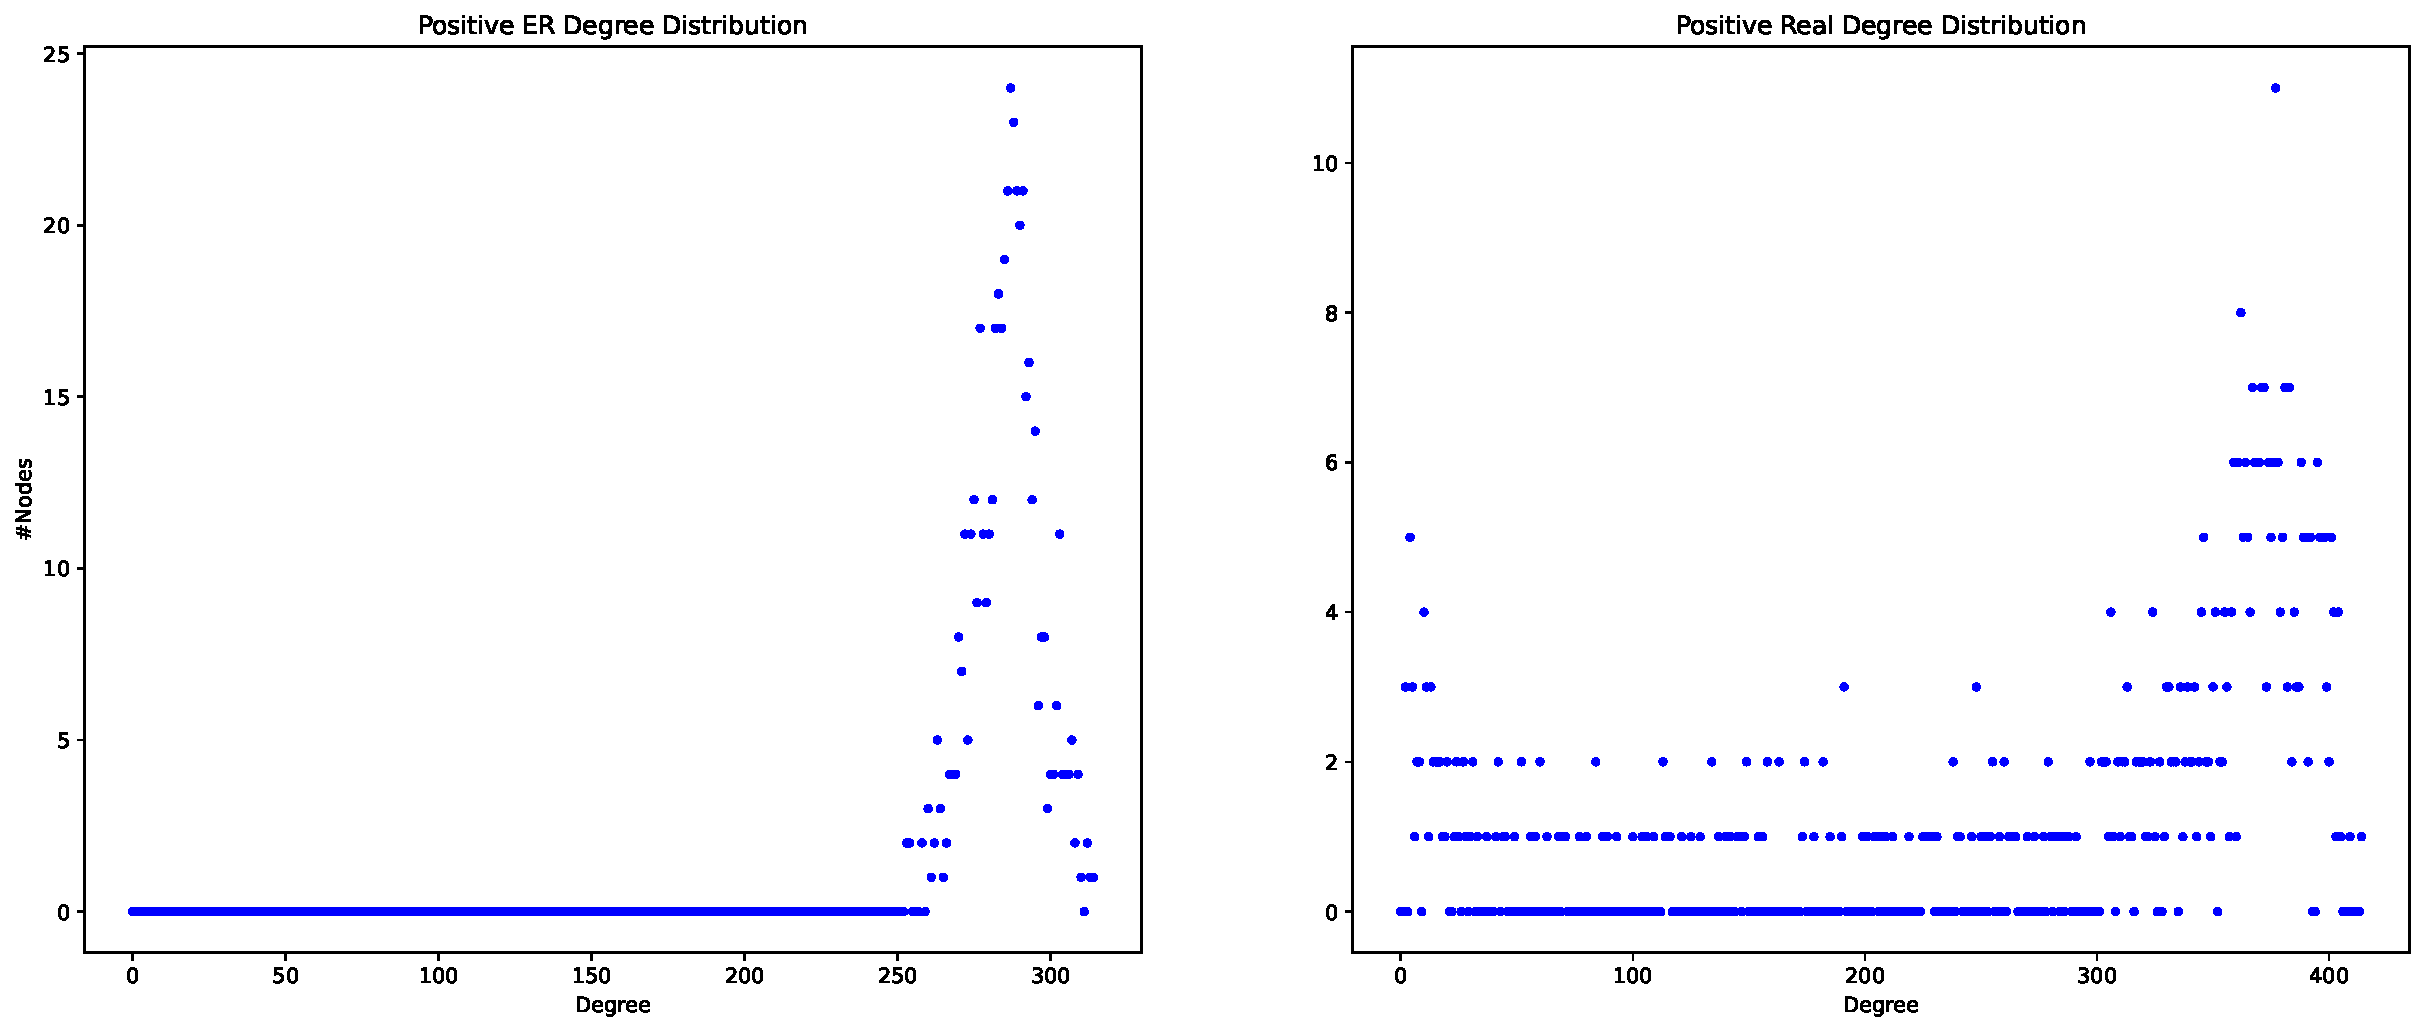
\includegraphics[width=\linewidth]{plot/er_comparison_positive.pdf}
	\caption{Positive ER Degree Distribution}
\end{figure}
\begin{figure}[h]
	\centering
	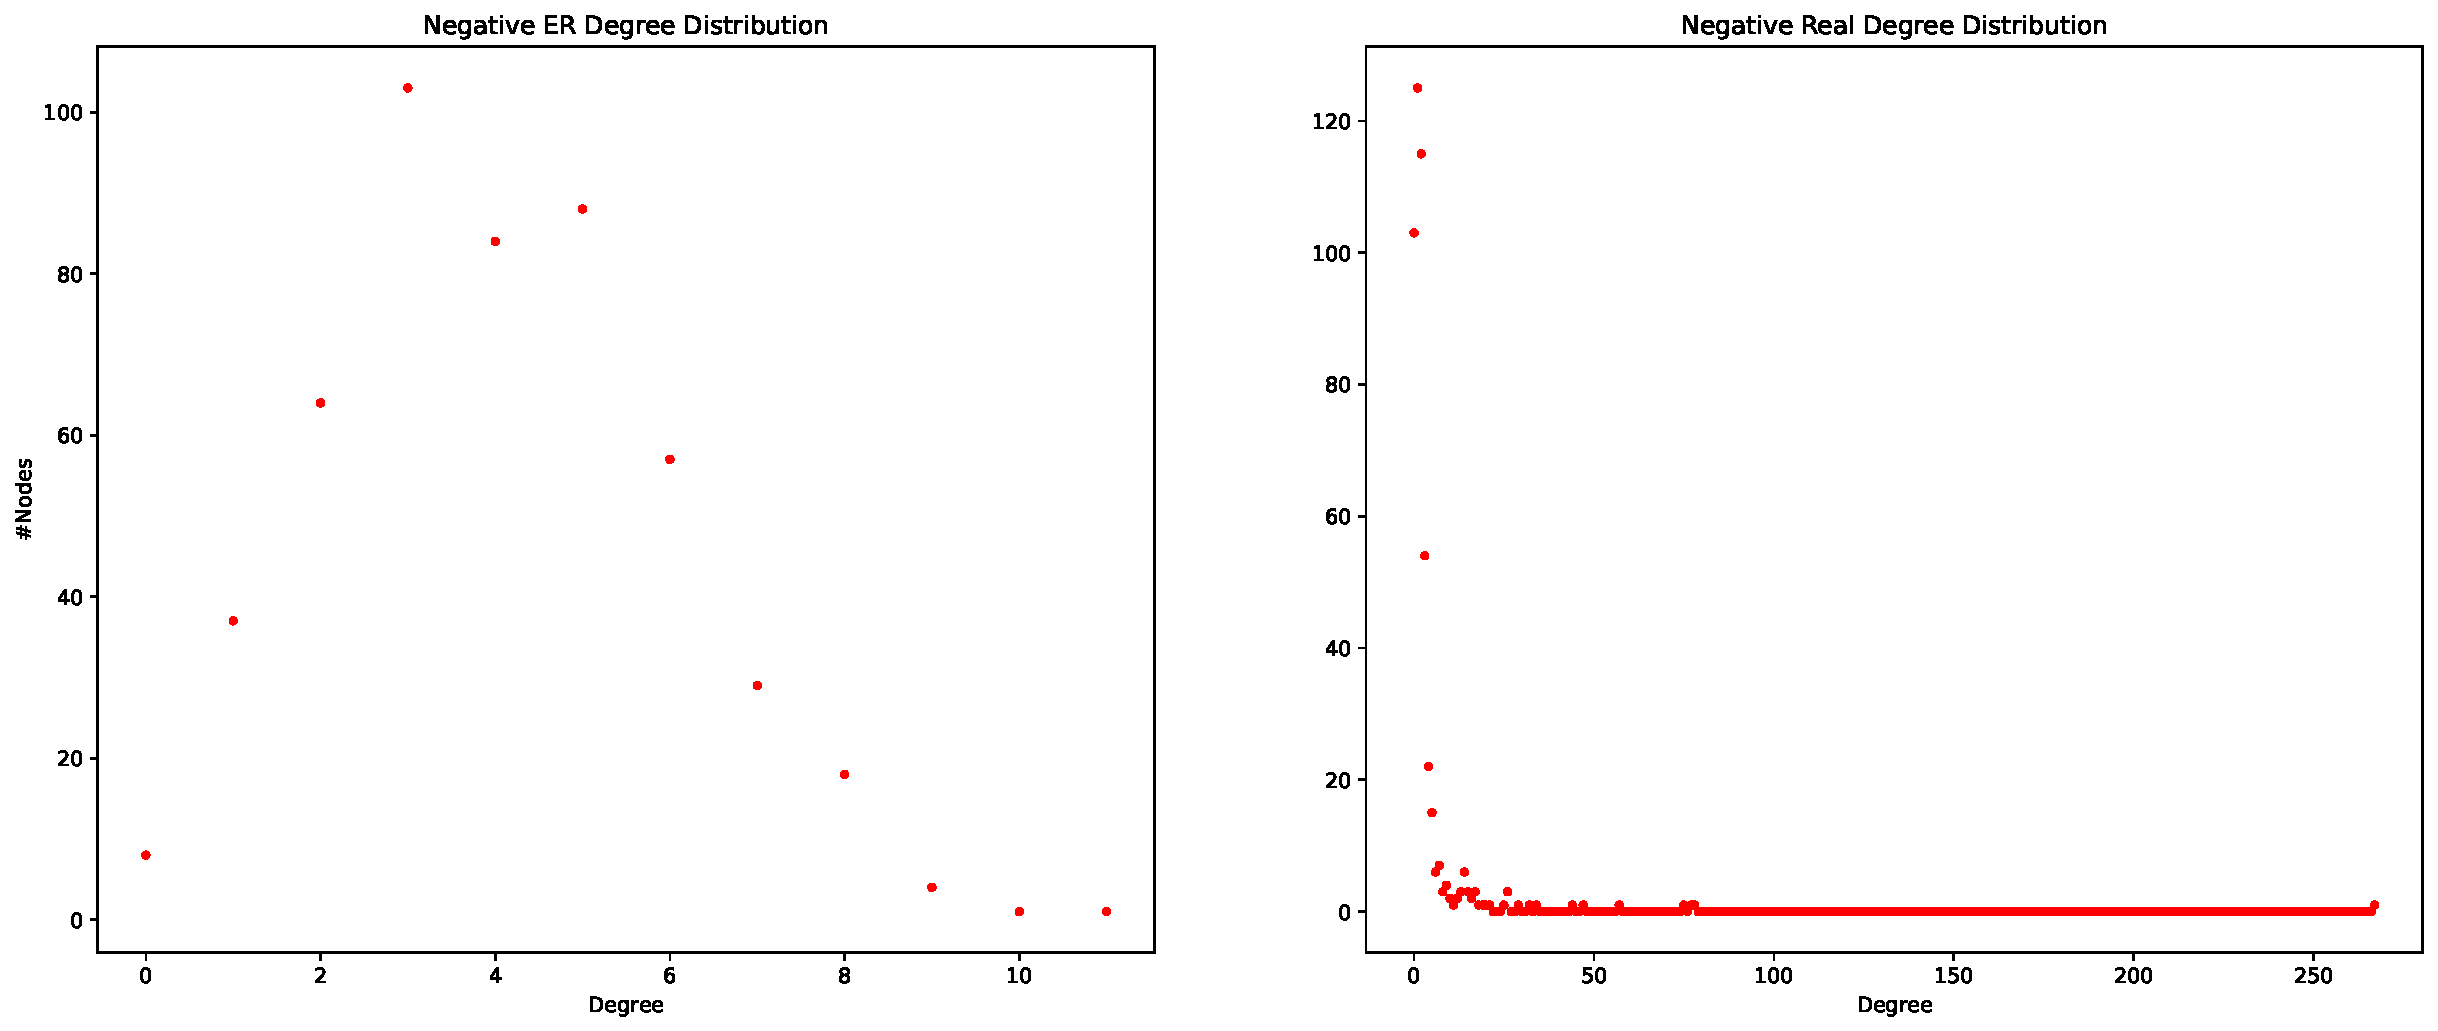
\includegraphics[width=\linewidth]{plot/er_comparison_negative.pdf}
	\caption{Negative ER Degree Distribution}
\end{figure}
\subsubsection{Comparision with BA}
A BA graph having same nodes and edges of our positive and negative graphs need $m$(number of edges to attach) = 143 for positive, 2 for negative. Fitting degree distribution with a powerlaw we obtained for positive: $\alpha_{BA} = 5.29 \pm 0.41$, $\alpha_{Real} = 15.38 \pm 5.06$, for negative: $\alpha_{BA} = 3.67 \pm 0.20$, $\alpha_{Real} = 7.05 \pm 0.31$, BA graph with this parameters is not an appropriate model for our graphs as well.
\begin{figure}[h]
	\centering
	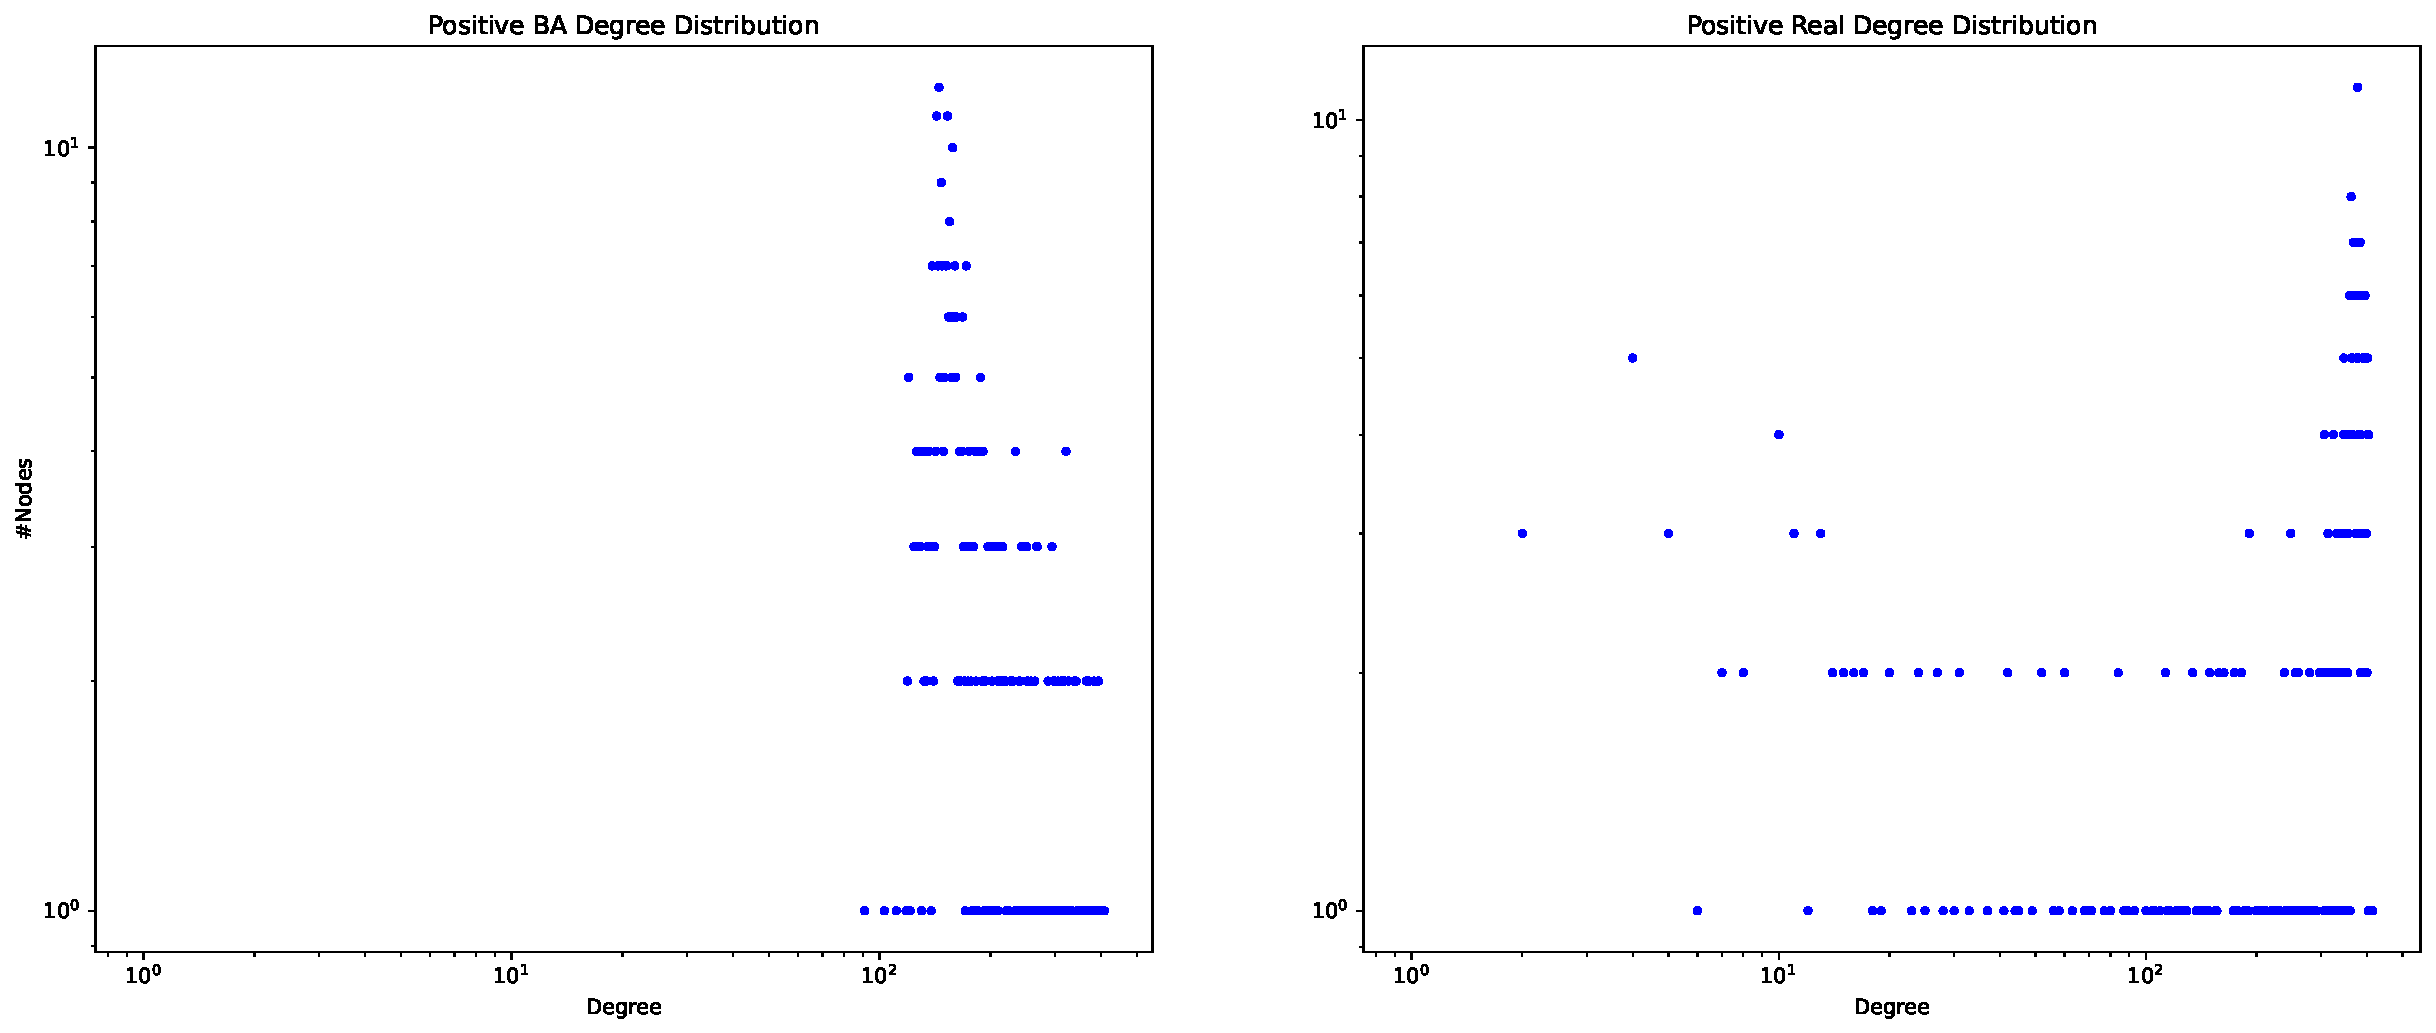
\includegraphics[width=\linewidth]{plot/ba_comparison_positive.pdf}
	\caption{Positive BA Degree Distribution}
\end{figure}
\begin{figure}[h]
	\centering
	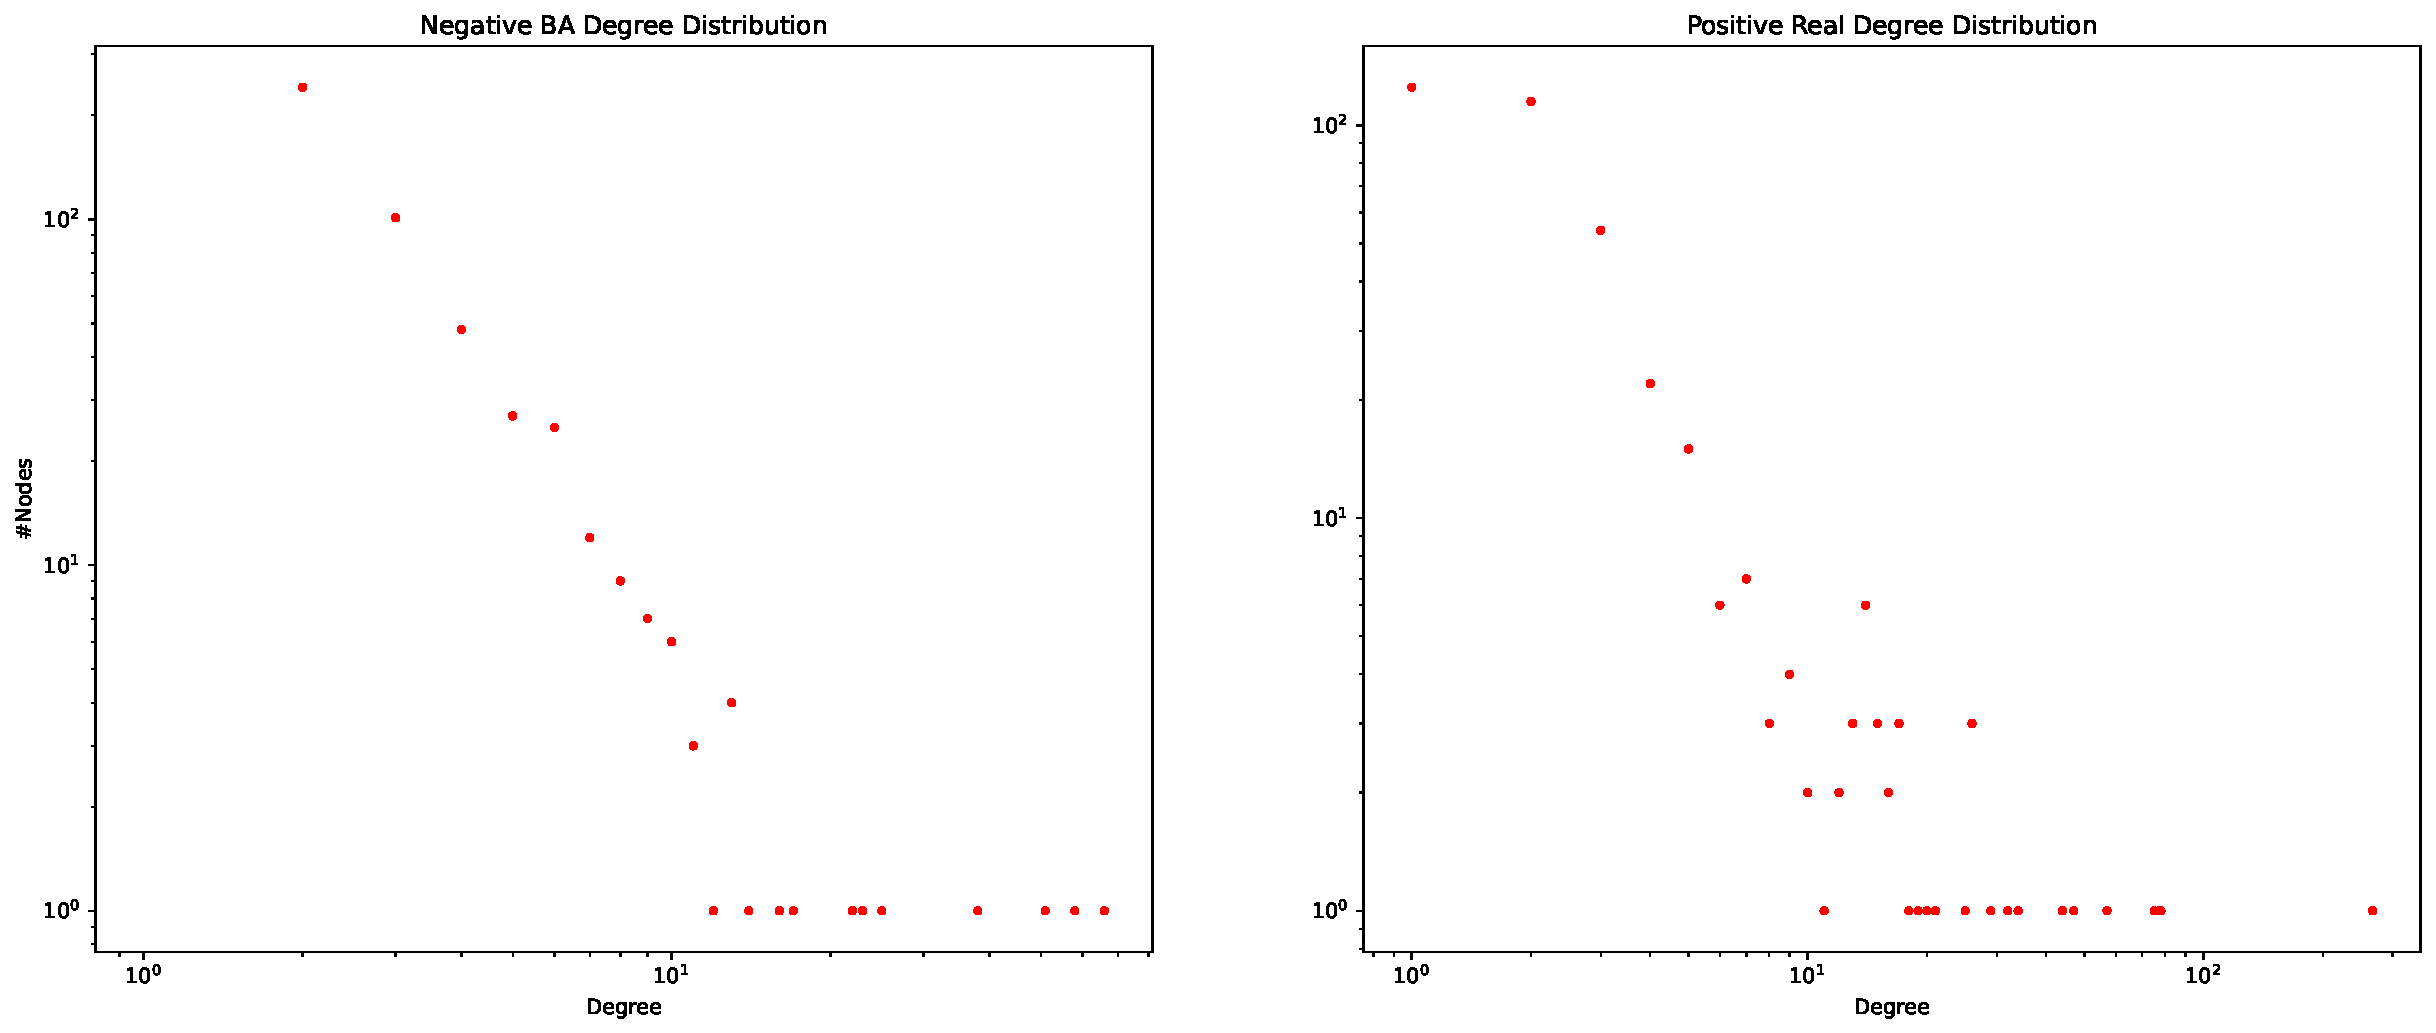
\includegraphics[width=\linewidth]{plot/ba_comparison_negative.pdf}
	\caption{Negative BA Degree Distribution}
\end{figure}
\subsubsection{Closeness centrality}
By evaluating closeness centrality we obtained the following results: positive graph closeness values are higher than negative one, considering the 20 largest values of closeness for positive and negative, we noticed that $30\%$ of stocks belongs to Industrial sector for positive and $30\%$ belongs to Information Technology for negative.
\begin{figure}[h]
	\centering
	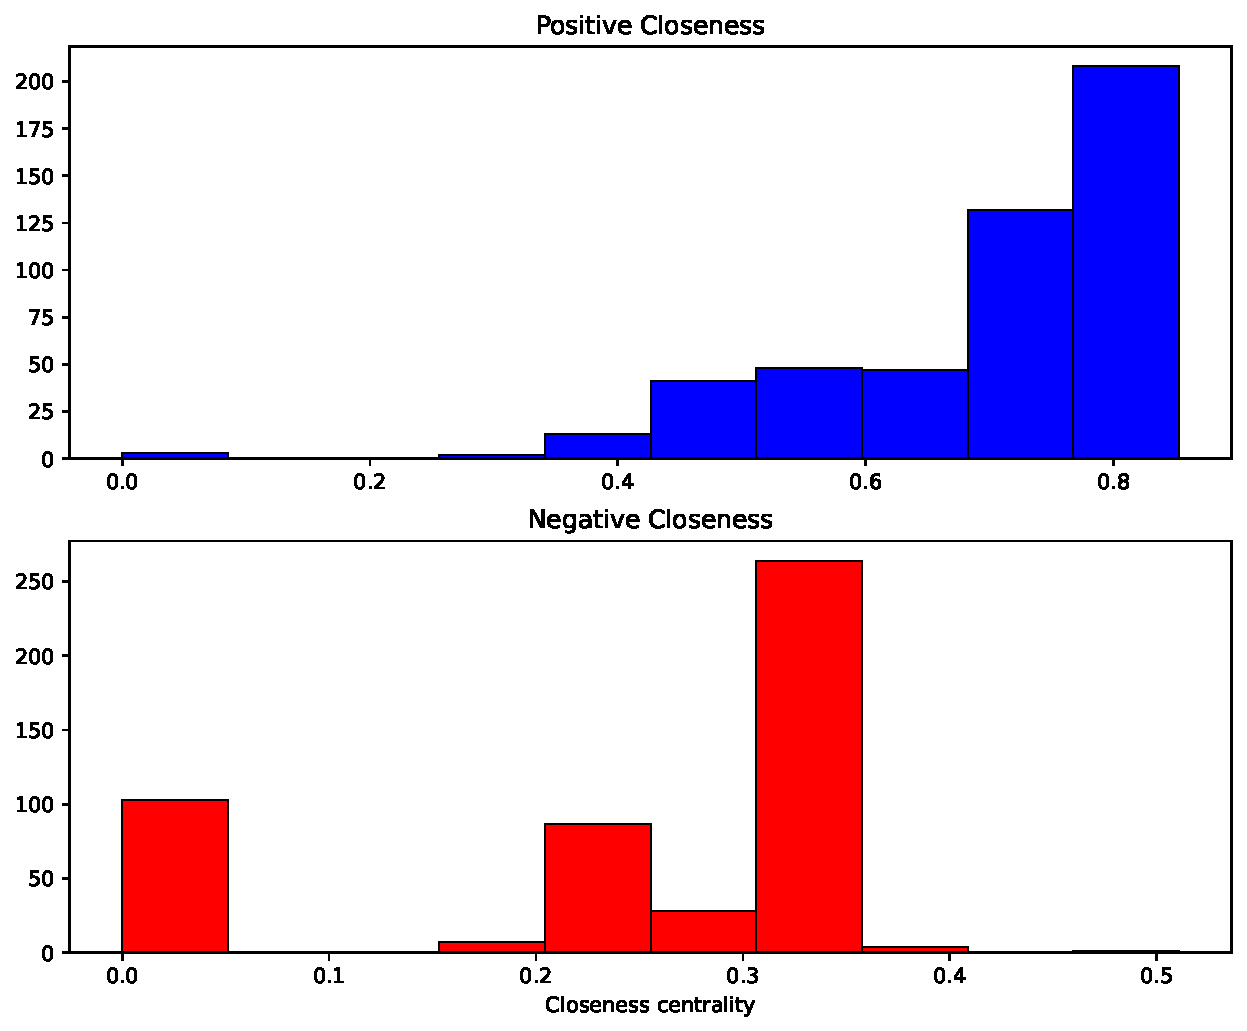
\includegraphics[width=\linewidth]{plot/distribution_closeness.pdf}
	\caption{Distribution Closeness}
\end{figure}
\begin{figure}[h]
	\centering
	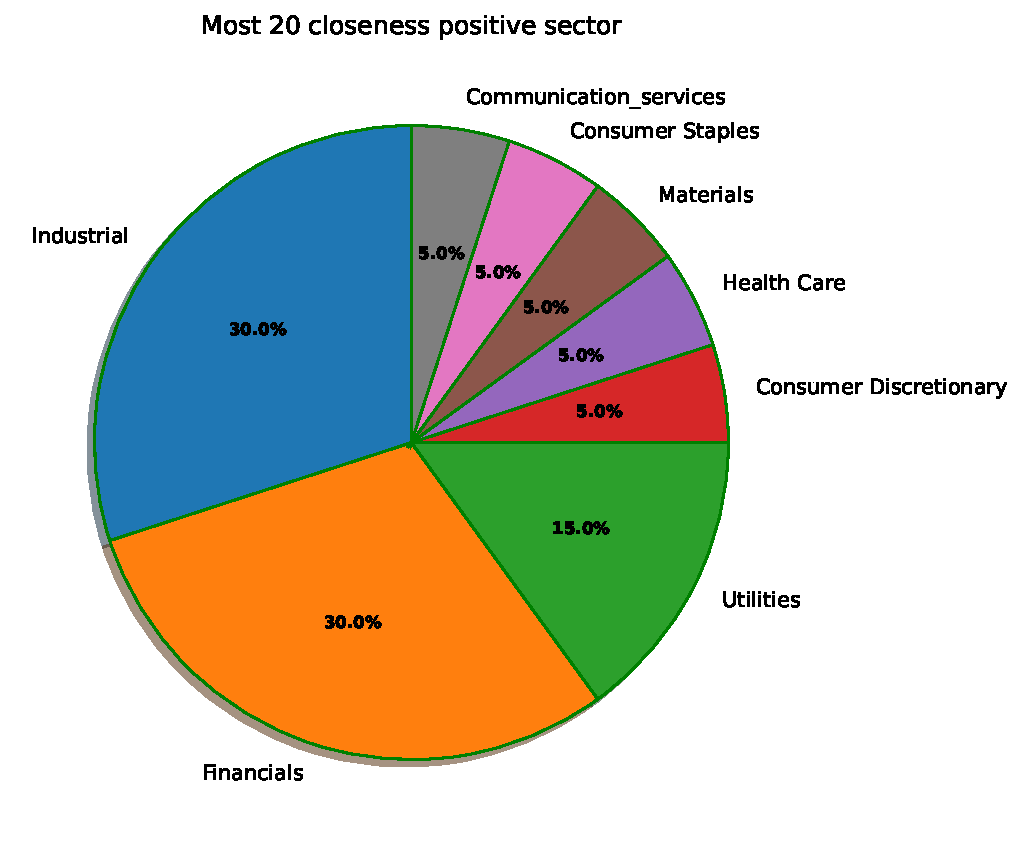
\includegraphics[width=0.65\linewidth]{plot/pie_clos_pos.pdf}
\end{figure}
\begin{figure}[h]
	\centering
	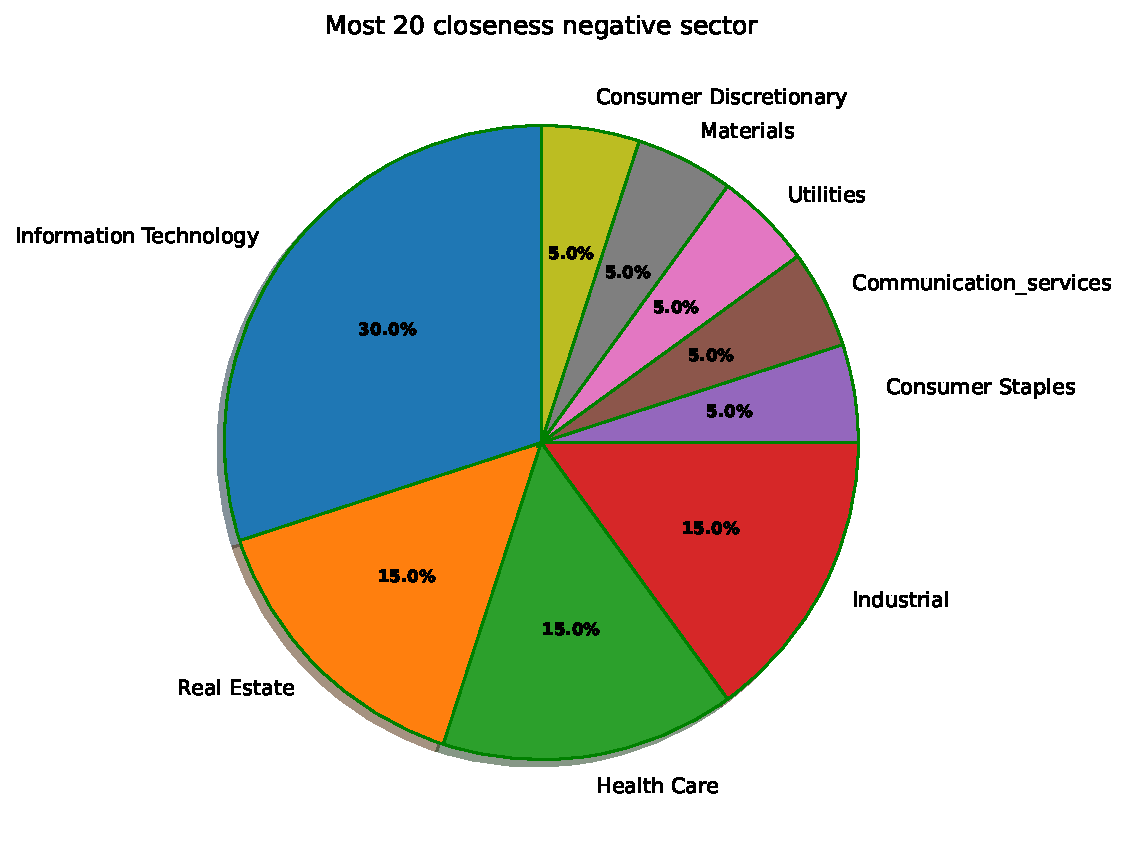
\includegraphics[width=0.65\linewidth]{plot/pie_clos_neg.pdf}
	\caption{Pie Chart Closeness}
\end{figure}
\begin{figure}[h]
	\centering
	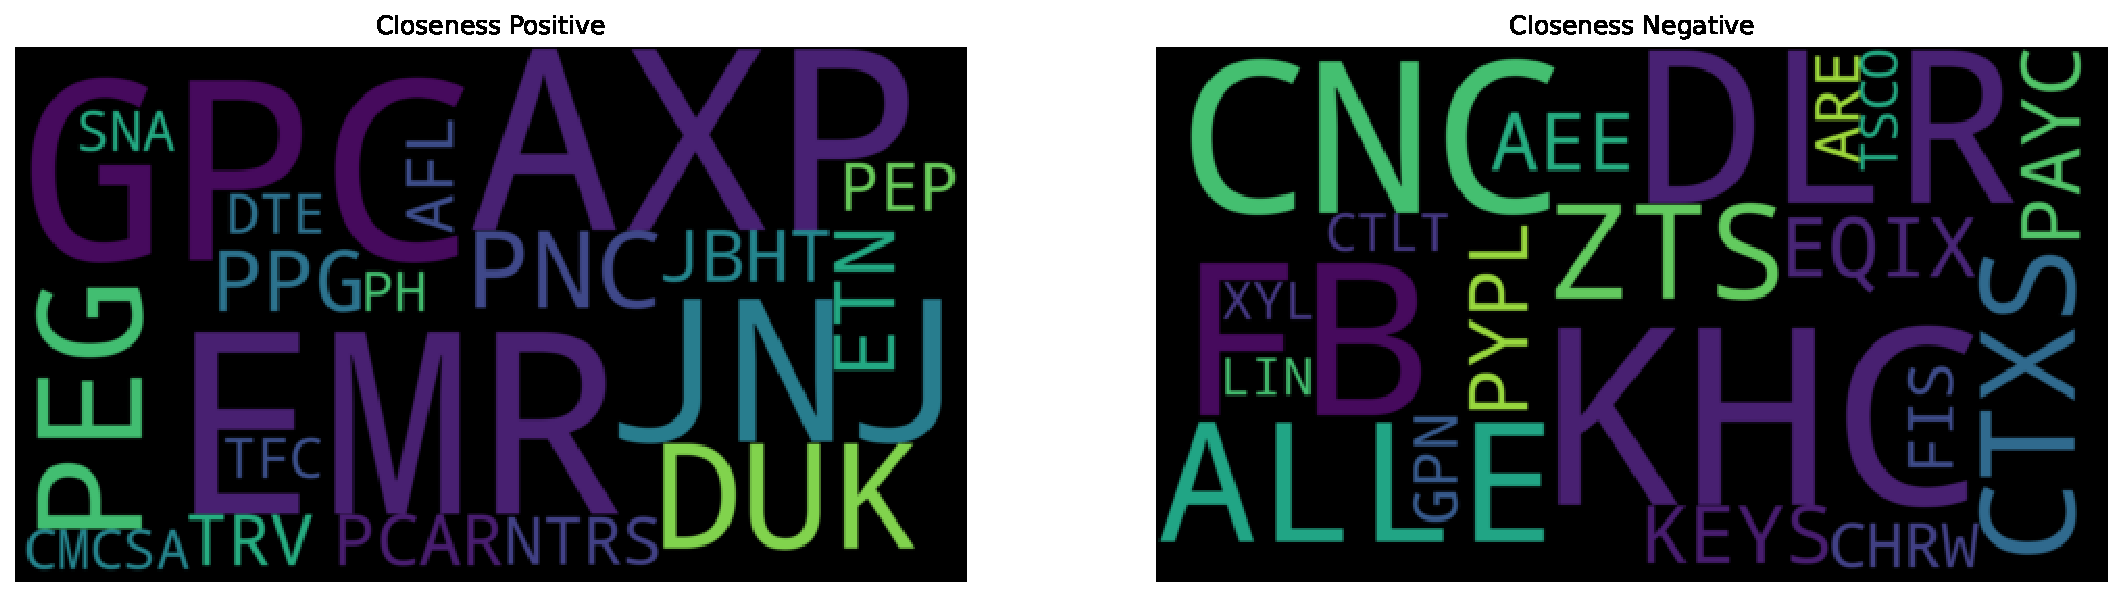
\includegraphics[width= \linewidth]{plot/wordcloud_closeness.pdf}
	\caption{Wordcloud Closeness}
\end{figure}
\subsubsection{Betweenness centrality}
Evaluating betweenness centrality we obtained the follow results: most values for positive are nearly 0.0025 and 0.05 for negative, these small values are due the absence of meaningful bridges in the graph; considering the biggest 20 values we noticed as $30\%$ of stocks belongs to Financials sector for positive and $25\%$ belongs to Information Technology for negative.
\begin{figure}[h]
	\centering
	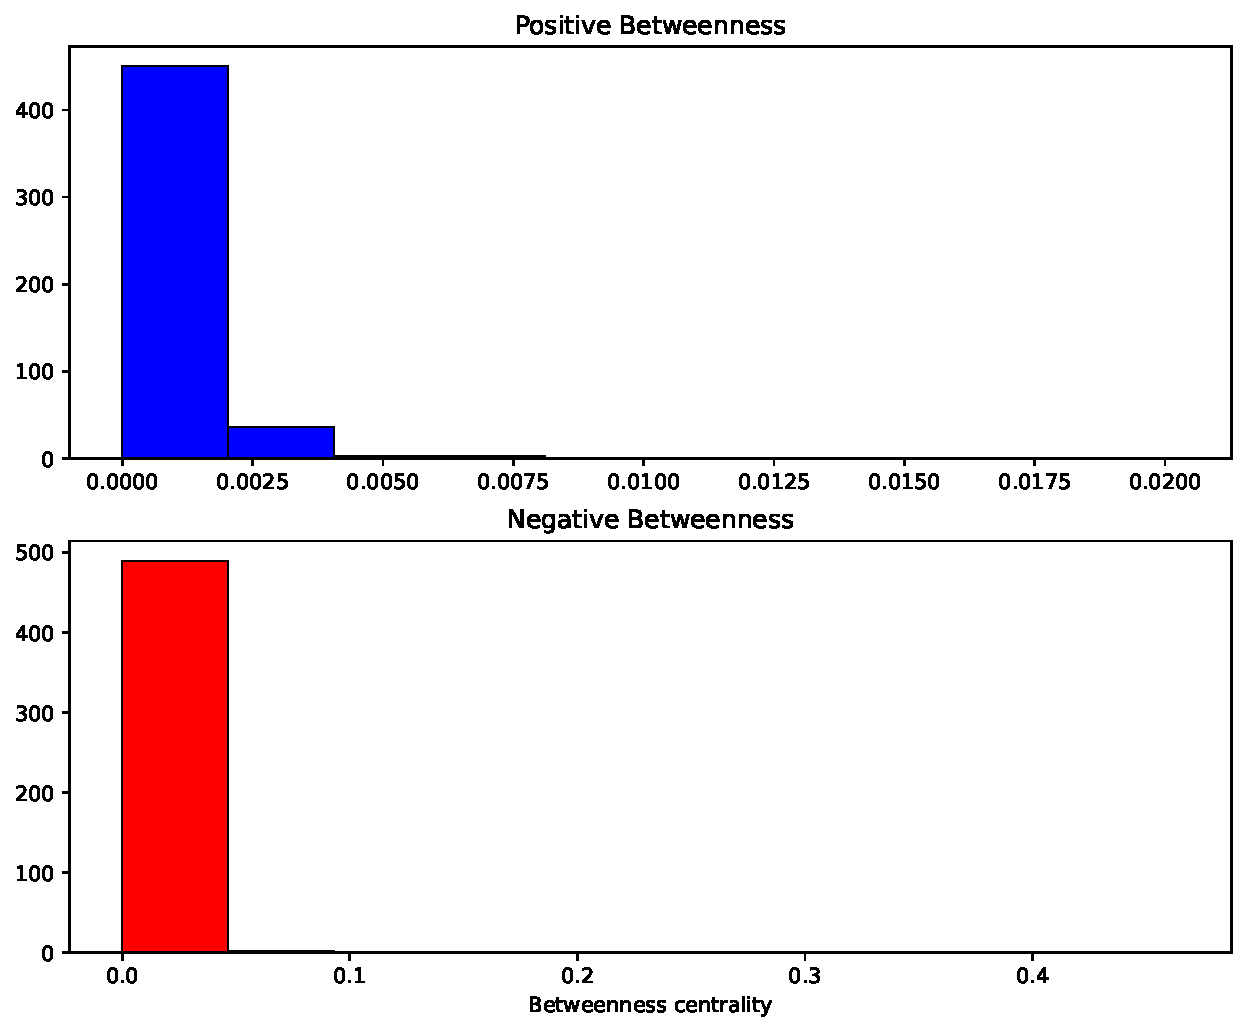
\includegraphics[width=\linewidth]{plot/distribution_betweenness.pdf}
	\caption{Distribution Betweenness}
\end{figure}
\begin{figure}[h]
	\centering
	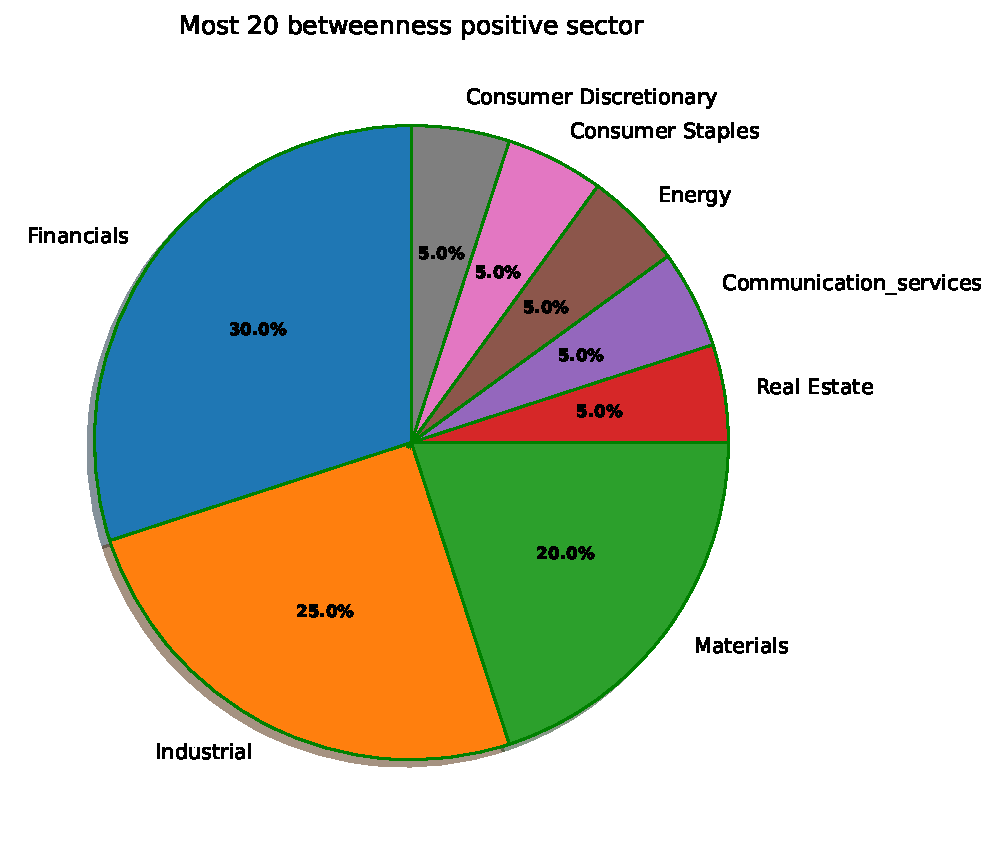
\includegraphics[width=0.65\linewidth]{plot/pie_bet_pos.pdf}
\end{figure}
\begin{figure}[h]
	\centering
	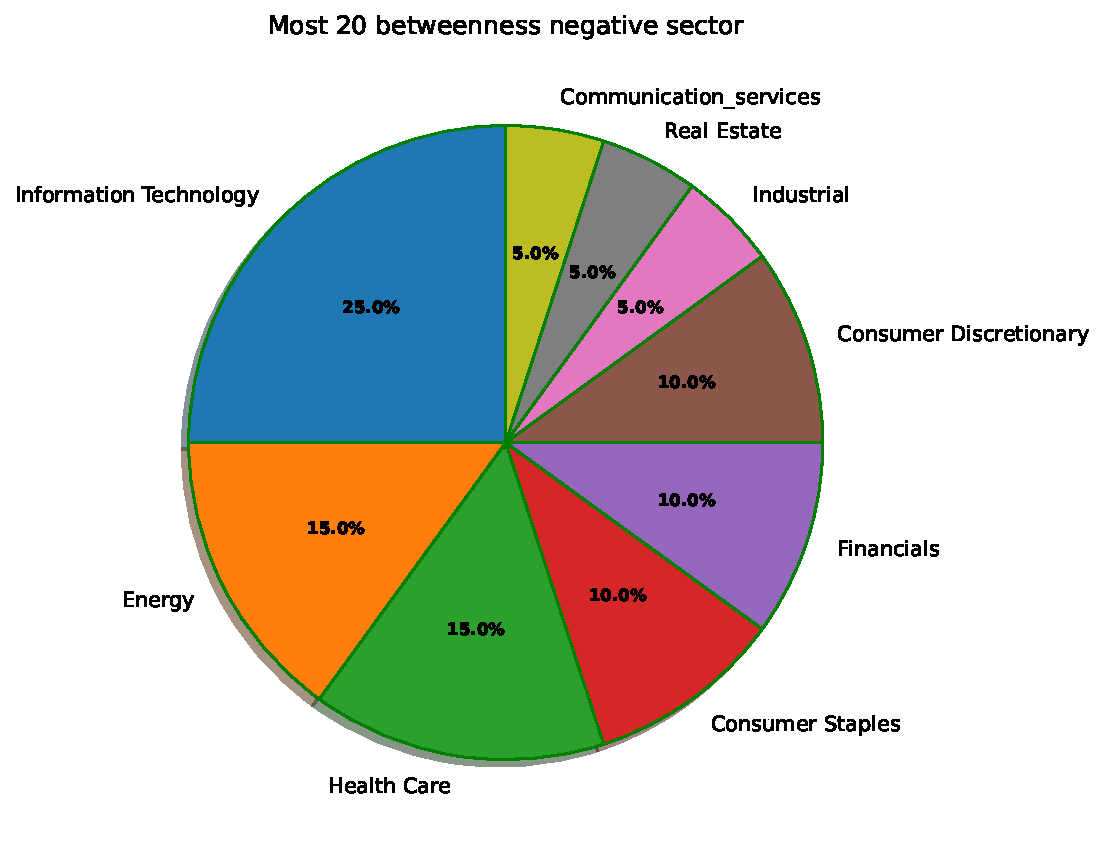
\includegraphics[width=0.65\linewidth]{plot/pie_bet_neg.pdf}
	\caption{Pie Chart Betweenness}
\end{figure}
Evaluating pagerank, considering the biggest 20 values we noticed as $30\%$ of stocks belongs to Financials sector for positive and $25\%$ belongs to Energy for negative. This results show the great centrality of the financial sector in stock market.
\begin{figure}[H]
	\centering
	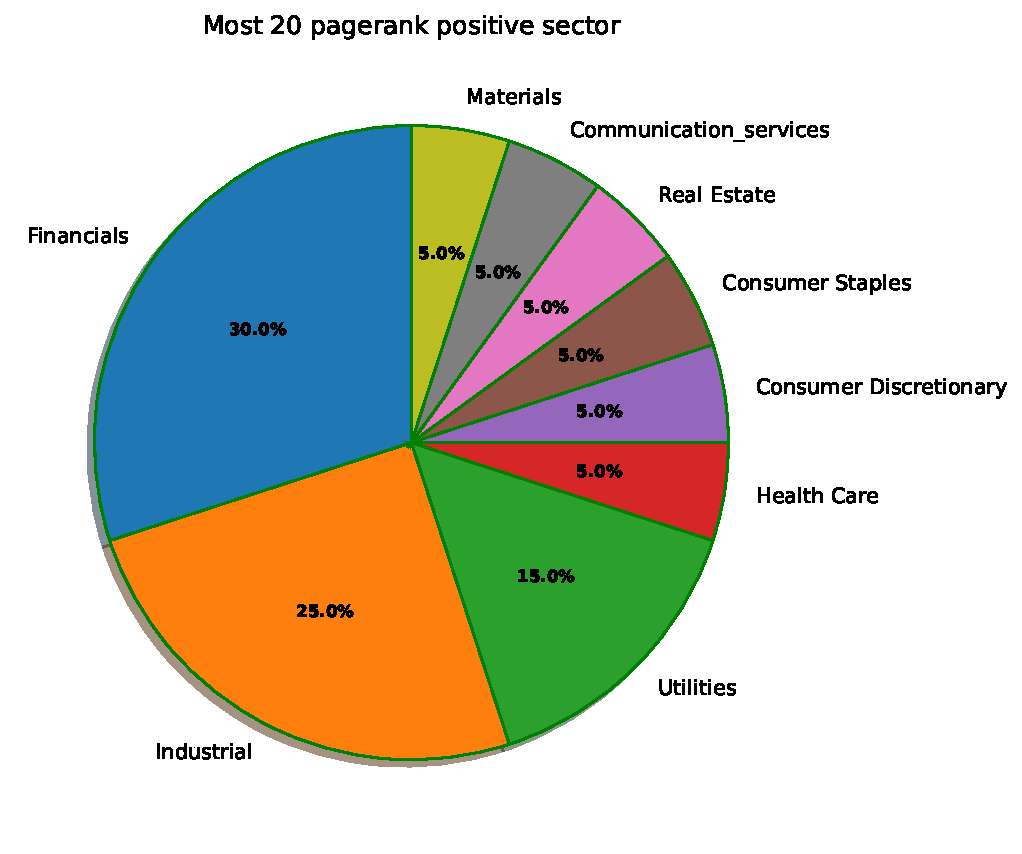
\includegraphics[width=0.65\linewidth]{plot/pie_page_pos.pdf}
\end{figure}
\begin{figure}[H]
	\centering
	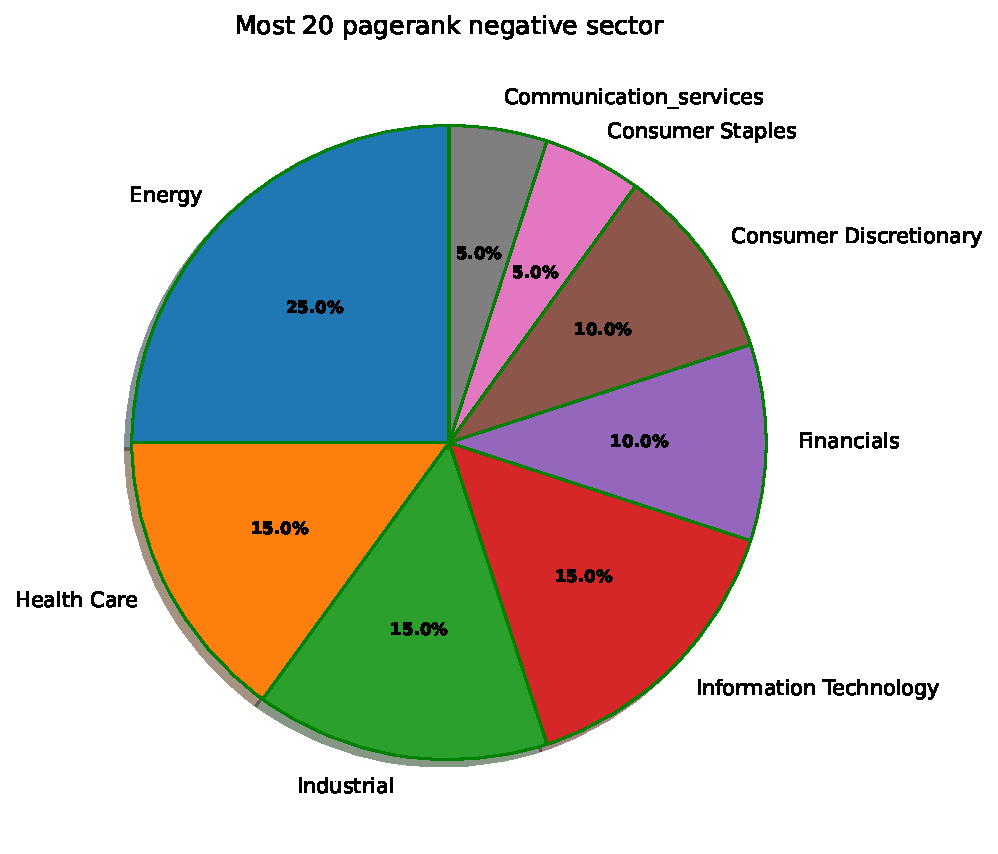
\includegraphics[width=0.65\linewidth]{plot/pie_page_neg.pdf}
	\caption{Pie Chart PageRank}
\end{figure}
\begin{figure}[H]
	\centering
	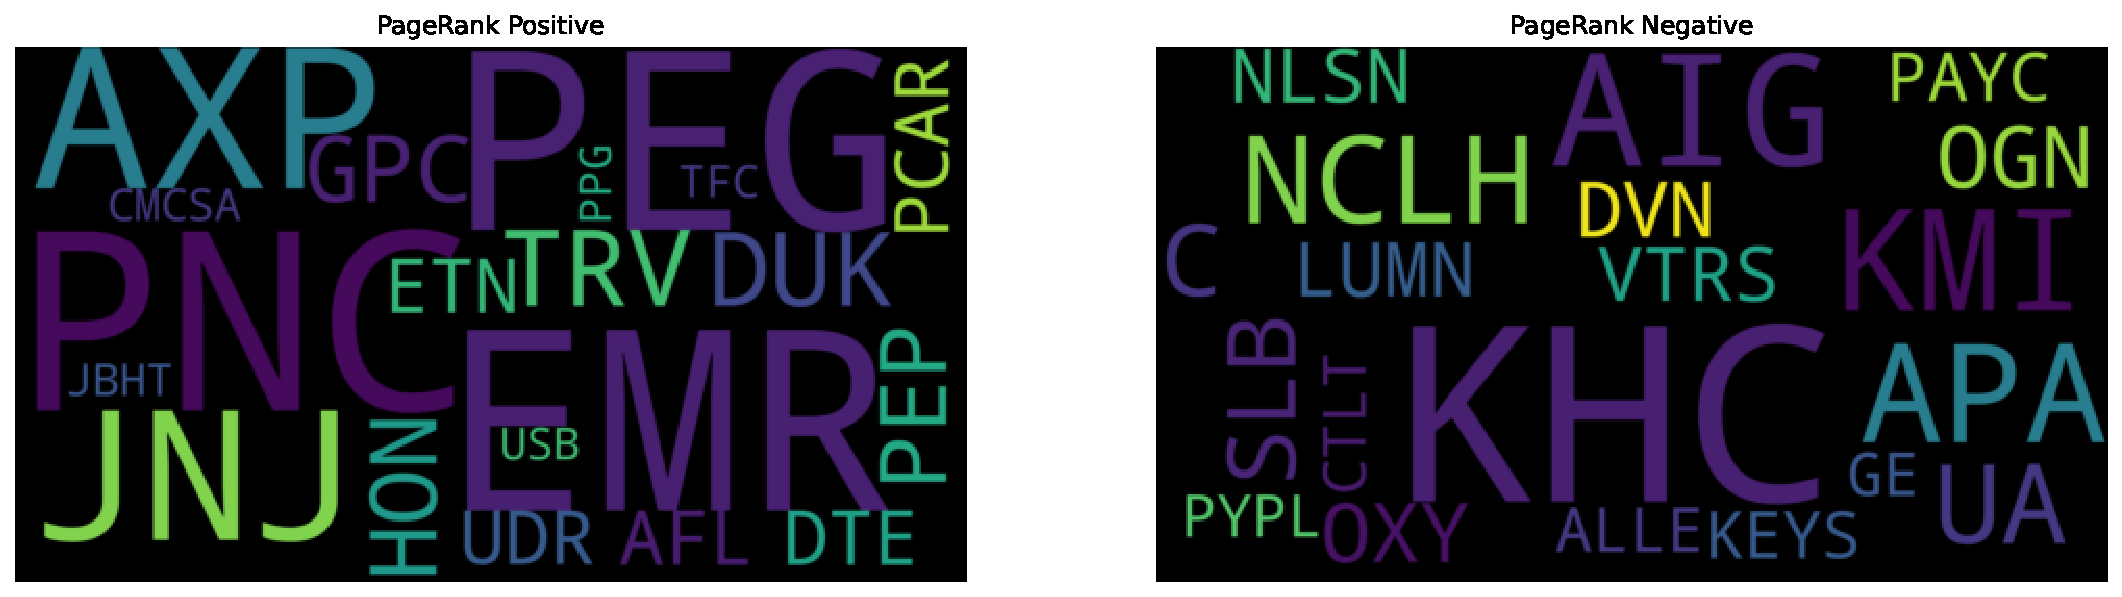
\includegraphics[width= \linewidth]{plot/wordcloud_pagerank.pdf}
	\caption{Wordcloud PageRank}
\end{figure}
\subsubsection{Assortativity measures}
Considering sectors, positive's assortativity is 0.01, while negative's assortativity is -0.08, both graphs do not show homophily behaviour.\\
Using comformity with a decay factor of 3, 35\% of the least 20 disassortative firms belong to Energy
\begin{figure}[H]
	\centering
	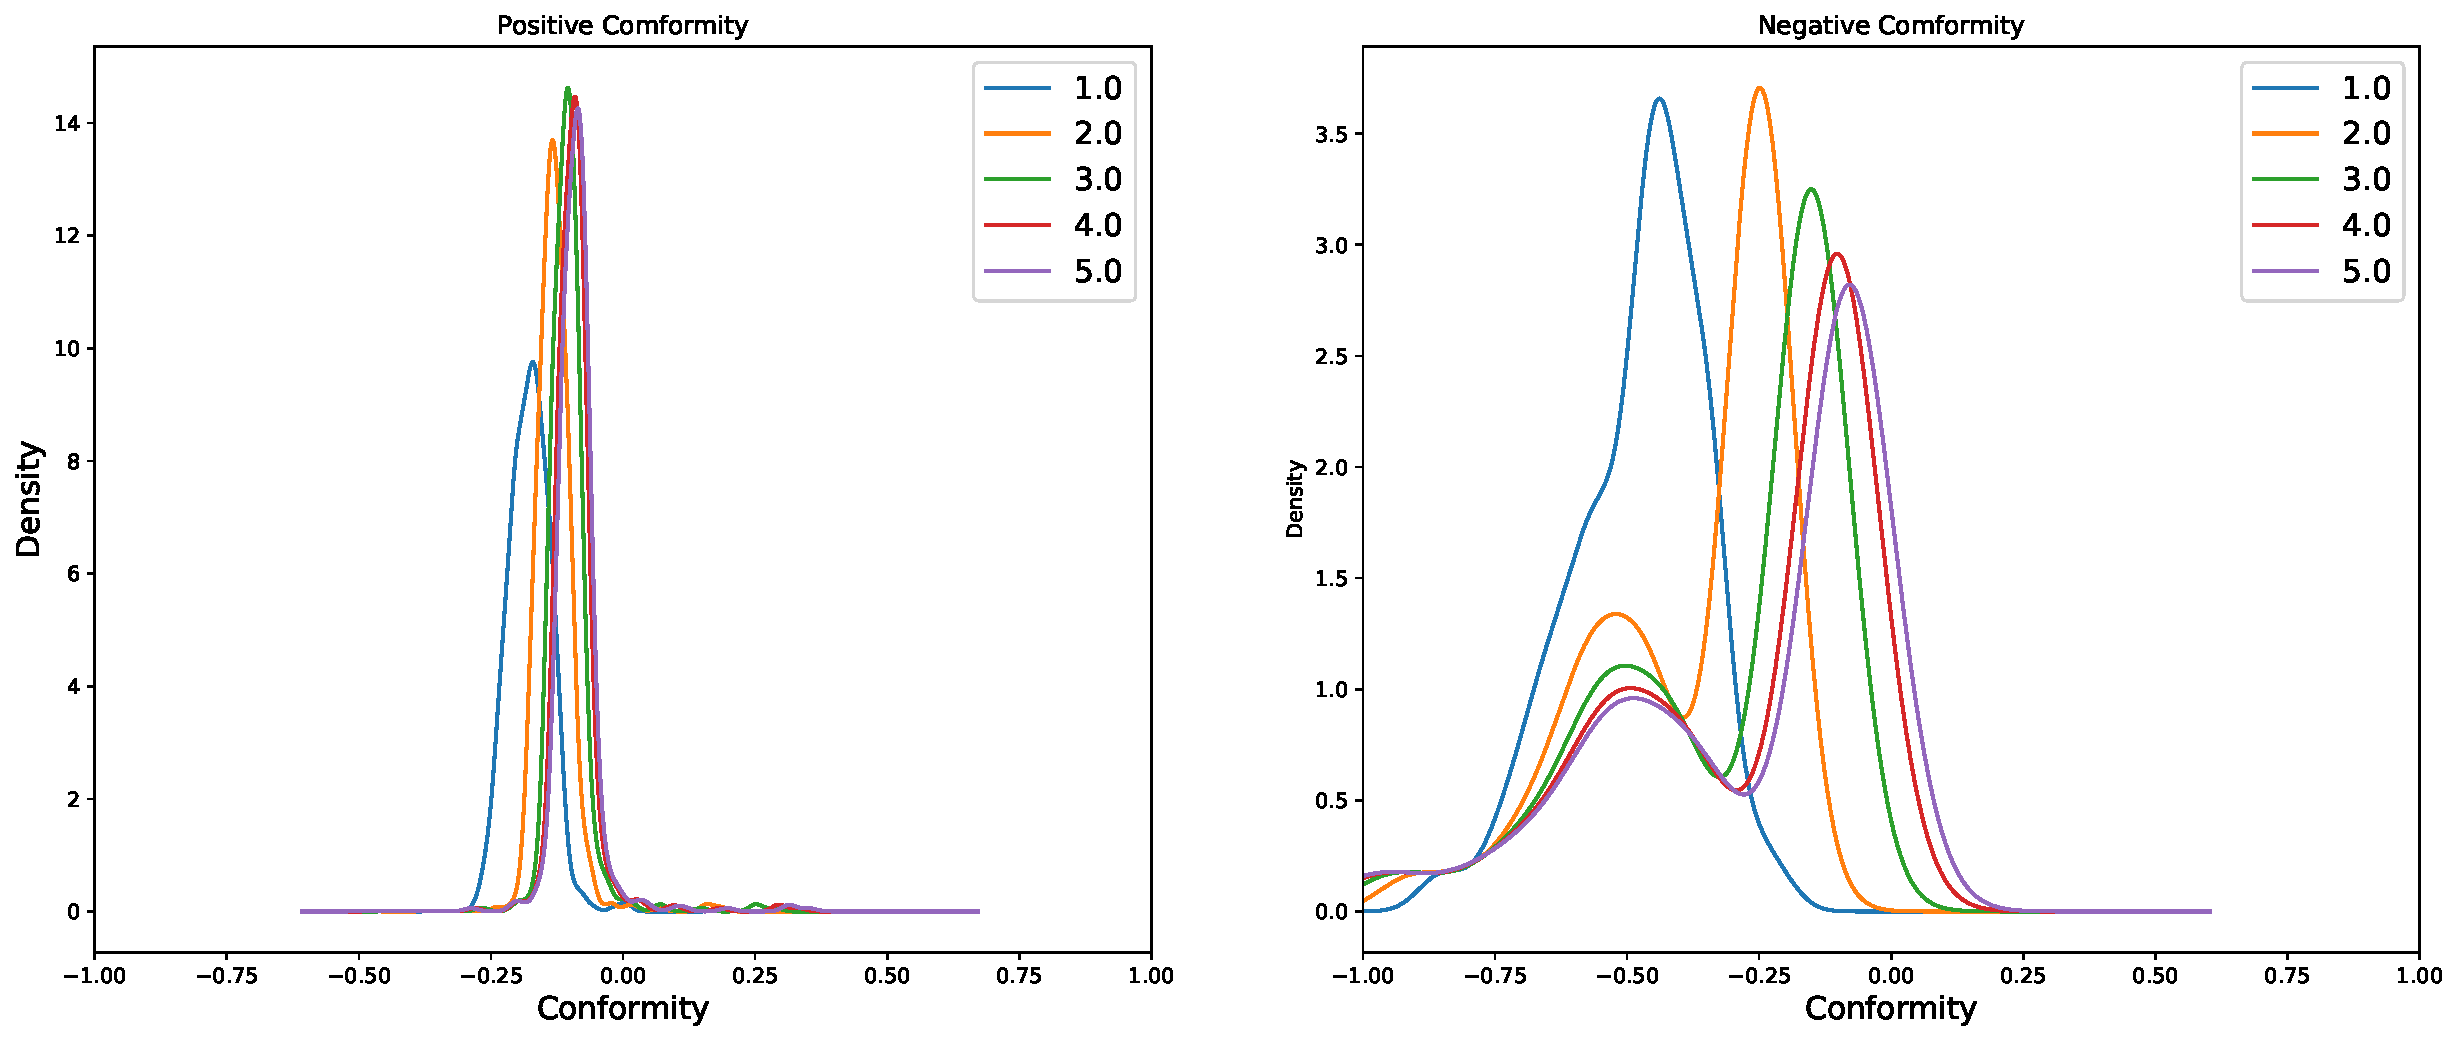
\includegraphics[width=\linewidth]{plot/comformity.pdf}
	\caption{Comformity at different decay values}
\end{figure}
\begin{figure}[H]
	\centering
	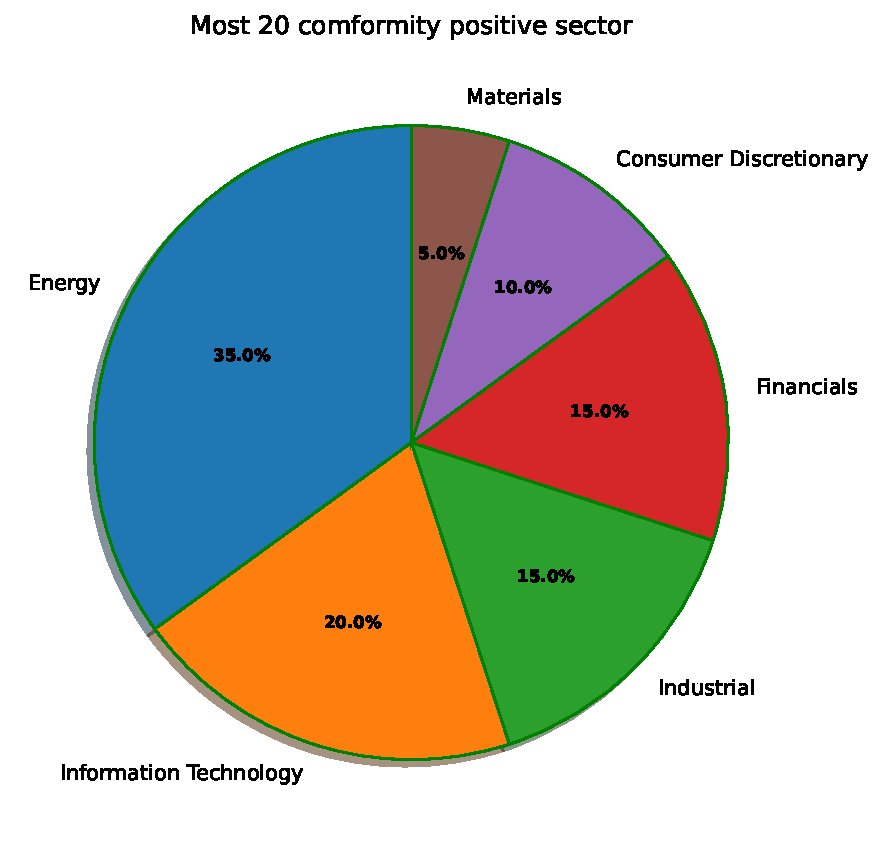
\includegraphics[width=0.65\linewidth]{plot/pie_comf_pos.pdf}
\end{figure}
\section{Task 1: Dynamic Network Analysis}
We built a dynamic graph considering 60 snapshots (from 1962 to 2021)
\begin{figure}[H]
	\centering
	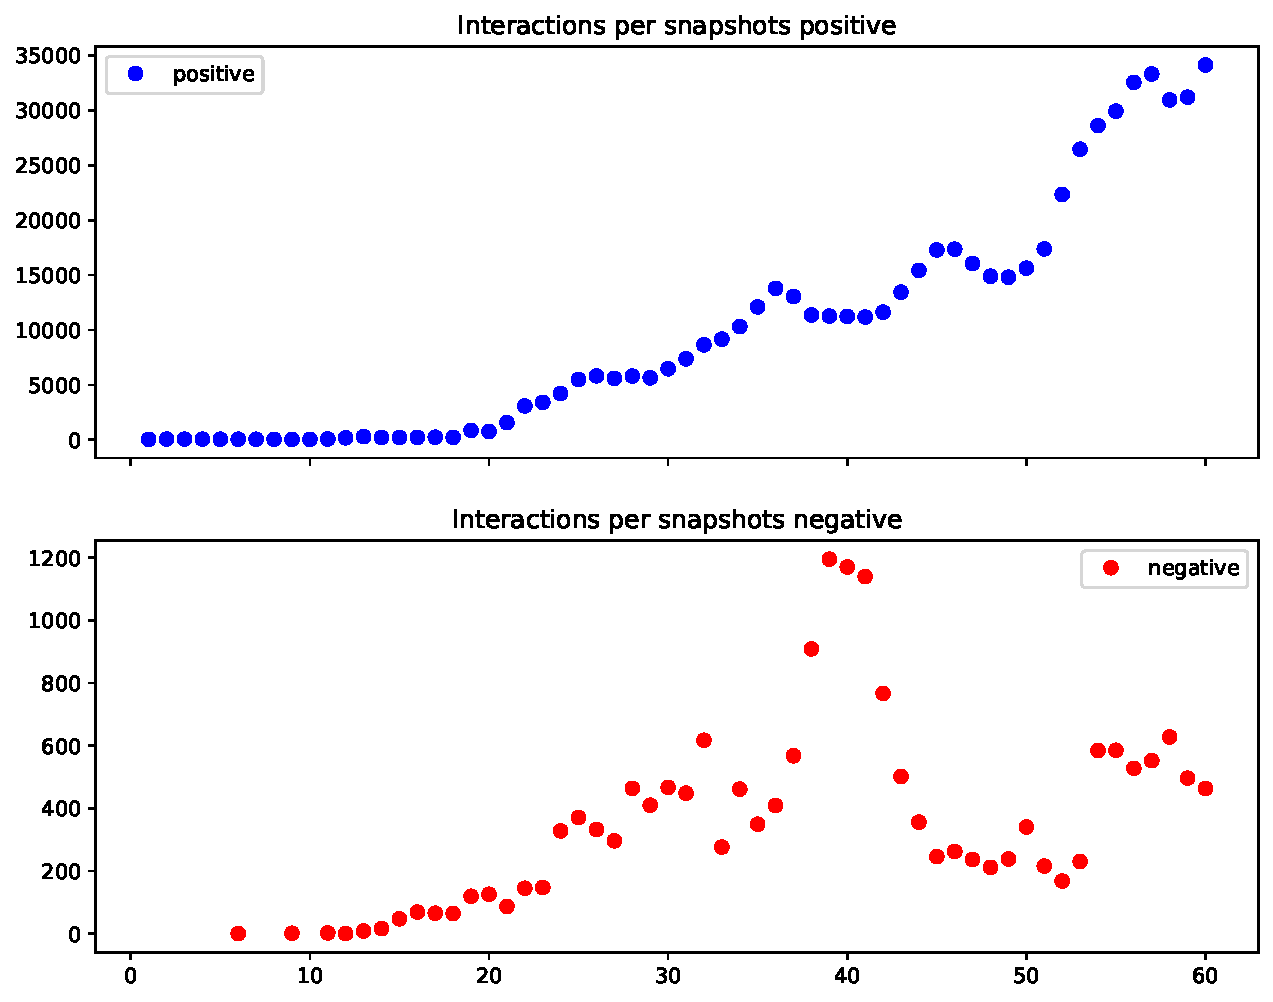
\includegraphics[width= \linewidth]{plot/inter_snap.pdf}
	\caption{Interaction per snapshots}
\end{figure}
Considering the interaction per snapshots values, positive graph tend to increase, while negative have an unstable behaviour.\\
Studying the distribution of degree over snapshot, we noticed that the degree distribution tends to stabilize, we fitted the degree distribution of the 60th snapshot of the negative graph with a power law ($Y = A +BX$, data are in logs) obtaining: $A = 3.98 \pm 0.34, B = -1.03 \pm 0.11, \chi^2 = 0.99, R2 = 0.74$. \\
Coverage for the positive graph is 0.55, while for the negative one is 0.50. By studying the contribution of each node in both graph, the top 3 nodes associated to the highest values in contribution belong to Energy sector for both graph.\\
The density of the positive graph tends to increase, albeit with significant fluctuations snapshot by snapshot, while that of the negative converges to 0.  
\begin{figure}[H]
	\centering
	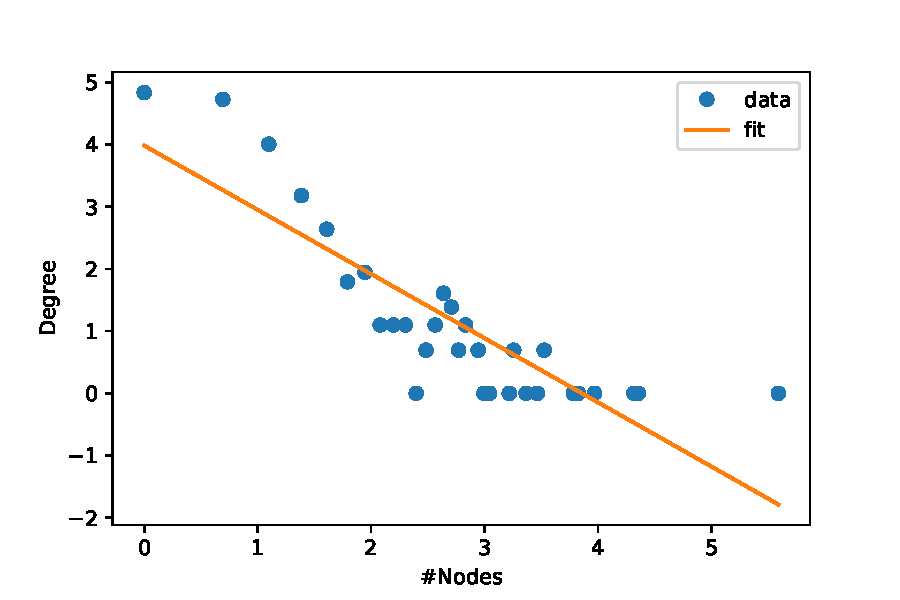
\includegraphics[width= \linewidth]{plot/60_snap_fit_degree_neg_dist.pdf}
	\caption{Fit 60th snapshot negative degree distribution}
\end{figure}
\begin{figure}[H]
	\centering
	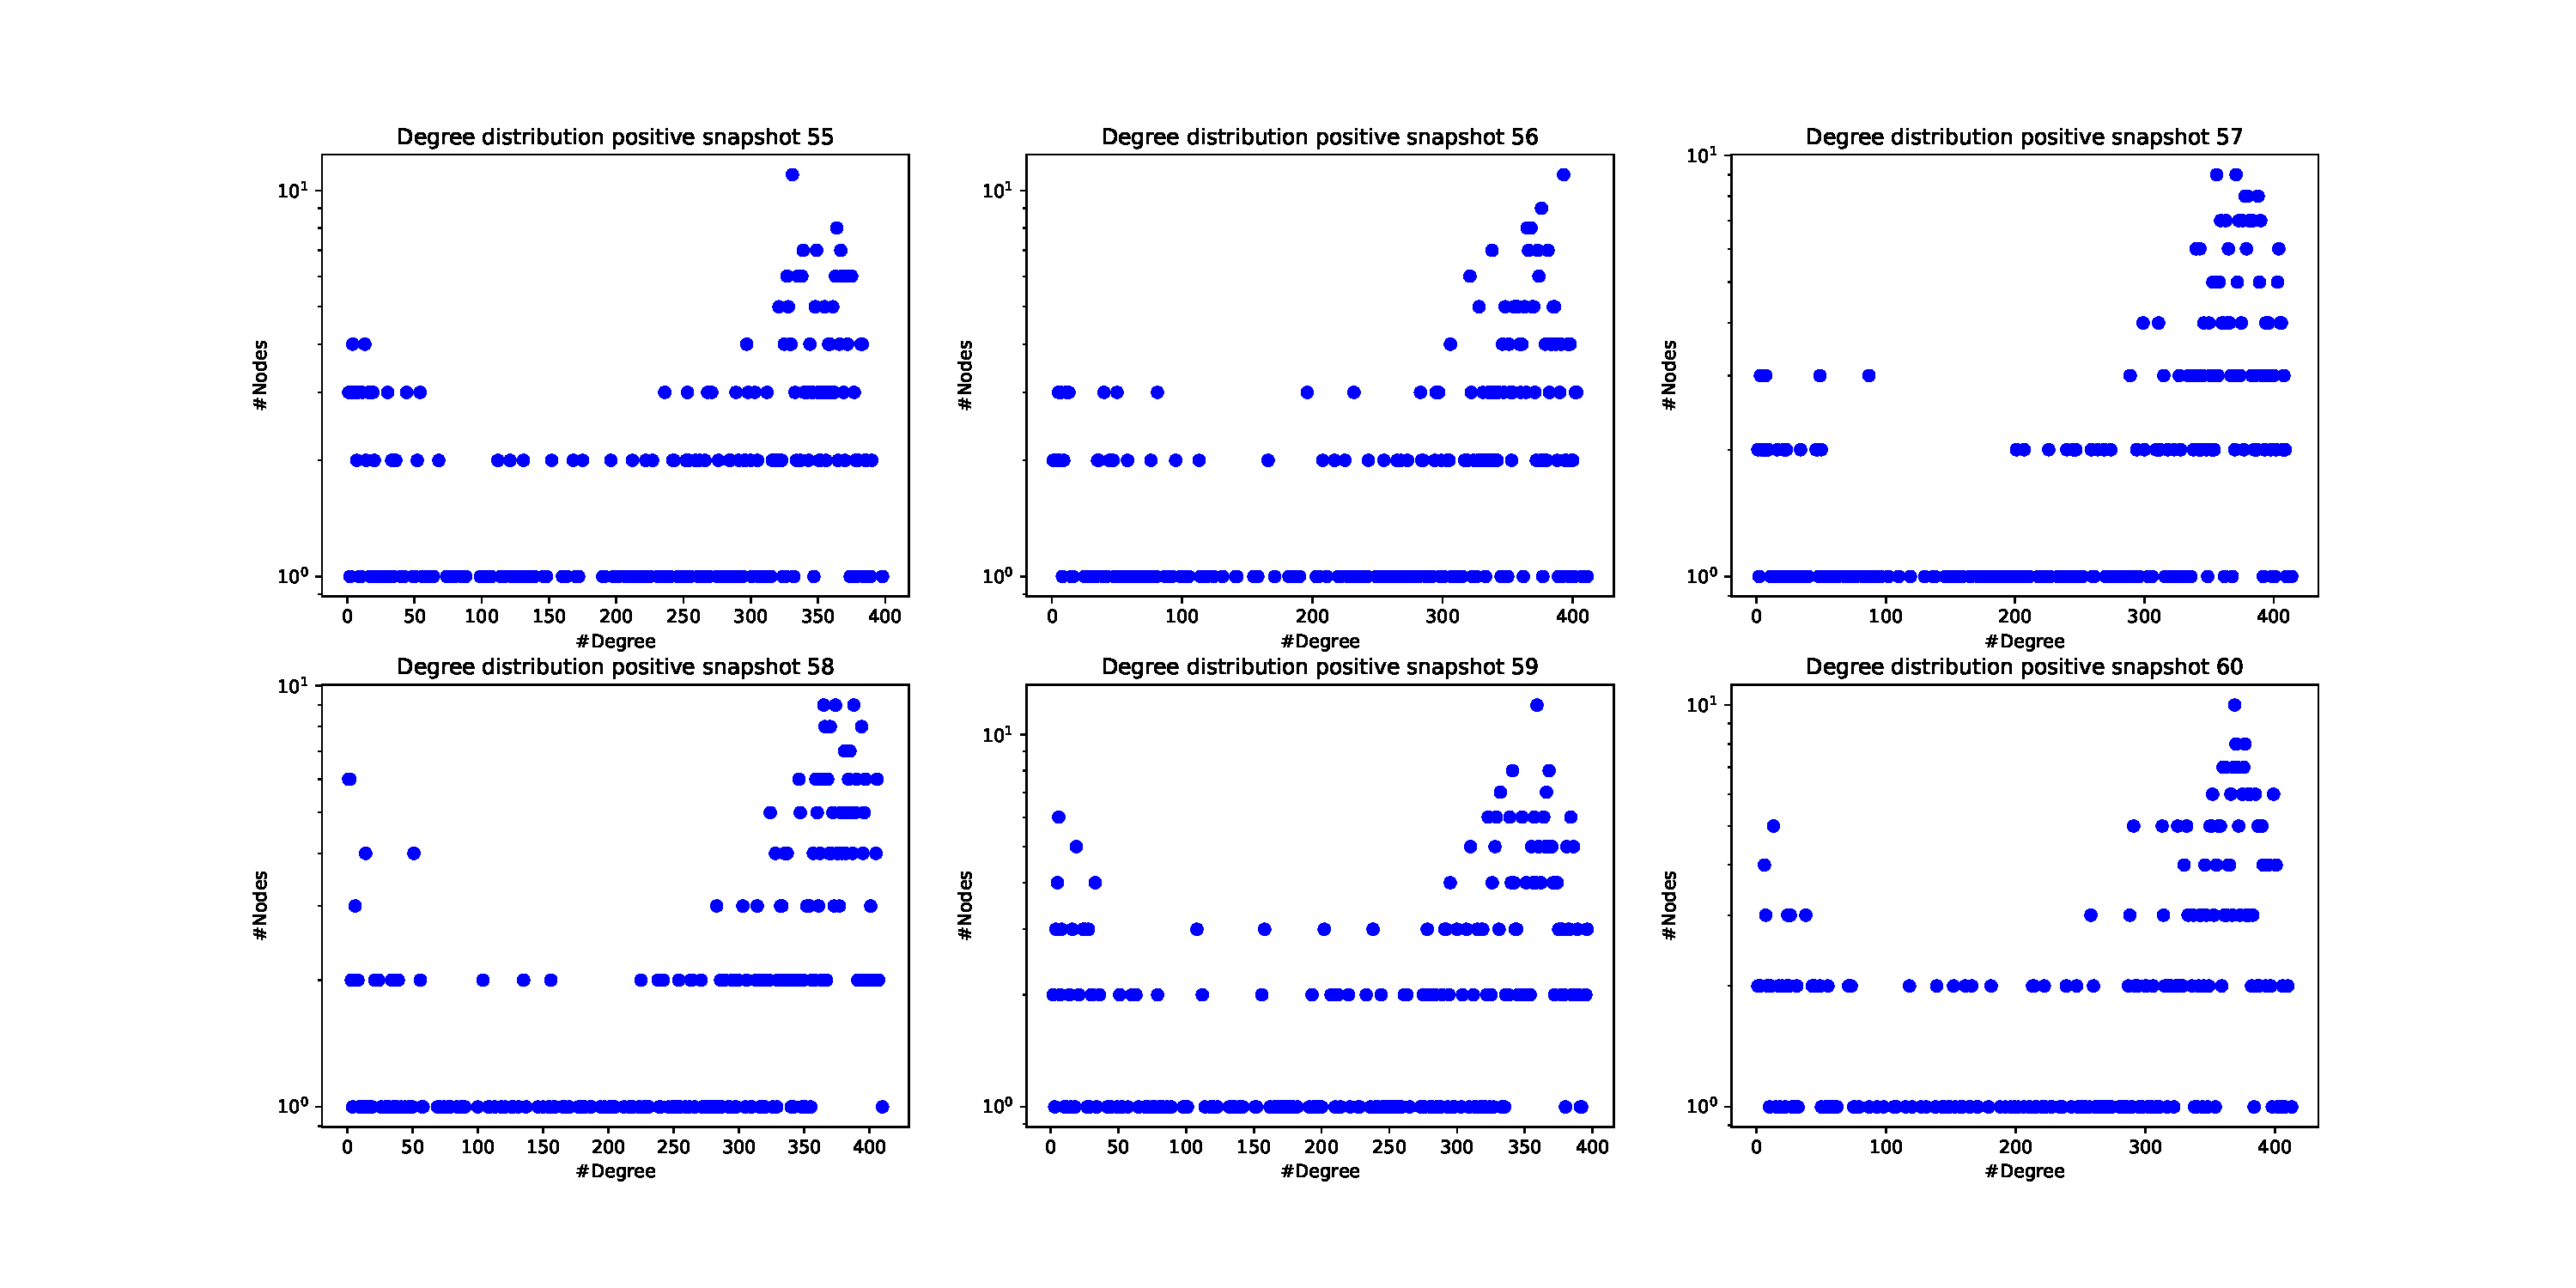
\includegraphics[width= \linewidth]{plot/first_10_snap_degree_pos_dist.pdf}
	\caption{Snapshot positive degree distribution}
\end{figure}
\begin{figure}[H]
	\centering
	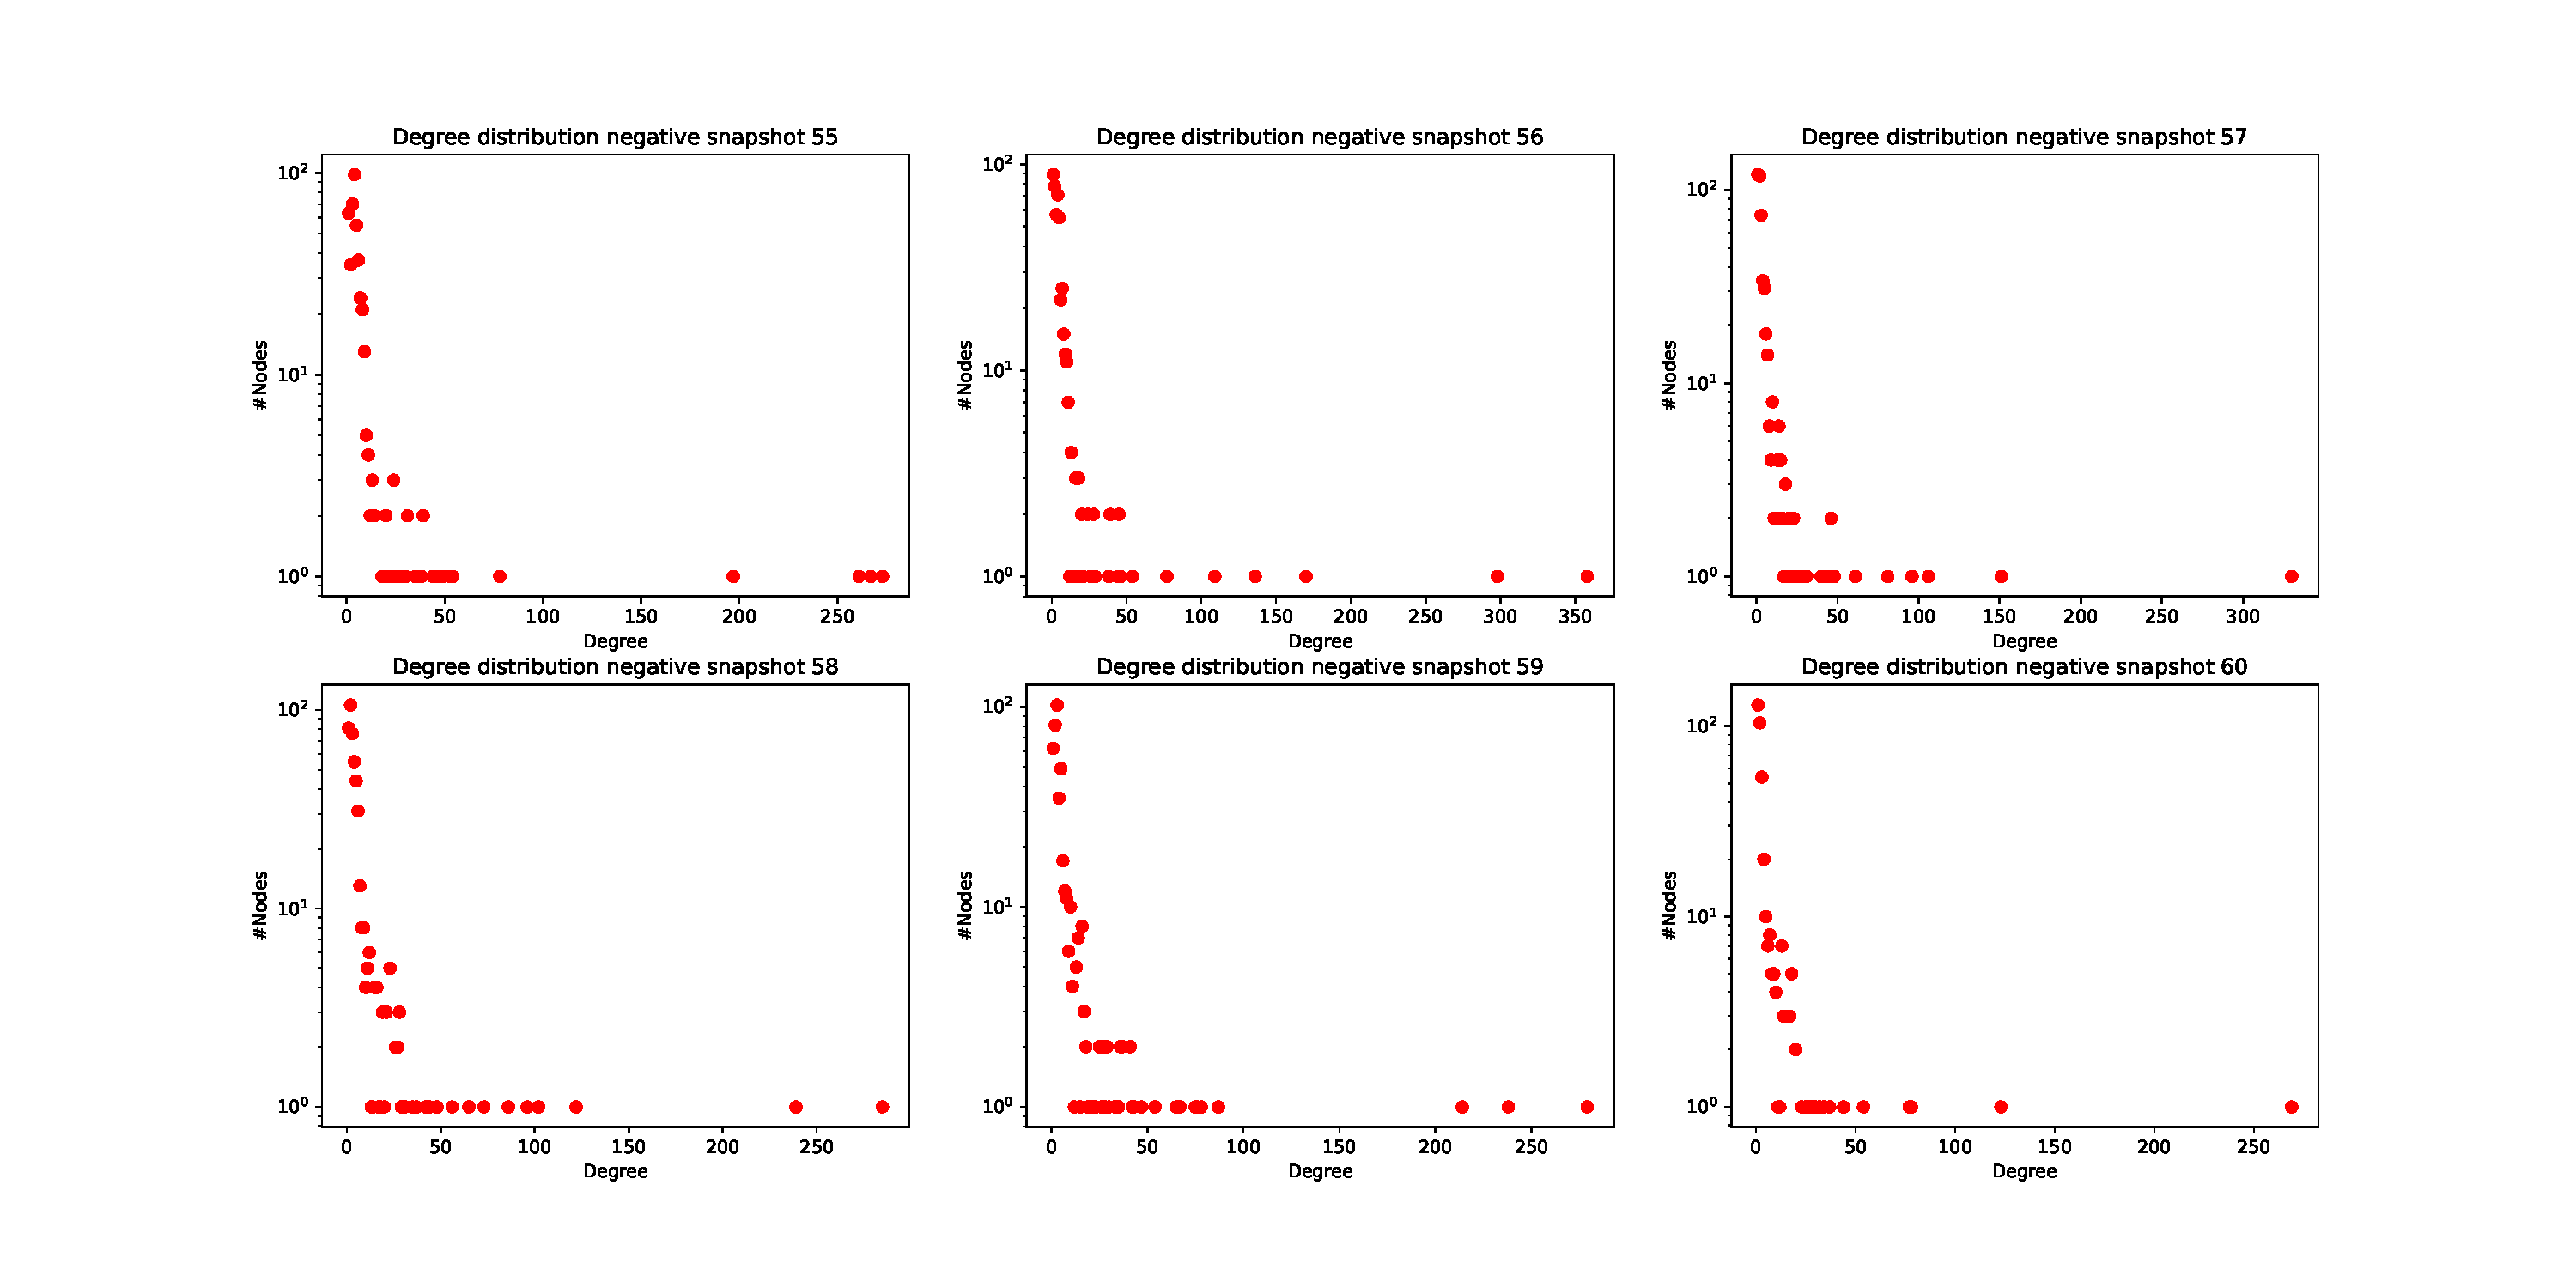
\includegraphics[width= \linewidth]{plot/first_10_snap_degree_neg_dist.pdf}
	\caption{Snapshot negative degree distribution}
\end{figure}
\begin{figure}[H]
	\centering
	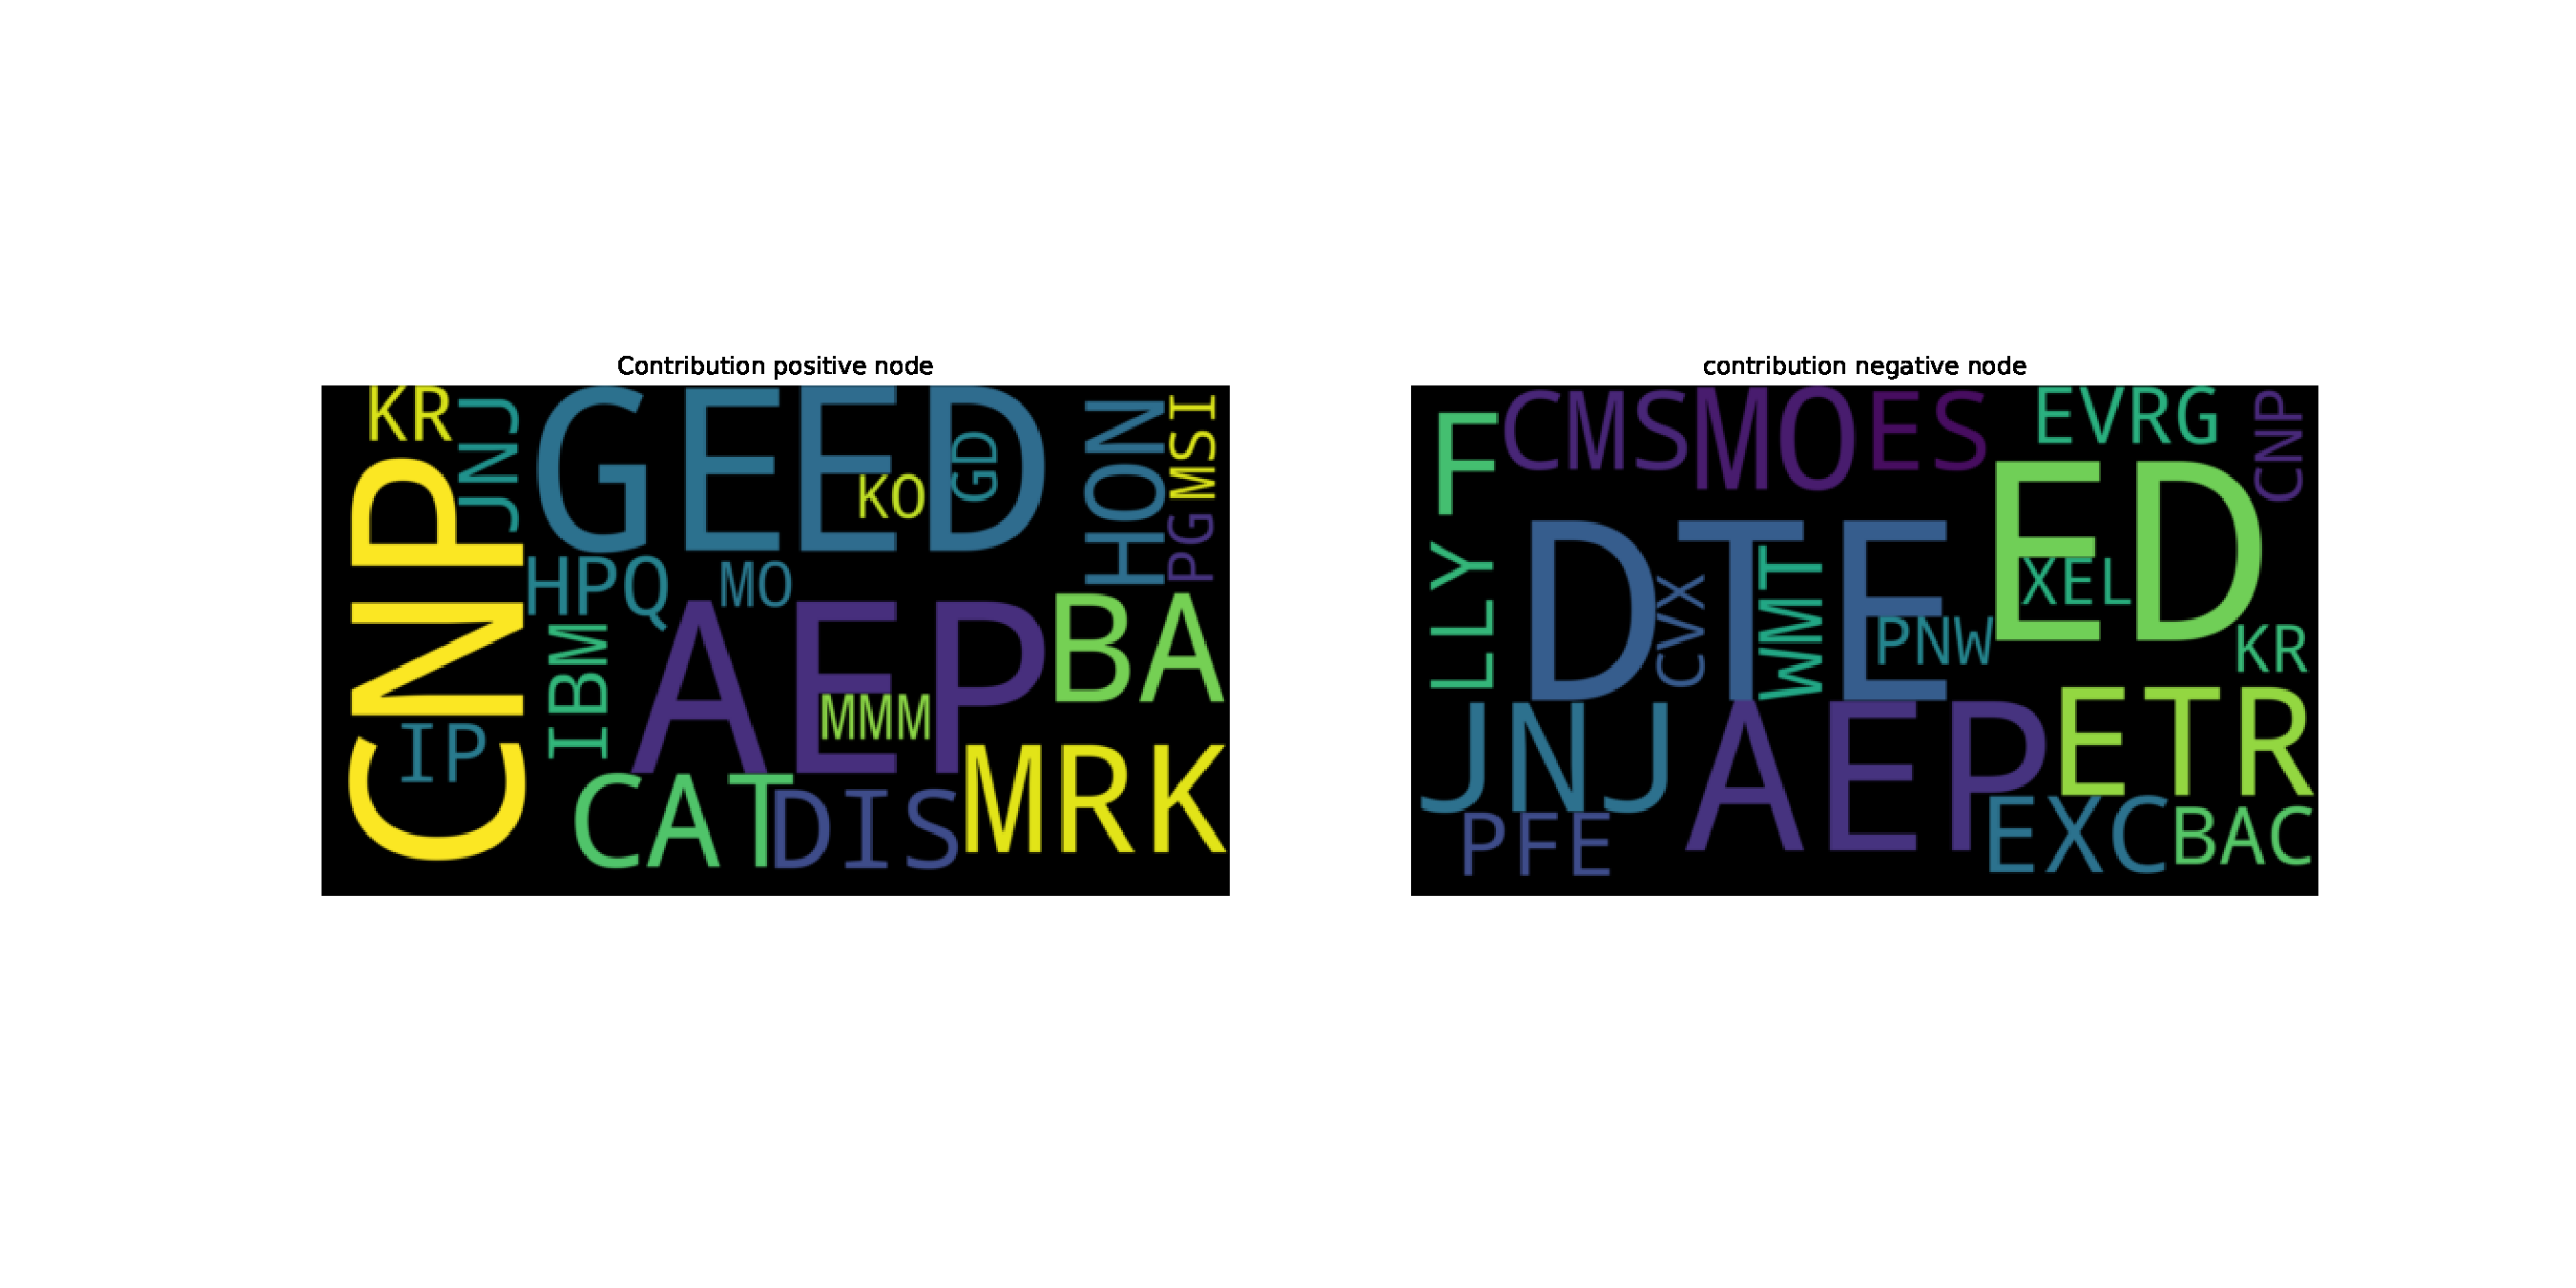
\includegraphics[width=\linewidth]{plot/wordcloud_contribution.pdf}
	\caption{Wordcloud Contribution}
\end{figure}
\begin{figure}[H]
	\centering
	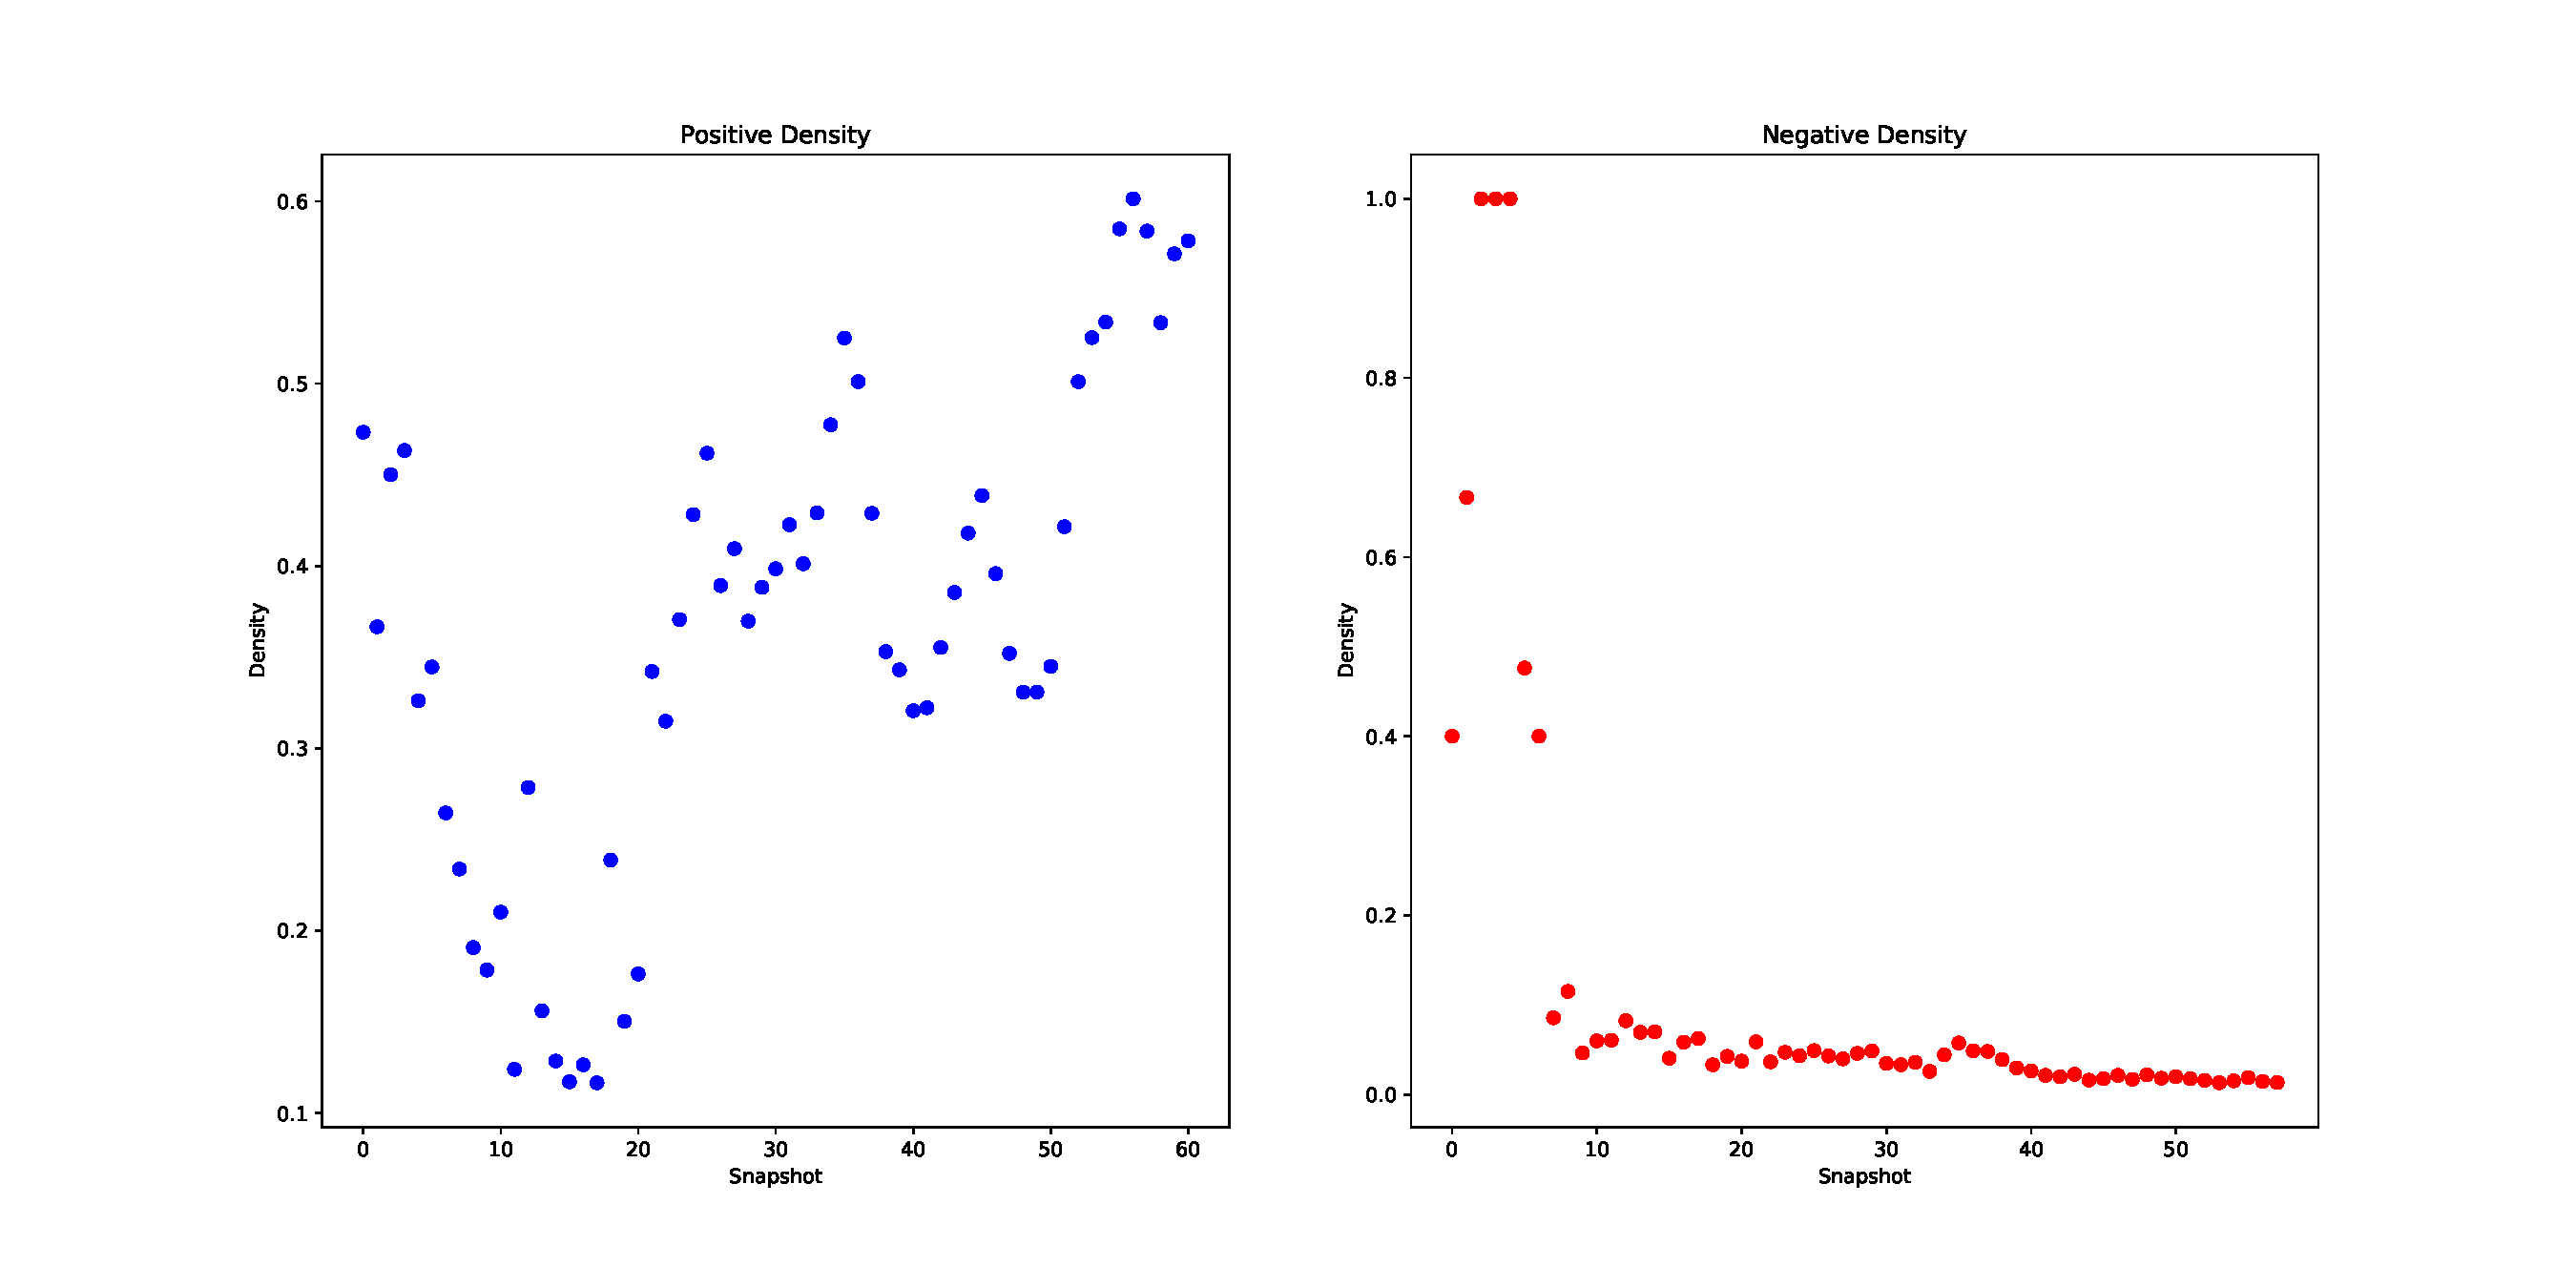
\includegraphics[width=\linewidth]{plot/density_dynamic.pdf}
	\caption{Density over snapshot}
\end{figure}
\section{Task 2: Static Community Discovery}
In this section we focus on the detection of static community discovery. To do so, we will study the overall graph,  \texttt{pos\_graph\_tot.gpickle}.
We have applied four different static community discovery algorithms (Leiden, Girvan-Newman, Newman’s leading eigenvector, Label propagation) to understand how various types of methods interact with our financial network. We begin by analysing the two cases in which the result is negative, no relevant partitions is returned : Girvan-Newmann and Label propagation. In the first case, it appears that, although the dendrogram is interrupted at various levels (in particular up to 30), there is only one large central cluster with many communities of very small size (< 3 nodes). The explanation is to be found in the high density of the network and its relative compactness due to the strong global trend component that characterises stock markets: subtracting even 
a significant fraction of the links leads to separating nothing but few shares.
It is an example of how the two heuristic ideas of community partitioning (density vs bridges) do not always lead to similar results, particularly for very dense graphs in which the identification of bridges has little meaning.
\begin{figure}[h]
	\centering
	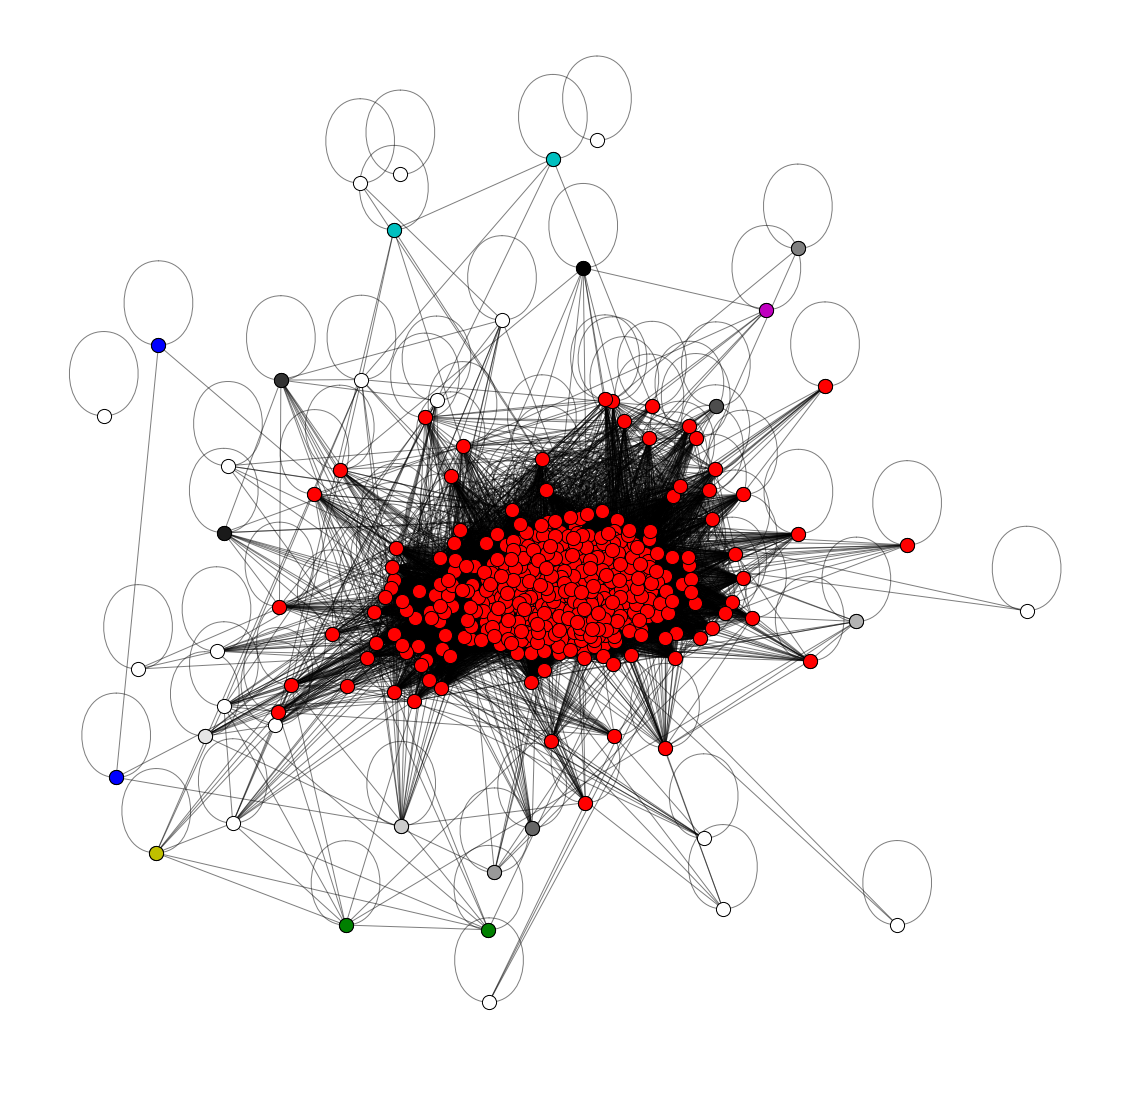
\includegraphics[width=\linewidth]{CD_GN.png}
	\caption{CD with GN algorithm at level 30, graphical representation}
\end{figure}

The label propagation algorithm, on the other hand, leads to an opposite result, albeit for the same reasons: since this is based on a bottom-up approach instead of a top-down one, the high density and compactness of the network does not allow for the aggregation of communities: each node remains separate.

\begin{figure}[h]
	\centering
	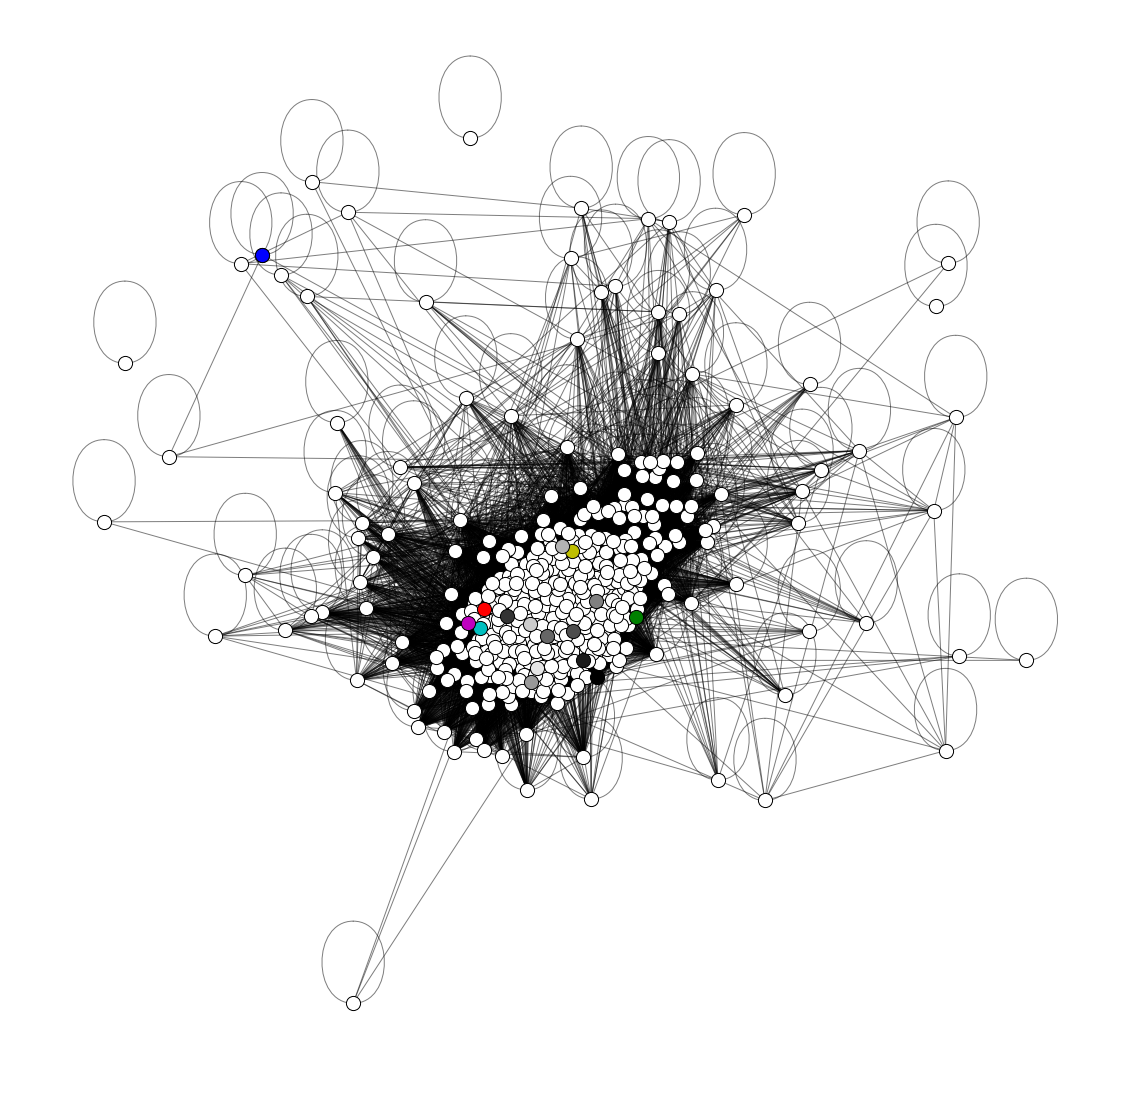
\includegraphics[width=\linewidth]{CD_lp.png}
	\caption{CD with LP algorithm, graphical representation. White nodes are not a }
\end{figure}

The two remaining algorithms, Leiden and Newman's leading eigenvector, lead to results that are a little more interesting: both identify two large clusters, which are, moreover, mutually consistent as we shall see later on, which is partly to be expected given that both are linked to the use of modularity as a value to be maximised. The coincidence between the two is however of interest given that they present two quite different methods: Leiden's algorithm has a bottom-up approach with a standard greedy procedure, while Newman’s leading eigenvector algorithm is top-down, algebraic one. 
With these two methods, based on the maximisation of an objective function, one does not run into the difficulties seen above due to the compactness of the network.

\begin{figure}[H]
	\centering
	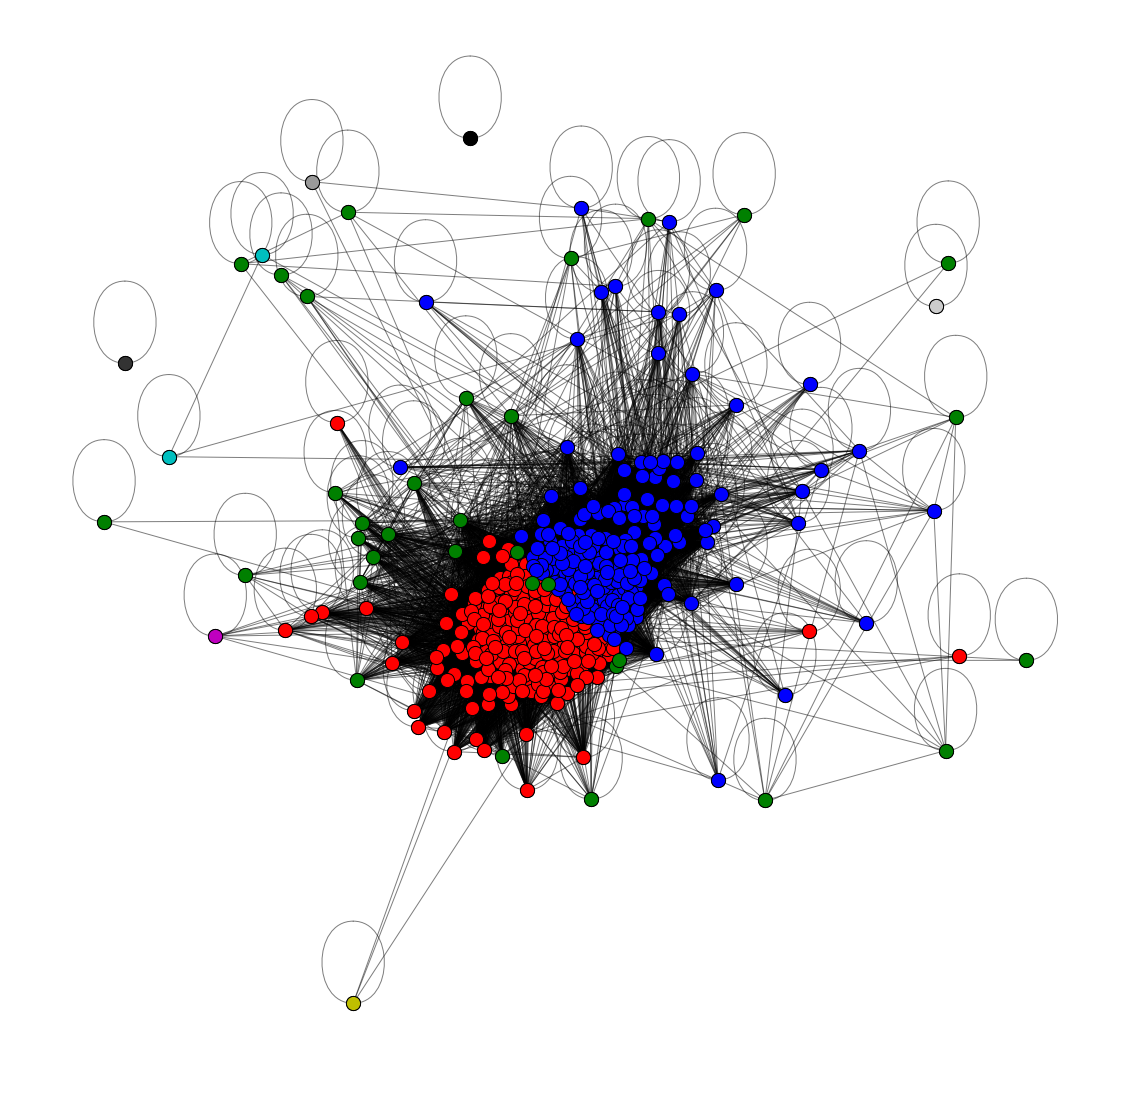
\includegraphics[width=\linewidth]{CD_lei.png}
	\caption{CD with Leiden algorithm, graphical representation.}
\end{figure}

\begin{figure}[H]
	\centering
	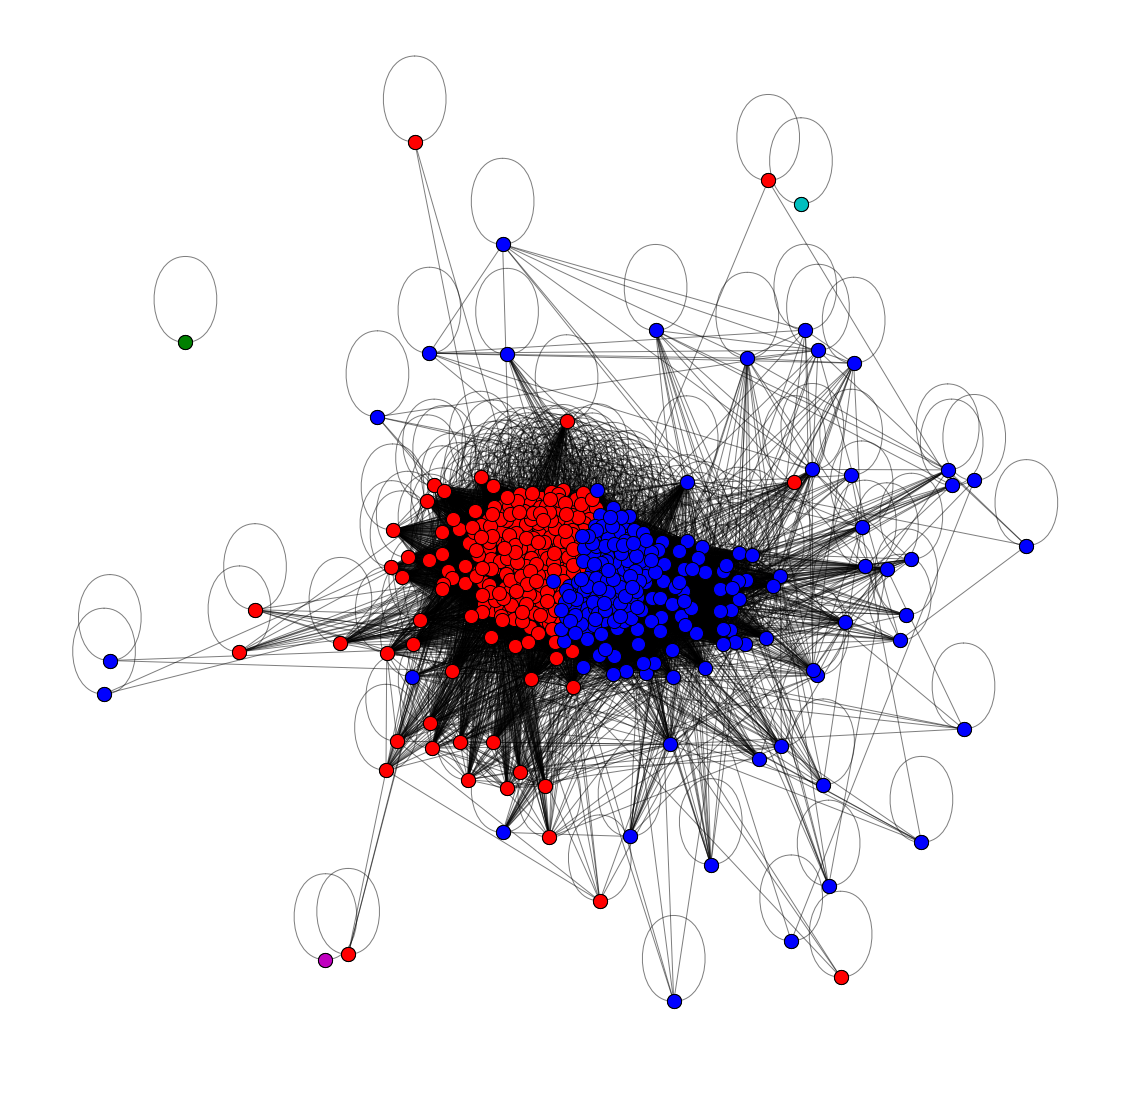
\includegraphics[width=\linewidth]{CD_Eig.png}
	\caption{CD with Newman's leading eigenvector algorithm, graphical representation.}
\end{figure}

We employ both internal and external measures as evaluation tools. Of the former type, we are interested in modularity and conductance. Of the second, we will compare both the various partitions with each other and with the ground truth offered to us by the sectoral classification of listed companies.
The following table summarises the results of the two statistics:

\begin{center}
\begin{tabular}{|c|c|c|}
\hline
Algorithm & Modularity & Conductance\\
\hline
Leiden & 0.0969 & 0.4445\\
\hline
Leading eigenvector & 0.0962  & 0.4071 \\
\hline
Girvan-Newman & 0.0016 & 0.6586 \\
\hline
Label propagation & 0.0052  & 0.9677 \\
\hline
\end{tabular}
\end{center}

Even the two algorithms based on modularity do not perform satisfactorily with this statistic, among other things producing a result of similar quality.
This is probably again attributable to the great compactness of the graph.
The other proposed internal evaluation measure also identifies Louvain and Leading eigenvector as higher quality partitions.
Finally, from the following graph (\ref{fig:26}
}) we can get an idea of the internal density for each of the various cummunities identified through the various algorithms as a function of their respective size (number of nodes).

\begin{figure}[H]
	\centering
	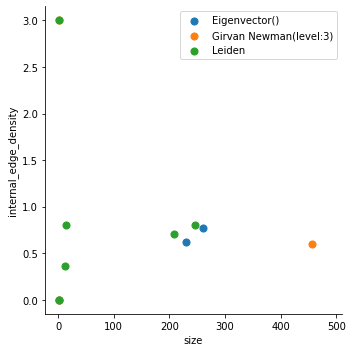
\includegraphics[width=\linewidth]{int_den_graph.png}
	\caption{Internal density vs size of community. Label propagation not represented}
	\label{fig:26}
\end{figure}

Again, 
In order to compare the various partitions obtained, we employ adjusted mutual information, which is actually more useful in quantifying how correct is the idea that the Leiden algorithm and Newman's leading eigenvector algorithm actually provide similar responses. Indeed, only for this pair of partitions does the index in question take on a significant value, and in particular it is worth around 0.73. The similarity matrix summarises these comparisons.


\begin{figure}[H]
	\centering
	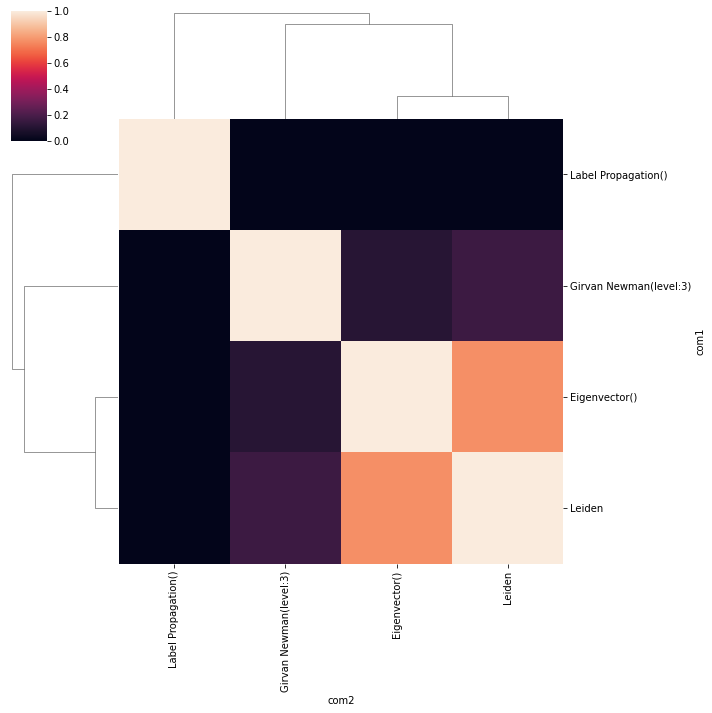
\includegraphics[width=\linewidth]{simm_mat.png}
	\caption{Similarity matrix with adjusted mutual information. Clearly only the communities detected with Leiden and Newman's leading eigenvector algorithm are coherent}
\end{figure}

The same index was also used for the ground truth comparison: using the GICS (Global Industry Classification Standard, the industrial taxonomy eployed by Standard&Poor's, the corporation that builds the SP500 index) a partition of 11 communities was constructed based precisely on the sectoral affiliation of each company. Given the great disparity in number and relative size, intuition suggests that agreement will be rather poor.
In fact, ignoring the two algorithms that produced no useful results, Leiden and Newman's leading eigenvector algorithms are also rated 0.0719 and 0.0591 respectively.
The idea behind this comparison is that companies belonging to the same sector are subject to similar exogenous shocks, thus experiencing greater correlation in their respective share prices and thus being 'candidates' for clusters. 
The failure of this hypothesis may be due to several factors: for instance, it may be that the influence of sectoral shocks is limited when compared to shocks of another nature, such as the general business cycle or geographical shocks. Alternatively, it could be the choice of algorithms employed that are not appropriate. Or again, even if the sectoral component is significant in determining correlations between stock price movements, the chosen threshold of 0.7 is not sufficient to filter out larger scale components ( again, the business cycle, even of distinct geographic areas). The high density of the network is a clue, leaning in this case towards the third, or possibly the first, hypothesis.


\section{Task 3: Dynamic Community Discovery}
In this section, we will show, over a limited time interval (2010-2014), the evolution of communities in our financial network and the tools used to explore this aspect of the topic under investigation. 
We employed two different methods to reconstruct the history of communities: instant optimal and tiles. To these, we coupled the same algorithms used in the previous section to identify communities at a certain snapshot: as it previously turned out, the use of the label propagation algorithm has not proved effective for studying the behaviour of financial networks, so in this section we will not present the results for this community detection criterion, which in any case are inconclusive, as no community of relevant size has ever been circumscribed.
Before presenting these results, we report the values of the temporal stability assessments of the identified communities, which are independent of the way the dynamic is reconstructed, obtained using the Normalized F1 score.

\begin{center}
\begin{tabular}{|c|c|c|c|c|}
\hline
Alg. \ year & 10/11 & 11/12 & 12/13 & 13/14 \\
\hline
Leiden & 0.051 & 0.116 & 0.068 & 0.179\\
\hline
Lead. eigen. & 0.200  & 0.059 & 0.055 & 0.062 \\
\hline
GN & 0.053 & 0.093 & 0.047 & 0.037 \\
\hline
\end{tabular}
\end{center}

Let us now see the outcome of the instant optimal algorithm in conjunction with the GN algorithm: the graphs in the figure are polytrees that have as nodes the communities at a given time instant and as oriented arcs the identifications from one year to the next between the communities. With the algorithm, which has as input the jaccard index ($J(A, B) = \frac{|A \cap B}{|A \cup B|} $, where $A$ and $B$ are sets), merges and spilts of communities are determined. 
As Figure 33 makes clear, once the smaller communities have been eliminated, the evolution is rather limited: only one large community persists over the five years considered. Studying its size trend, we find that there is a tendency for its size to increase (from 439 to 464), due to the nodes being added to the financial network as they go along.

\begin{figure}[H]
	\centering
	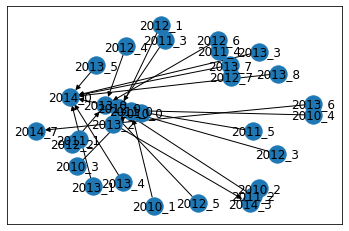
\includegraphics[width=\linewidth]{polyt GN full.png}
	\caption{Polytree of dynamic community discovery with instant optimal algorithm, applied to communities discovered with GN algorithm.}
\end{figure}

\begin{figure}[H]
	\centering
	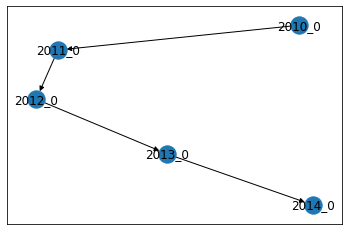
\includegraphics[width=\linewidth]{polyt GN removed.png}
	\caption{Polytree of dynamic community discovery with instant optimal algorithm, applied to communities discovered with GN algorithm. Small ( < 5 nodes) communities have been removed}
\end{figure}

Turning now to the results obtained with the GN algorithm, the story told by the 'cleaned-up' polytree of the smaller communities is richer: initially there are only two relevant communities, both stable with just over 200 nodes, in 2012 a third community with 100 nodes appears, while the larger of the two already existing communities loses about 80 members, only to reabsorb in 2014 'the newest arrival'.

\begin{figure}[H]
	\centering
	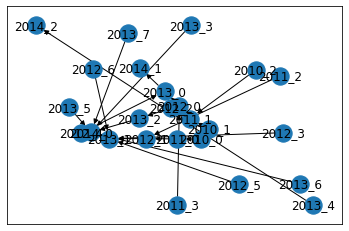
\includegraphics[width=\linewidth]{polyt eig full.png}
	\caption{Polytree of dynamic community discovery with instant optimal algorithm, applied to communities discovered with Newman’s leading eigenvector method.}
\end{figure}

\begin{figure}[H]
	\centering
	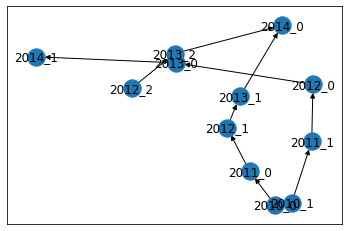
\includegraphics[width=\linewidth]{polyt eig removed.png}
	\caption{Polytree of dynamic community discovery with instant optimal algorithm, applied to communities discovered with Newman’s leading eigenvector method. Small ( < 5 nodes) communities have been removed}
\end{figure}

The last algorithm, Leiden, is undoubtedly the one that gives us the most complex case: in 2010 there are four different communities of significant size (171, 147, 89, 33 respectively). After some variation in size in 2011, in 2012 there is the merger of the largest with the smallest, while the others experience fluctuations in size.

\begin{figure}[H]
	\centering
	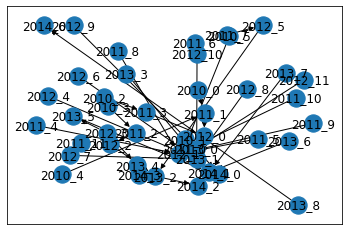
\includegraphics[width=\linewidth]{polyt lei full.png}
	\caption{Polytree of dynamic community discovery with instant optimal algorithm, applied to communities discovered with Leiden algorithm.}
\end{figure}

\begin{figure}[H]
	\centering
	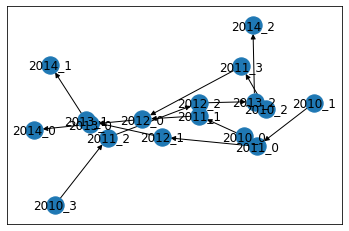
\includegraphics[width=\linewidth]{polyt lei removed.png}
	\caption{Polytree of dynamic community discovery with instant optimal algorithm, applied to communities discovered with Leiden algorithm. Small ( < 5 nodes) communities have been removed.}
\end{figure}	
	
The other method used to reconstruct the temporal evolution of communities places less emphasis on those identified in individual frames and prefers to build them incrementally as the network evolves.
Because of this characteristic, the brevity of the analysed interval and the lack of stability and poor definition of the communities (e.g. we have just seen that the three previous algorithms return three different narratives), the results are unenlightening.
\newline
Going to interrogate the first polytree of this series of three, the one where communities are produced with GN algorithm: we observe that there are no communities from the last two snapshots. Beyond this, we observe two functions, the first of three entities and the second of two.
	
\begin{figure}[H]
	\centering
	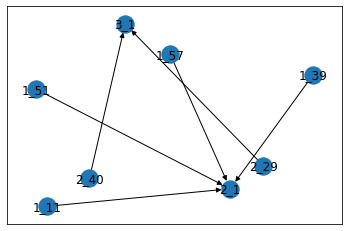
\includegraphics[width=\linewidth]{polyt GN tiles.png}
	\caption{Polytree of dynamic community discovery with tiles method, applied to communities discovered with GN. Small ( < 5 nodes) communities have been removed.}
\end{figure}

As in the previous one, in this second polytree obtained with Newman's leading eigenvector method, no communities were identified in the last two snapshots. Mergers are also recorded here.

\begin{figure}[H]
	\centering
	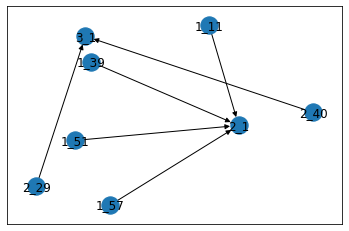
\includegraphics[width=\linewidth]{polyt eig tiles.png}
	\caption{Polytree of dynamic community discovery with tiles method, applied to communities discovered with Newman’s leading eigenvector method. Small ( < 5 nodes) communities have been removed.}
\end{figure}

The last polytree in the series, where the communities were identified with the Leiden algorithm, has the same characteristics as the others.

\begin{figure}[H]
	\centering
	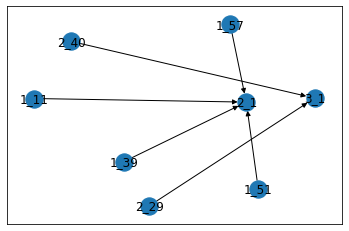
\includegraphics[width=\linewidth]{polyt lei tiles.png}
	\caption{Polytree of dynamic community discovery with tiles method, applied to communities discovered with Leiden algorithm. Small ( < 5 nodes) communities have been removed.}
\end{figure}

\section{Task 4: Stock market crush and networks}

In this section, we try to answer the question that prompted the project: do graph theory tools have anything to say about times of major upheavals in the financial markets, such as mounting speculative bubbles and subsequent crashes, or even during intense shocks such as the collapse due to the Coronavirus pandemic? To do so, let us study how the main network-defined statistics behave during the various phases that stock markets experience: speculative boom and bust ('07-'10), March-April 2020 (pandemic shock) and a standard period (1985). In this section, correlations are calculated over a 40-day time interval, with rolling windows of 20 days.
A further difference from the previous sections, here we study a weighted graph: each arc has assigned a value called distance calculated as follows: $ d = \sqrt{2(\rho-1)}$. Note that the higher the distance, the less strong the link between two stocks, as they are less correlated.
The first tool used is the heat map: scrolling from left to right we encounter: in a normal period there are no sectors that stand out above the others. In the second grid, we can see that two sectors, nominally energy and IT sector, show a high level of clustering: this is an indicator of a possible bubble: a certain production sector is considered promising per se, without distinguishing between individual companies. When the moment of collapse arrives (third heat map), the previous hypothesis is verified, in particular the sectors whose share prices had been driven up by enthusiasm and not by rational evaluations are discovered.
The collapse related to the pandemic shock resembles the crash period of the previous situation: after all, it was an event that negatively impacted most sectors.
\begin{figure}[H]
	\centering
	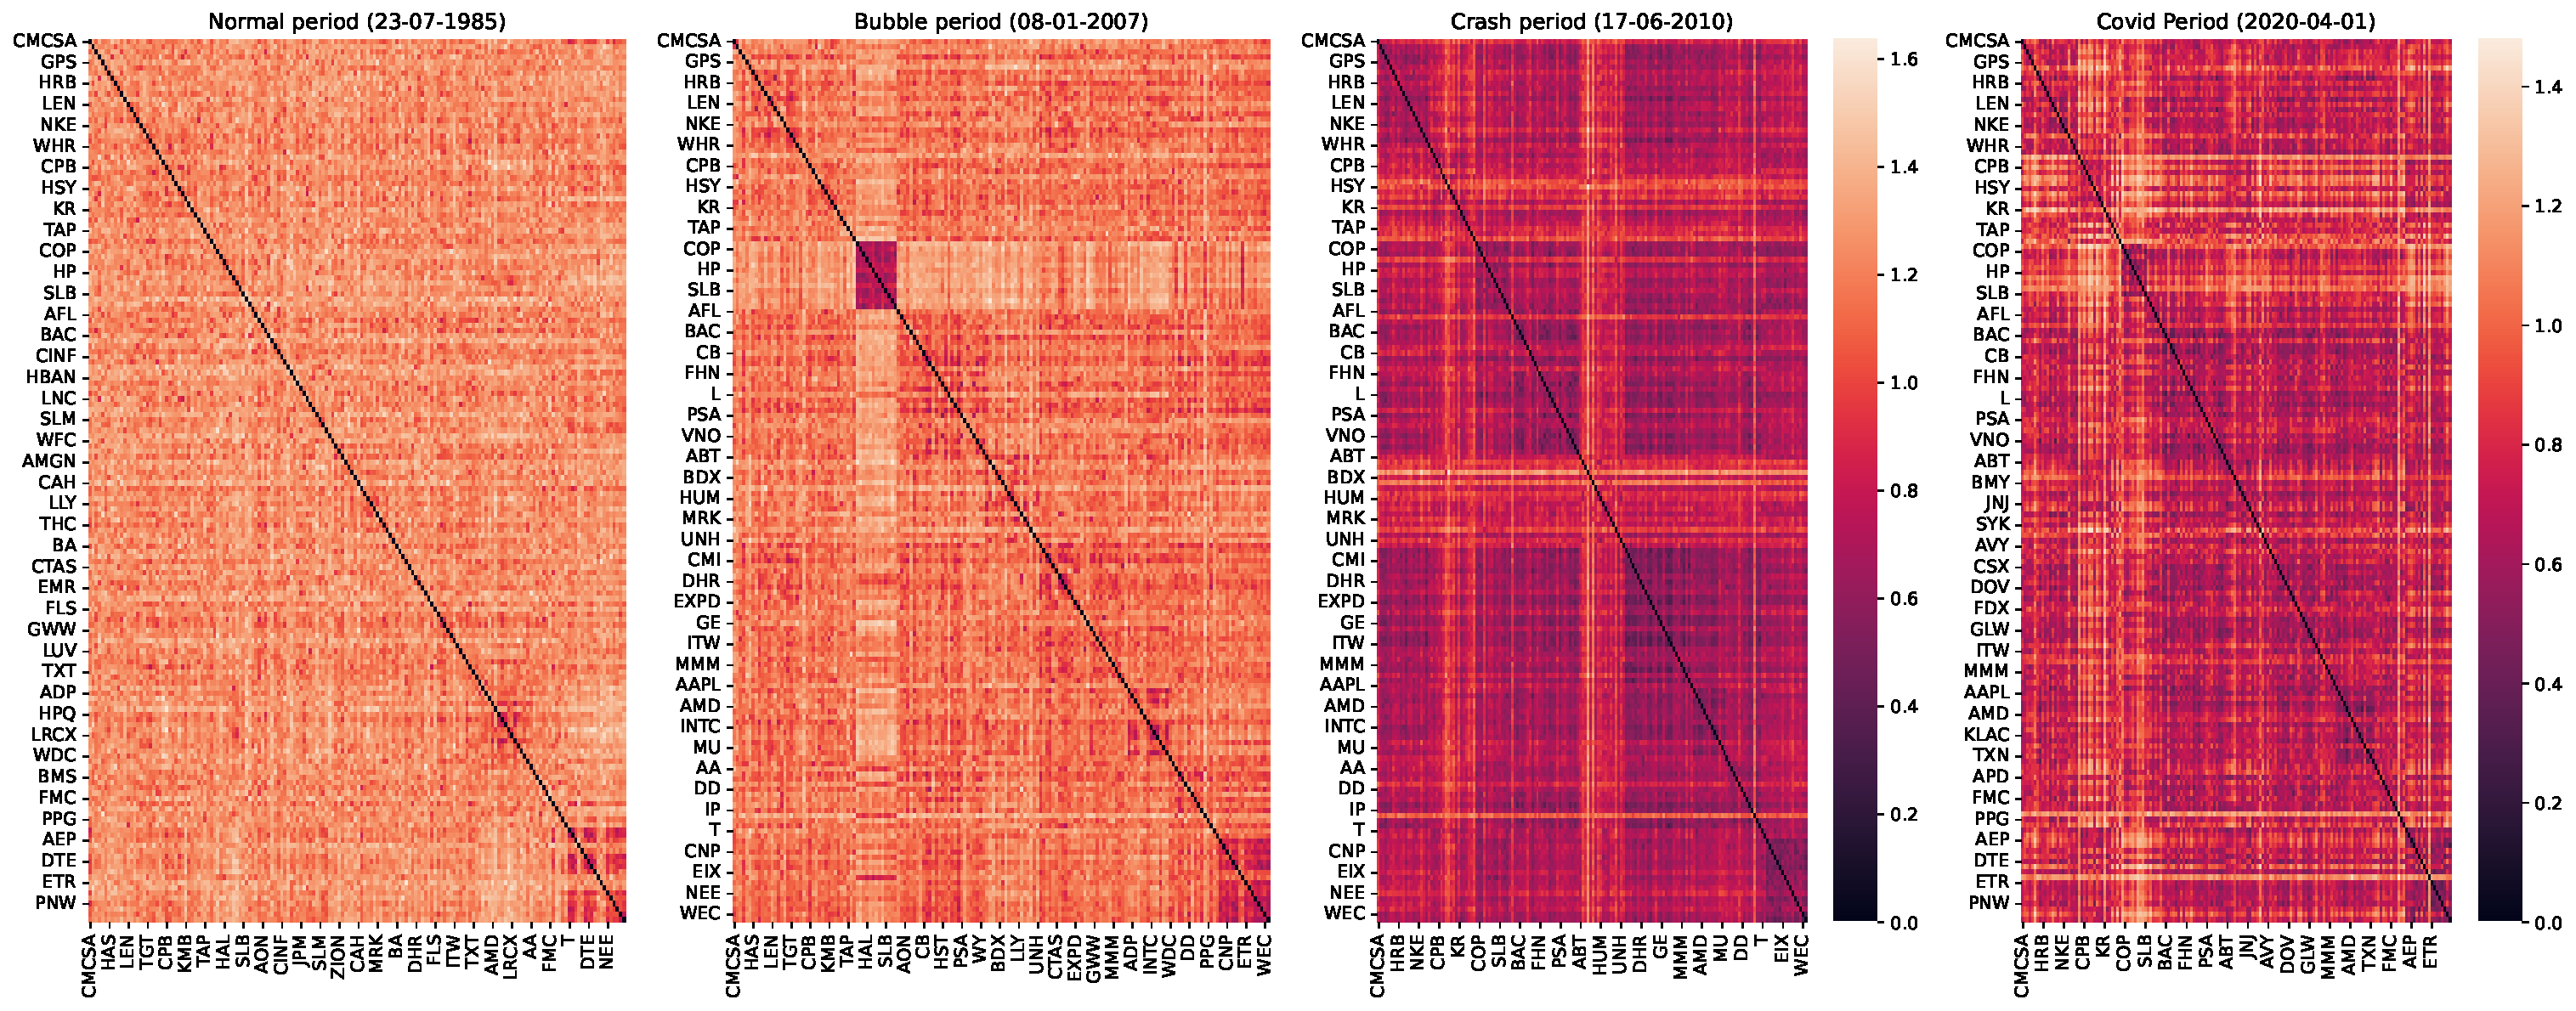
\includegraphics[width=\linewidth]{heatmap a confronto.pdf}
	\caption{Heatmap at various market periods}
\end{figure}
Similar conclusions are also suggested to us by another useful tool for investigating the topology of the fianncial network and how it evolves: the Minimum spannig tree (MST) \cite{MST} offers a measure of how compact the stock market is overall. Again, in a period without turbulence, the financial network is sparse, unconnected and with few stocks speriementing interrelated price dynamics, so a few arcs suffice to make the minimum spanning tree. Something different happens progressively as one approaches a period of sharp declines in stock market indices: gradually more securities are aggregated from the central body of the minimum spanning tree and more edges are needed to realise it: stronger connections (i.e. higher correlation and lower distance) are gradually added, which make the various nodes even 'closer' and are thus selected by the greedy algorithm that produces the spanning tree.
Again, we observe how the collapse due to the pandemic has similar characteristics to the speculative event of 2008, although it was clearly not preceded by a bubble.
An advantageous feature of this tool is the clarity with which it provides an answer precisely because it only highlights the connections that are really necessary to illustrate how much the various prices of securities are moving together.\\
In order to have more information on the graph, it is possible to build the Planar Maximally Filtred Graph\cite{PMFG}, it has more information about the connection than MST.\\
\begin{figure}[H]
	\centering
	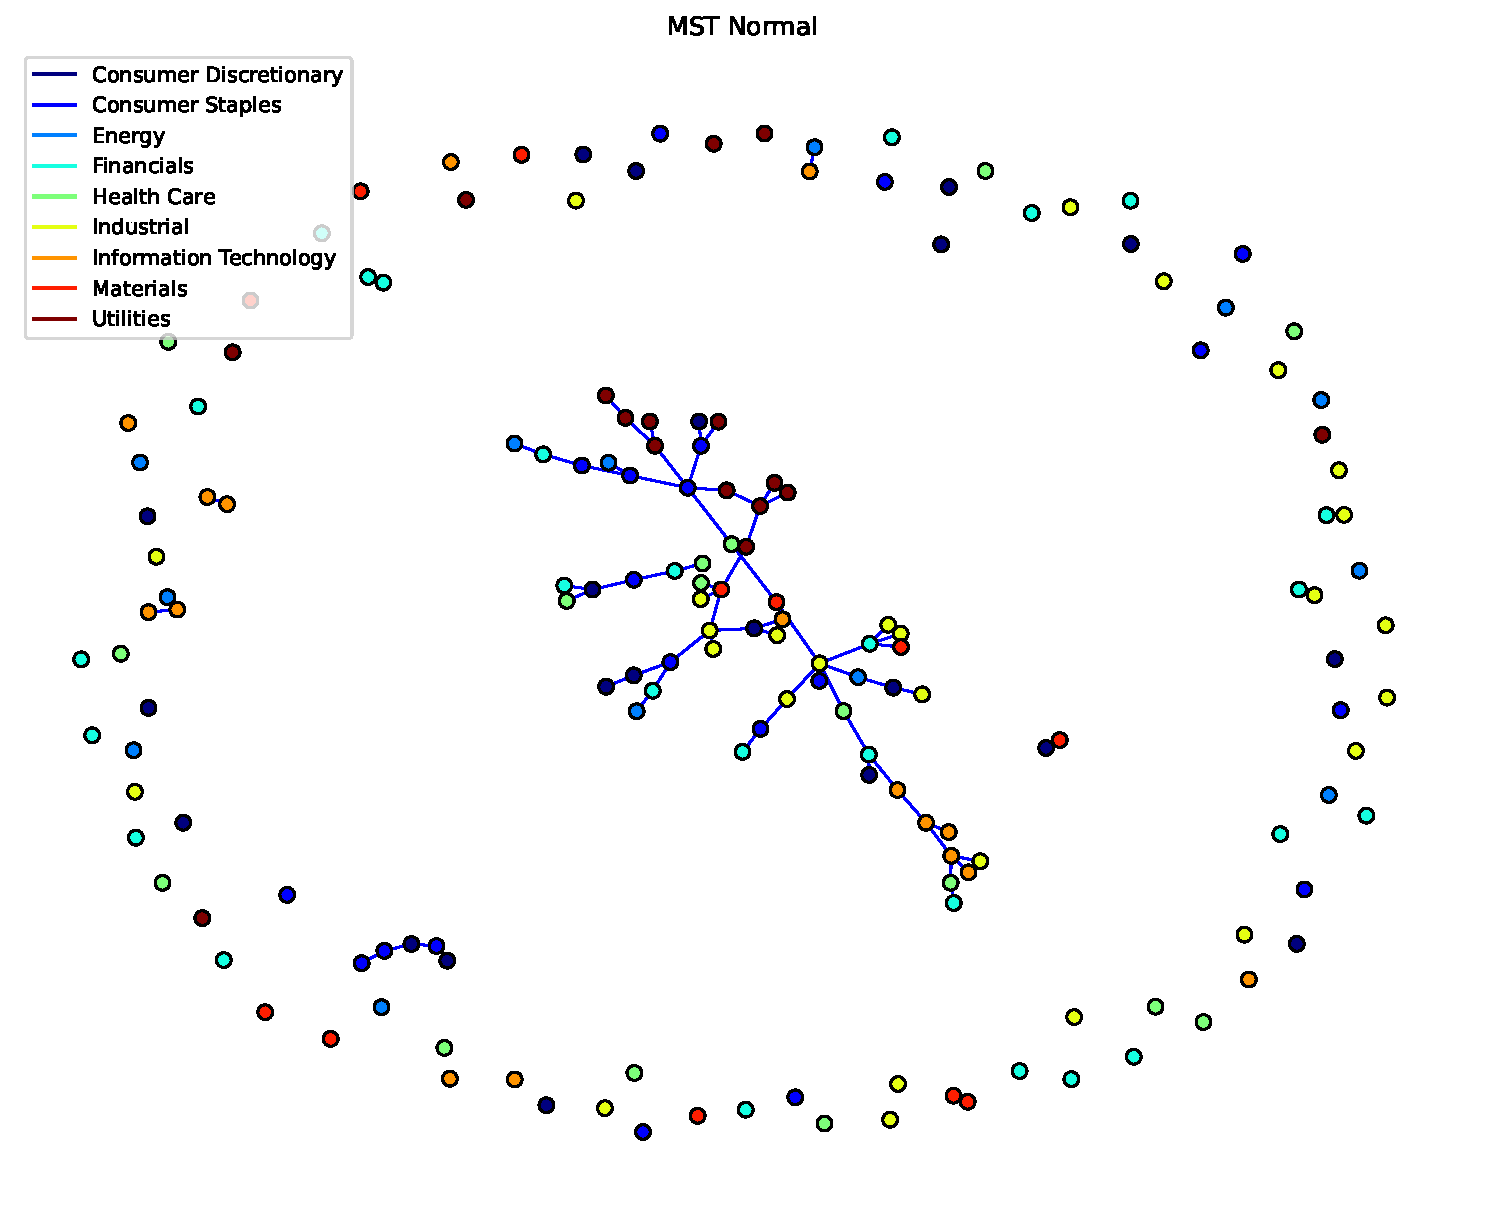
\includegraphics[width=\linewidth]{MST Normal.pdf}
	\caption{Minimum spanning tree in normal market period (1985)}
\end{figure}
\begin{figure}[H]
	\centering
	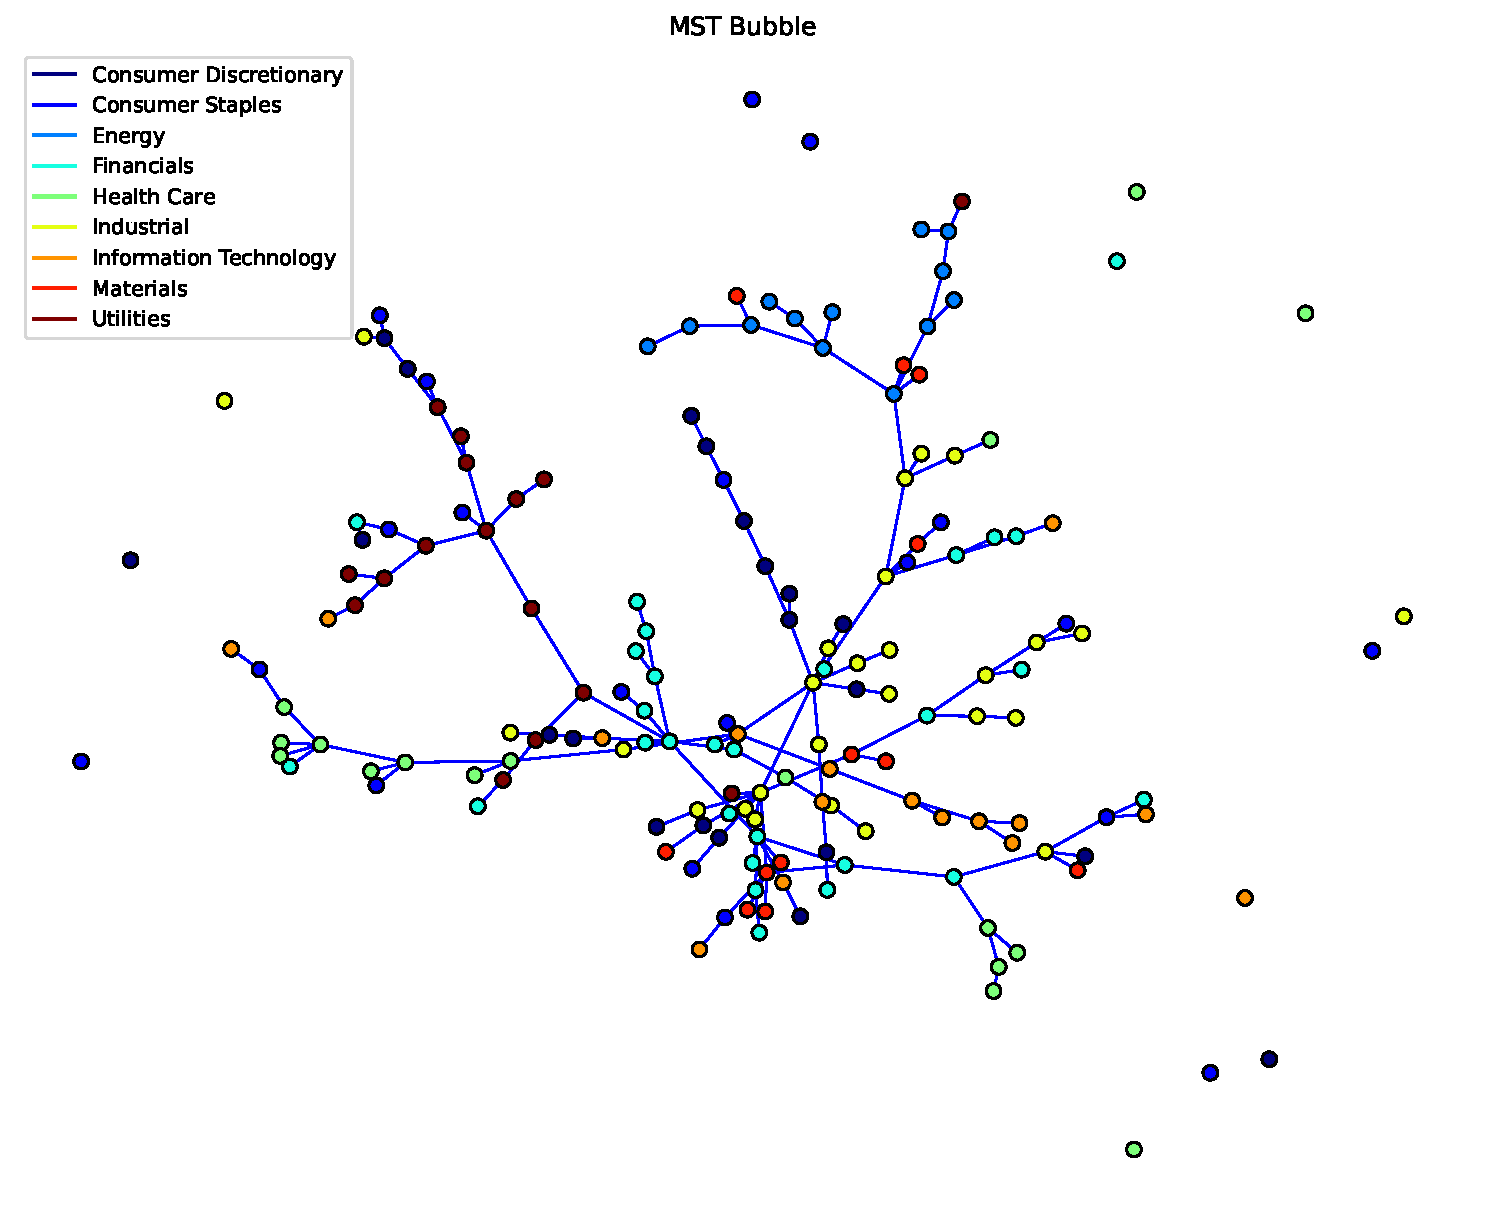
\includegraphics[width=\linewidth]{MST Bubble.pdf}
	\caption{Minimum spanning tree in bubble period (2007)}
\end{figure}
\begin{figure}[H]
	\centering
	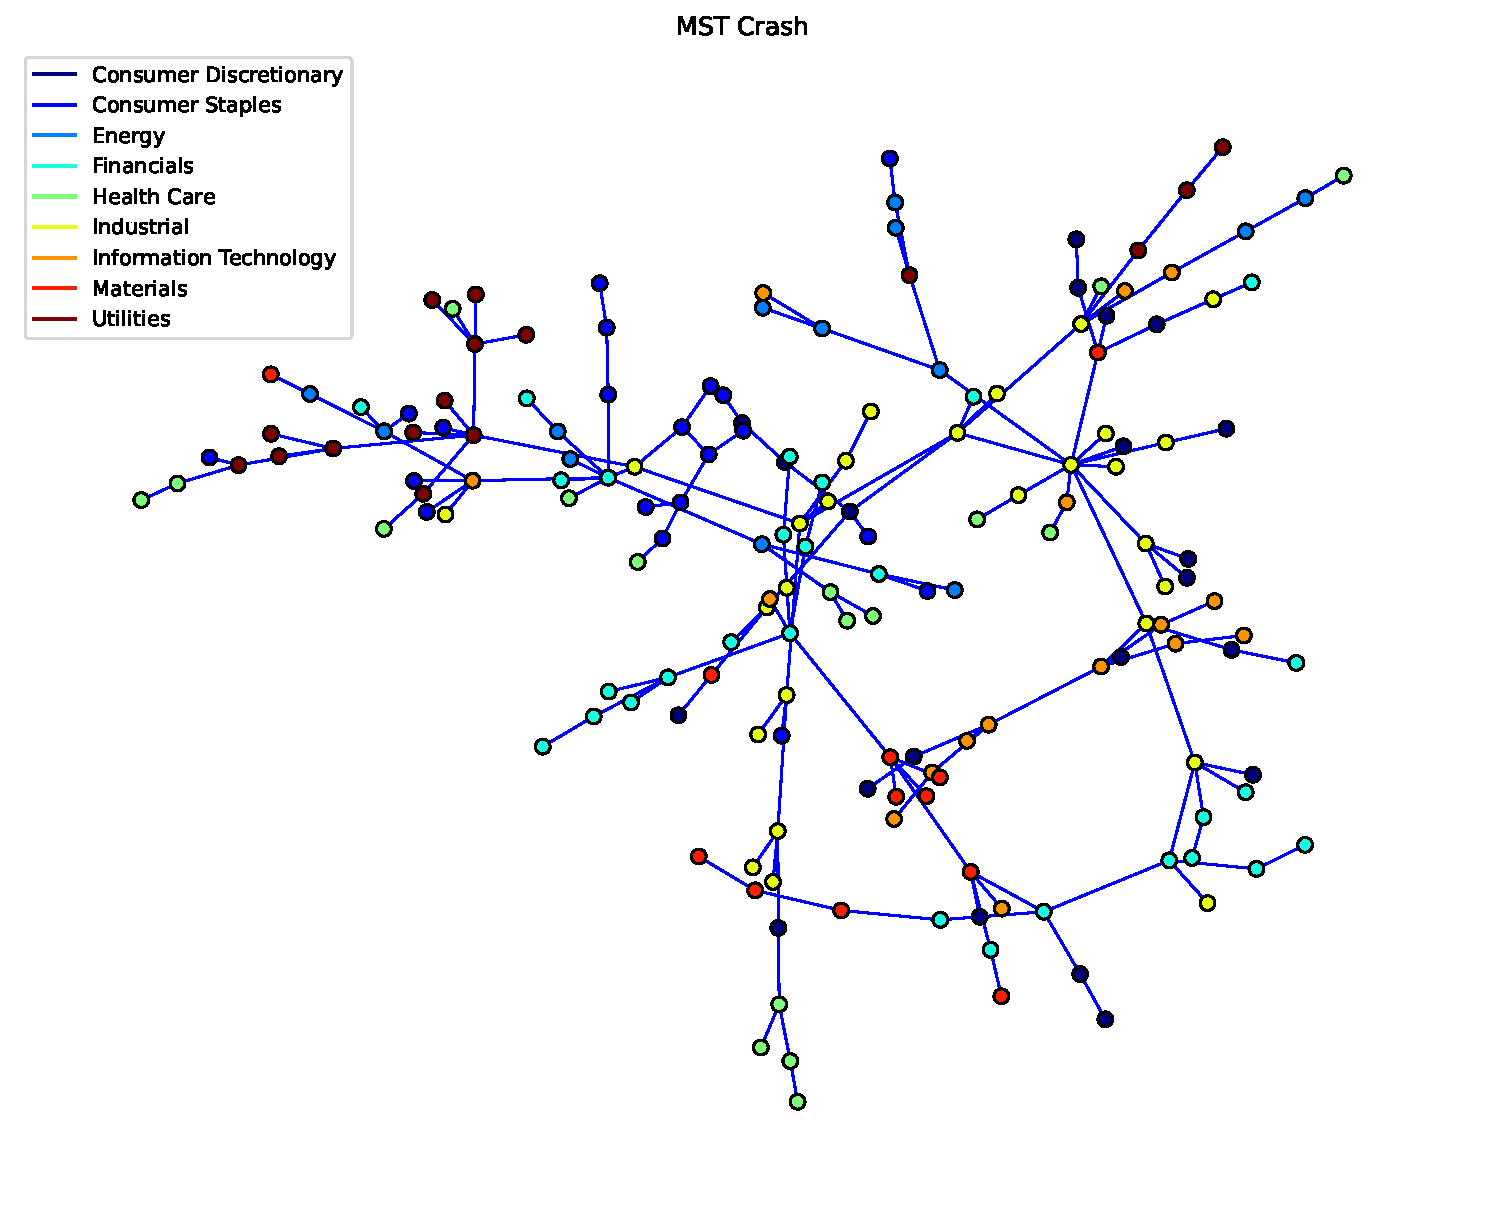
\includegraphics[width=\linewidth]{MST Crash.pdf}
	\caption{Minimum spanning tree in bust period (2010)}
\end{figure}
\begin{figure}[H]
	\centering
	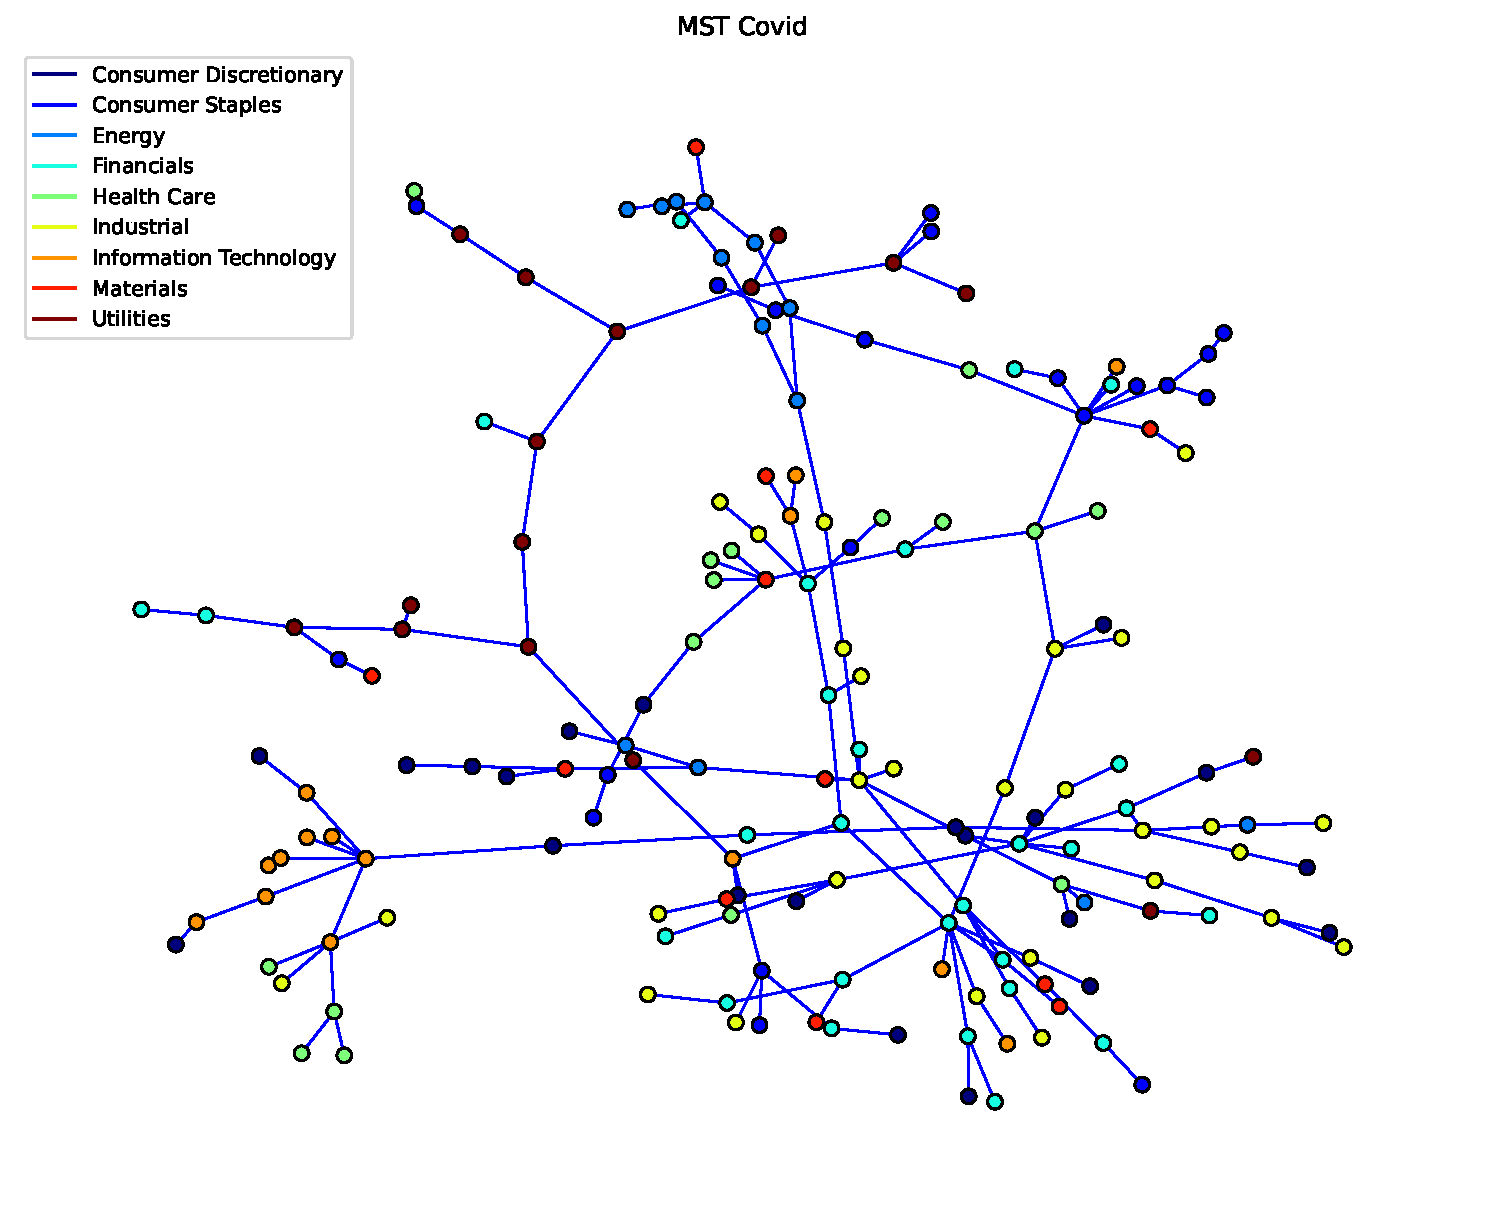
\includegraphics[width=\linewidth]{MST Covid.pdf}
	\caption{Minimum spanning tree in covid crisis period (2020)}
\end{figure}
The threshold network also suggests at a glance considerable qualitative differences between the normal state of the market and the more or less positive turmoil that invests it at other times: again, during the bubble's mounting, nodes begin to thicken as if preparing the bust's phase. Really a phase transition seemes to be at work: we observe an evolution from an highly dispersed network to a(n almost) fully connected one.\\
A further analysis on treshold network have been done to discover some graph's topological properties useful to characterized the three period:  Density and Global clustering are  first important values, an high value of density and Clustering Coefficient is symptom of crash period; the different shape of histogram of Local Clustering Coefficient gives us important information about Covid period: while during the Crash, almost all nodes have high values, for Covid the histogram have a left fat-tail shape, completely different from the previous ones.\\
Also betweenness centrality's during Covid period have a unique shape really different from previous one.\\
Assortative gives us another important parameter: in Crash and Covid period it is negative.
\begin{figure}[H]
	\centering
	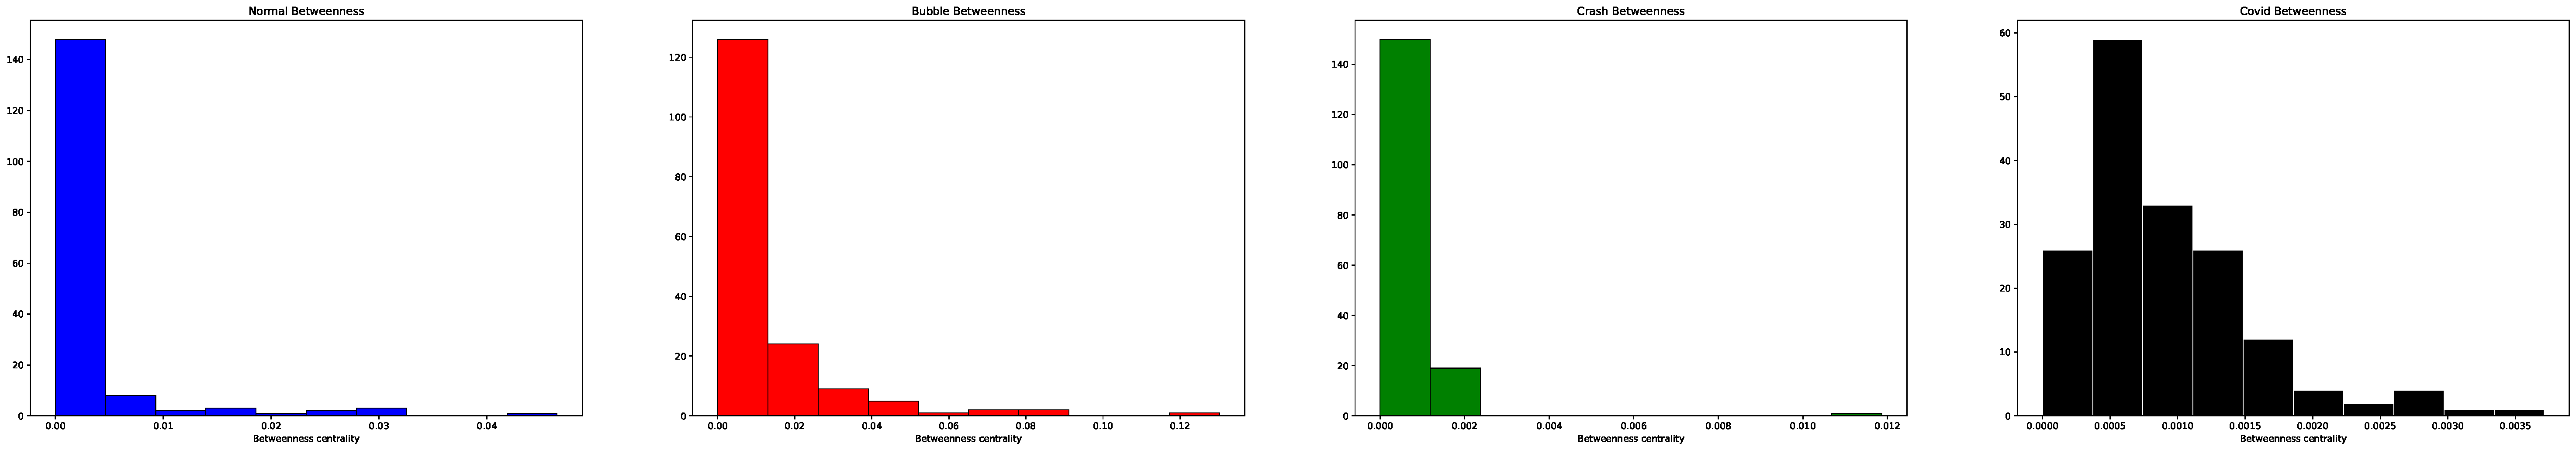
\includegraphics[width=\linewidth]{distribution_betweenness.pdf}
	\caption{Betweenness centrality Histogram}
\end{figure}
\begin{figure}[H]
	\centering
	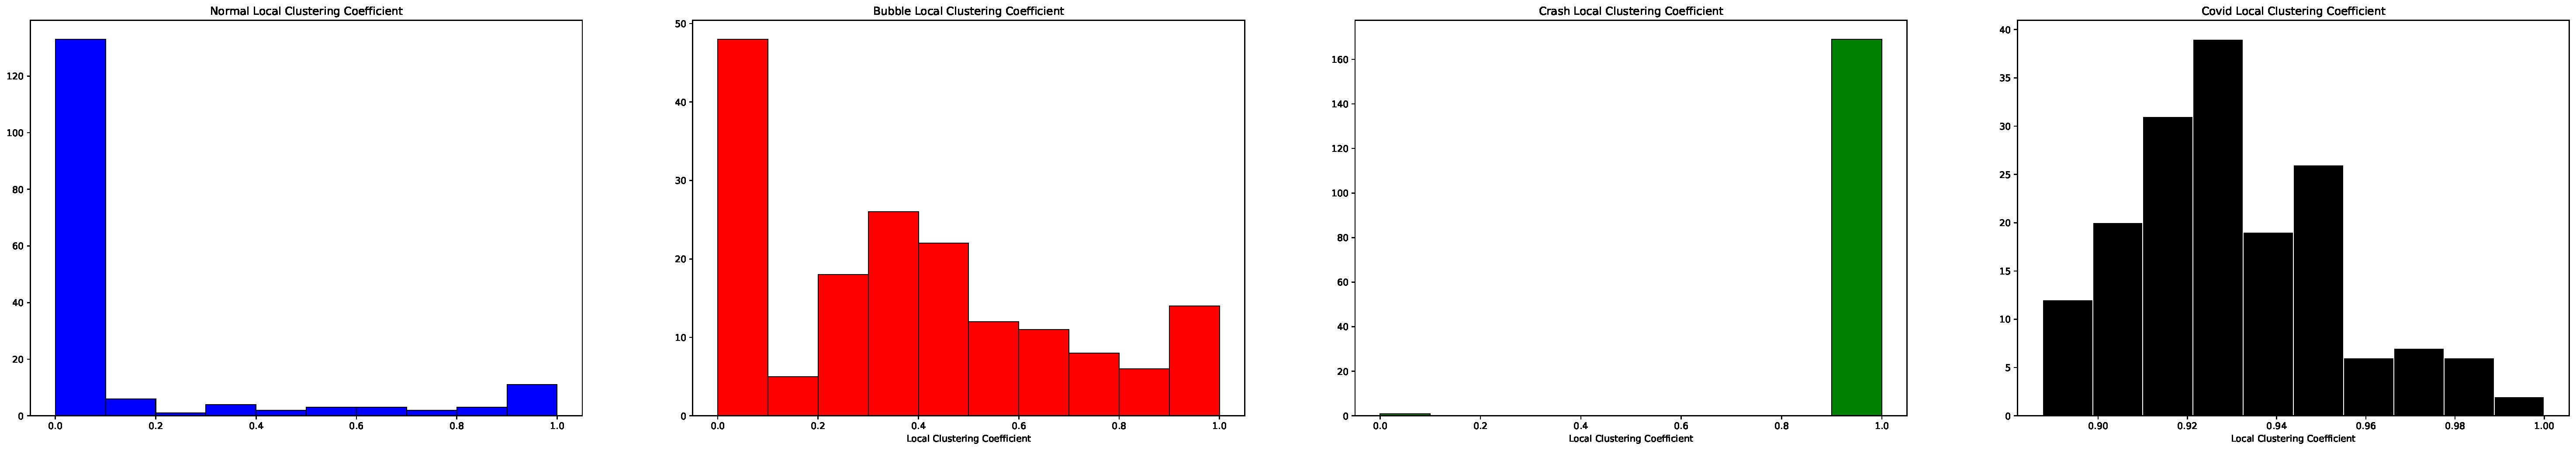
\includegraphics[width=\linewidth]{local_clustering_coefficient.pdf}
	\caption{Local Clustering Histogram}
\end{figure}
\begin{figure}[H]
	\centering
	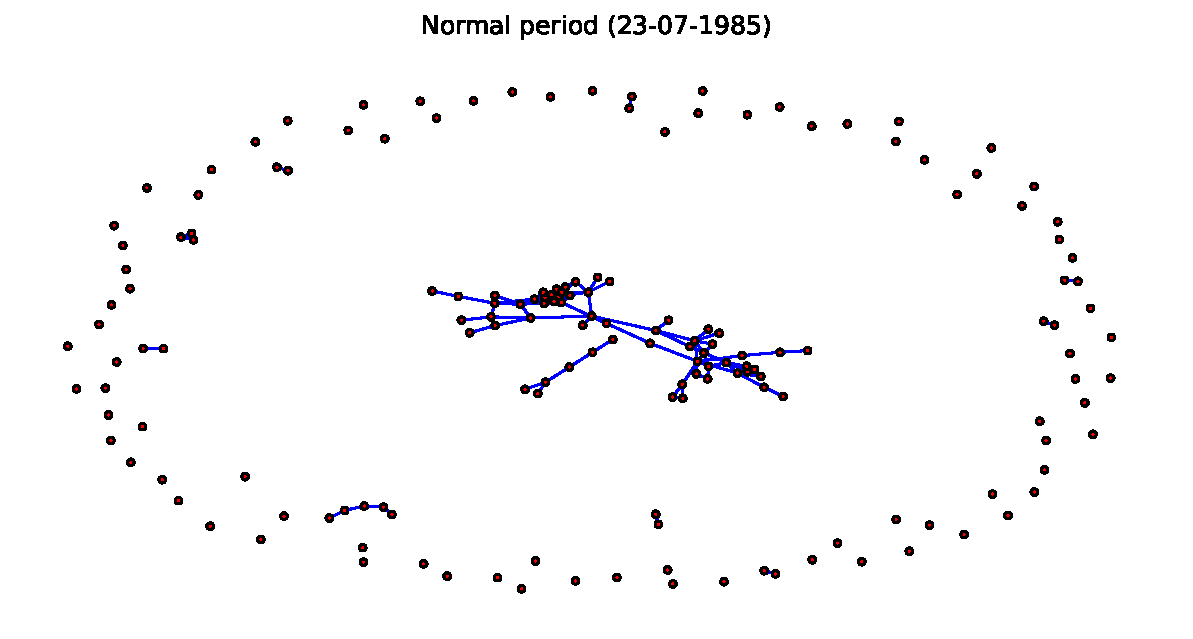
\includegraphics[width=\linewidth]{(1)tresh_normal.pdf}
	\caption{Threshold network with threshold d = 1 in normal market time (1985)}
\end{figure}
\begin{figure}[H]
	\centering
	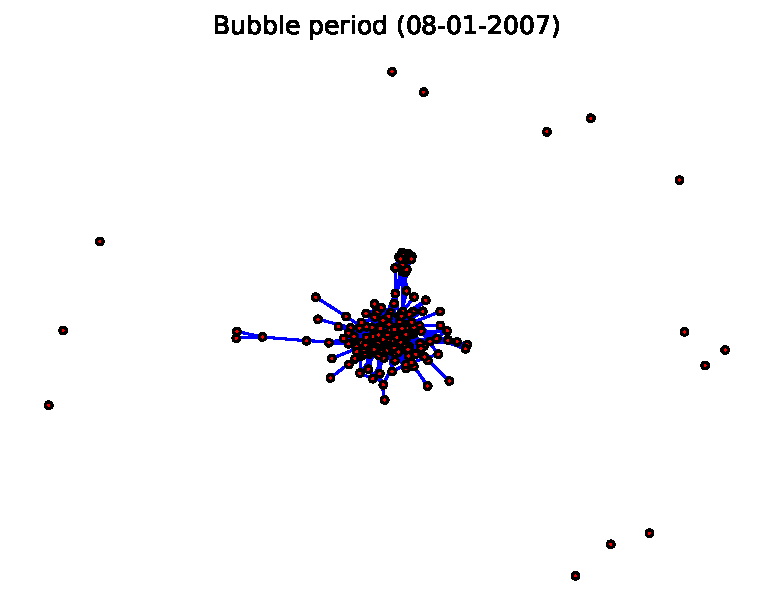
\includegraphics[width=\linewidth]{(2)tresh_bubble.pdf}
	\caption{Threshold network with threshold d = 1 in bubble period time (2007)}
\end{figure}
\begin{figure}[H]
	\centering
	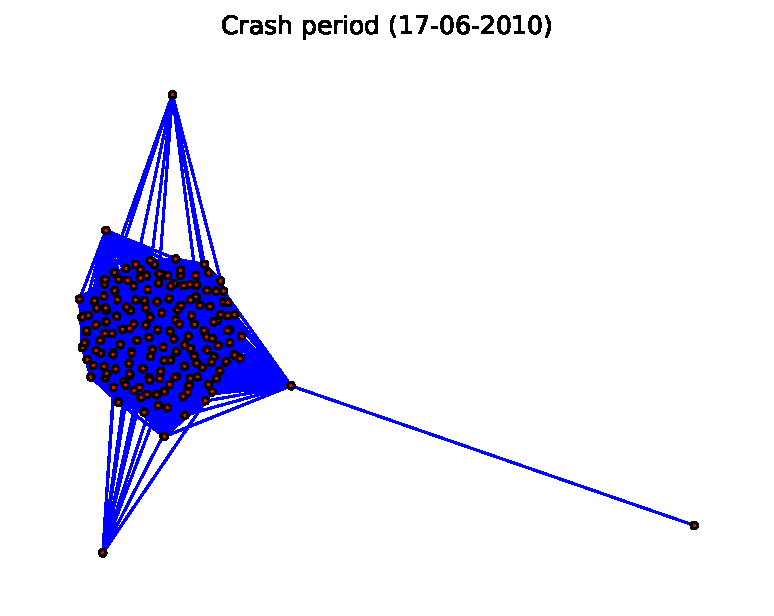
\includegraphics[width=\linewidth]{(3)tresh_crash.pdf}
	\caption{Threshold network with threshold d = 1 in crash time (2010)}
\end{figure}
\begin{figure}[H]
	\centering
	\includegraphics[width=\linewidth]{(4)tresh_covid.pdf}
	\caption{Threshold network with threshold d = 1 in covid crisis (2020)}
\end{figure}


\begin{figure}[H]
	\centering
	\includegraphics[width=\linewidth]{PMFG Normal.pdf}
	\caption{Planar maximally filtered graph of a normal market period (1985)}
\end{figure}
\begin{figure}[H]
	\centering
	\includegraphics[width=\linewidth]{PMFG Bubble.pdf}
	\caption{Planar maximally filtered graph of bubble period (2007)}
\end{figure}
\begin{figure}[H]
	\centering
	\includegraphics[width=\linewidth]{PMFG Crash.pdf}
	\caption{Planar maximally filtered graph of crash period (2010)}
\end{figure}
\begin{figure}[H]
	\centering
	\includegraphics[width=\linewidth]{PMFG Covid.pdf}
	\caption{Planar maximally filtered graph of covid crash (2020)}
\end{figure}

\begin{figure}[H]
	\centering
	\includegraphics[width=\linewidth]{eigen_entropy_no_trashold.pdf}
	\caption{Temporal evolution of eigen-entropy}
\end{figure}
Eigen-Entropy time series is another useful analysis: the higher the similarity among the stock centralities, the higher the eigen-entropy.\\
We define it as:  $H = - \sum_{i=1}^{N} p_i \log p_i$, where $p_i$ is the eigen-centrality of the $i$-th node (normalized).\\
From eigen-entropy time-series plot we can notice that the local maximum point correspond to crash period (as discussed before, during crash period the stocks are highly correlated and the stocks behave as if belonging to a single community).
\section{Discussion}
In the previous section, we explored some possible means of investigating the current state of the stock market based on its network characteristics. While we do not claim to have identified definitive criteria for defining the prevailing sentiment in the stock market, clearly impossible having only scratched the surface of the subject, we do feel we can point to directions for further research. In particular, there may be two refinements to be undertaken: on the one hand, a methodical study of the various historical series of the most important stock exchange indices, thus also of other countries and other epochs, in order to verify the extensibility of the impressions obtained here, and on the other hand, the construction of a more solid theoretical support that adapts the tools of social network science to the specific needs that the study of financial markets presents.\\
Studying the dynamics of the edges and how they change in being part of  the PMFG could give us useful information about the strenght/robustness and persistence of the graph itself.\\
Also using Machine Learning tool to find the best value for the threshold at different time epoche is another possible development.
% The next two lines define the bibliography style to be used, and the bibliography file.
\bibliographystyle{ACM-Reference-Format}
\bibliography{biblio}

\end{document}

